% Use this if you generate the presentation itself.
\documentclass[final, xcolor = table, usenames, dvipsnames, table, aspectratio = 169]{beamer}

% Use this documentclass line for generating the handout
% \documentclass[final, xcolor = table, dvipsnames, table, handout, draft,
% aspectratio = 169]{beamer}

% minted load packages: keyval, ifthen, etoolbox, kvoptions, calc, xstring,
% fancyvrb, ifplatform, xcolor, float, pdftexcmds, lineno
\usepackage{minted} % minted above polyglossia, because errors
\usemintedstyle{manni}

%% Two version of compilers (pdflatex, xelatex)
\usepackage{ifxetex}
%% XeTeX
\ifxetex
    \usepackage{polyglossia} % Multilanguages

    \usepackage{xunicode} % Generate Unicode chars from accented glyphs.
    \usepackage{xltxtra} % "Extras" for LaTeX users of XeTeX.

    % Support of russian language (hyphenation, styles, etc.)
    \setmainlanguage[babelshorthands = true]{russian} % default language --- Russian
    \setotherlanguage{english} % additional language --- English

    %% Fonts
    \defaultfontfeatures{Ligatures=TeX,Mapping=tex-text}
    \setmainfont{CMU Serif}
    \setsansfont{CMU Sans Serif}
    % \setmainfont{Droid Serif}
    % \newfontfamily\cyrillicfont{Droid Serif}
    % \setsansfont{Droid Sans}
    % \newfontfamily\cyrillicfontsf{Droid Sans}
    % \setmonofont{CMU Typewriter Text}
    \setmonofont{TerminusTTF}
    \newfontfamily\cyrillicfonttt{TerminusTTF}
\else
    \usepackage[T2A]{fontenc}
    \usepackage[utf8]{inputenc}
    \usepackage{lmodern}
\fi

\usepackage{graphicx} % Images
% \usepackage{pdfpages} % PDFs
\usepackage{pgfpages} % Two screens

% \usepackage{tabu} % Tables
\usepackage{multirow} % Multirows in tables
% \usepackage[table]{xcolor} % Colors in tables

% Set path for graphics
\graphicspath{{./img/}}

%% Vector graphics
\usepackage{tikz}

\usetikzlibrary{arrows.meta,%
  automata,%
  backgrounds,%
  calc,%
  decorations.markings,%
  decorations.pathmorphing,%
  fit,%
  graphs,%
  matrix,%
  positioning,%
  shapes.geometric,%
  shapes.misc,%
  shapes.multipart,%
  tikzmark,%
}

%% Rename captions
\usepackage[
figurename = ,
tablename = ,
]{caption}
\renewcommand{\listingscaption}{Листинг}

% ==============================================================================

\mode<presentation>
{
    % \usefonttheme[onlymath]{serif}
    % \usetheme{Console}
    % \usetheme{Frankfurt}
    % \usetheme{metropolis}

    % Settings for invisible elements (it and others for DarkConsole should be
    % commented)
    % \setbeamercovered{transparent}
    \setbeamertemplate{navigation symbols}{}
    % \setbeamertemplate{sidebar right}{}
    \setbeamertemplate{footline}[frame number]%{%

    %% Notes settings
    % \setbeameroption{hide notes}
    % \setbeameroption{show notes}
    \setbeameroption{show notes on second screen = right}
    % \setbeameroption{show only notes}

    % Style on slides
    \setbeamersize{text margin left = 2mm, text margin right = 2mm}

    % Style of notes
    \setbeamertemplate{note page}[plain]
    % \setbeamerfont{note date}{size=\scriptsize}
    % \setbeamerfont{note title}{size=\footnotesize}
    % \setbeamerfont{note page}{size=\footnotesize}
}


%% Temp bug fix in LaTeX 2018
\makeatletter
\let\@@magyar@captionfix\relax
\makeatother

%% Fix bug with beamer + xelatex + notes
% https://tex.stackexchange.com/questions/232168/normal-text-is-invisible-when-using-beamer-with-notes-and-xelatex
\makeatletter
\def\beamer@framenotesbegin{% at beginning of slide
     \usebeamercolor[fg]{normal text}
      \gdef\beamer@noteitems{}%
      \gdef\beamer@notes{}%
}
\makeatother

% ==============================================================================

\title[Introduction to software-based microarchitectural side-channel
attacks]{Introduction to software-based microarchitectural side-channel attacks}

\author{Abc Xyz\\
@dura\_lex\vspace{2.1cm}}

\date[2018]
{DCG\#7812 \\
2018}
\subject{Information security}

% ==============================================================================

%% Title page
\begin{document}
{
  \makeatletter
    \setbeamertemplate{footline}{}
  \makeatother

  \begin{frame}
    \tikz [remember picture,overlay]
      \node at
          ([yshift=3.9cm]current page.south)
          {
\includegraphics[width=.2\textwidth]{dcg_logo}};
    \titlepage

    \note {

    }
  \end{frame}
}

%% Add agenda at begin of all sections
\AtBeginSection[]
{
  \begin{frame}
    \frametitle{Agenda}
    \tableofcontents[%
    currentsection,%
    hideothersubsections,%
    sectionstyle = show/hide,%
    % subsectionstyle = show/shaded,%
    ]
  \end{frame}
}

\AtBeginSubsection[]
{
  \begin{frame}
    \frametitle{Agenda}
    \tableofcontents[
    % currentsection,%
    currentsubsection,%
    hideothersubsections,%
    sectionstyle = show/hide,%
    subsectionstyle = show/hide,%
    % subsubsectionstyle = show/hide,%
    ]
  \end{frame}
}

%% Set theme colors
\tikzset{%
  text = dBlack,%
  % draw = White,%
}

%% TikZ picture stub
\newcommand{\PicStub}[2]{%
  \begin{figure}[h]
    \center%
    \begin{tikzpicture}
      \node[draw, inner sep = 50] {
        \LARGE Здесь могла быть ваша картинка
      };
    \end{tikzpicture}
    \caption{#1}\label{fig:#2}
  \end{figure}
}

% ------------------------------------------------------------------------------

\begin{frame}{Agenda}
  \tableofcontents[hideothersubsections]
\end{frame}

% ------------------------------------------------------------------------------

\section{Introduction}
\subsection{Side-channel attacks}
\begin{frame}{\insertsubsection}

  \begin{figure}[h]
    \center%
    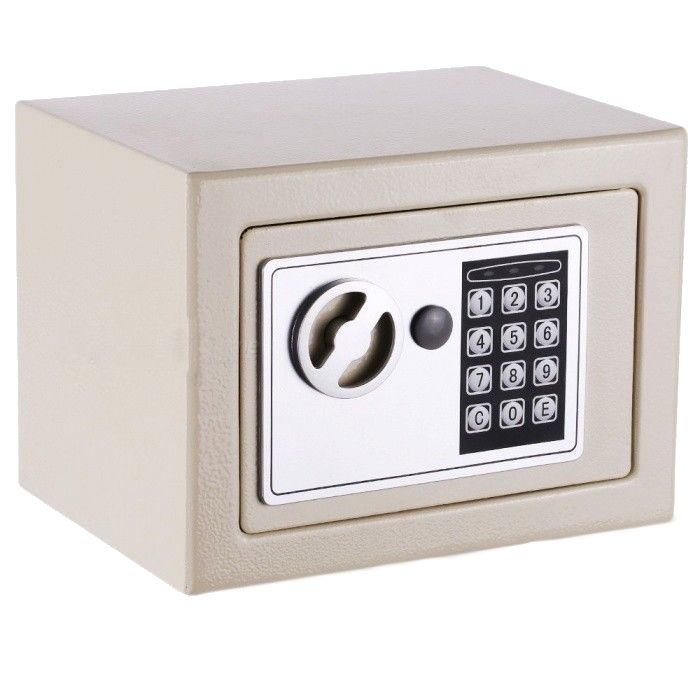
\includegraphics[height = .8\textheight]{safe_guard}
    \caption{Example of target for side-channel attack}
  \end{figure}

  \note{

    Идея атак по сторонним каналам \textbf{весьма стара}, ещё в 1980-х годах
    было о них известно. Но широкое распространение данный вид атак получил
    только после публикации \textbf{Пола Кохера в 1996 году}.

    Самый примитивный пример атаки по сторонним каналам --- \textbf{определение
      нажатых кнопок сейфа по звуку} при введении секретного кода.

    Такого рода атаки обычно основываются на вычислении изменений в окружающей
    среде, например, изменения в \textbf{потреблении тока устройством,
      электромагнитном излучении, температуре, по издаваемым акустическим
      сигналам, по времени,} затрачиваемому на выполнение тех или иных операций
    и другие.

  }
\end{frame}

\subsection{Microarchitectural attacks}
\begin{frame}[fragile]{\insertsubsection}


  \begin{columns}
    \begin{column}{.3\textwidth}
      \begin{minted}[]{nasm}
        code1a:
          mov (X), %eax
          mov (Y), %ebx
          clflush (X)
          clflush (Y)
          jmp code1a
      \end{minted}
    \end{column}

    \begin{tikzpicture}
      \draw[line width = 3pt, -{Stealth[length = 1cm]}] (0,0) -- (3,0);
    \end{tikzpicture}

    \begin{column}{.5\textwidth}
      \begin{figure}[h]
        \center%
        
\includegraphics[width = .6\textwidth]{cpu_break}
        \caption{The DRAM cells get permanently damaged if hammered for a long
          time}
      \end{figure}
    \end{column}
  \end{columns}

  \note{

    Атаки по сторонним каналам на микроархитектуру, основанные на использовании
    программного обеспечения, как правило, даже \textbf{не требуют физического
      доступа} к вычислительному устройству.

    Также существуют атаки, \textbf{основанные на дефектах микроархитектуры},
    например, ошибки, происходящие \textbf{во время оптимизации}.

    Атаки на микроархитектуру, которые используют аппаратные дефекты,
    \textbf{сложно воссоздать на практике,}. Примеров таких атак не много, но
    все они широко известны, это например, \textbf{Rowhammer атака,} которая, в
    случае успешно разработанного потока инструкций, может дестабилизировать
    работу процессора и даже нанести \textbf{неисправимые физические
      повреждения,} если атака будет проводиться в течении нескольких недель.

    \textbf{Все уязвимости можно найти, просто почитав} главу оптимизаций в
    \textbf{спецификации процессора}, даже на Wiki есть раздел про оптимизацию
    работы CPU, в которой перечислены все элементы, в которых были найдены
    уязвимости.

  }

\end{frame}


% ------------------------------------------------------------------------------

\section{Theory}
\subsection{CPU}
\begin{frame}{\insertsubsection}

  \begin{figure}[h]
    \center%
    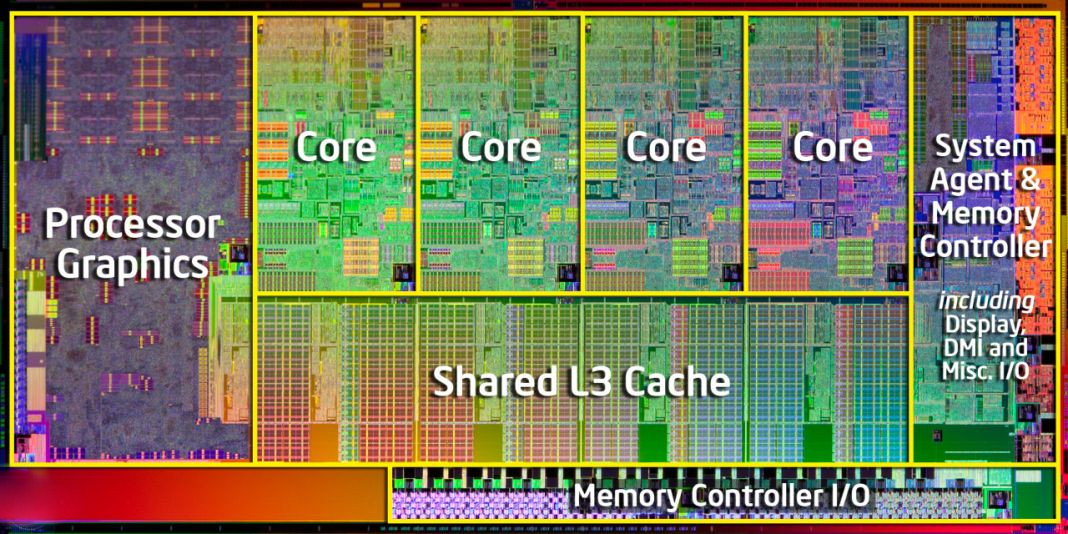
\includegraphics[height = .7\textheight]{multicore_cpu}
    \caption{Architecture of multicore CPU}
  \end{figure}

  \note{

    Современные процессоры состоят из множества крупных элементов:
    \textbf{ядер}, \textbf{графического процессора}, \textbf{общего кэша},
    \textbf{контроллера памяти} и других.

  }
\end{frame}

\begin{frame}<1-2>[label = core_elements]{\insertsubsection}

  \begin{columns}
    \column{.2\textwidth}%
      Abstract architecture of core and memory organization
    \column{.8\textwidth}%
    \begin{figure}[h]
      \center%
      \begin{tikzpicture}[
        align = center,
        ->,
        > = Stealth,
        mmu_node/.style = {
          rectangle,
          draw = dGreen,
        },
        cpu_node/.style = {
          rectangle,
          draw = dViolet,
        },
        mem_node/.style = {
          rectangle,
          draw = dBlue,
        },
        ]

        \node[mmu_node] (cr3) {CR3};

        \node[below = .5 of cr3,
        mmu_node,
        ] (pt_walker) {PT Walker};

        \node[left = of pt_walker,
        mmu_node,
        ] (tlb) {TLB};

        \node[
        inner sep = 8,
        fit = (tlb) (pt_walker) (cr3),
        draw = dGray,
        label = above left:\color{dBlue}MMU,
        ] (mmu) {};

        \node[
        cpu_node,
        left = 2cm of mmu,
        yshift = 20,
        ] (exec_unit)  {Execution Unit};

        \node[
        cpu_node,
        below = .8 of exec_unit,
        ] (load_unit) {Load/Store Unit};

        \node[mem_node,
        below = .6 of mmu,
        ] (l1_data) {L1 Data};

        \node[
        inner sep = 15,
        fit = (mmu) (load_unit) (exec_unit) (l1_data),
        draw = dGray,
        label = 151:\color{dBlue}Core,
        ] (core) {};

        \node[mem_node, below = .2 of core] (l3) {%
          L3 (Shared)};

        \node[mem_node, above = .75 of l3] (l2) {%
          L2};

        \node<2>[
        fit = (exec_unit) (load_unit),
        line width = 0.5mm,
        draw = dRed,
        ] (fit_exec) {};

        \node<3>[
        fit = (l1_data) (l2) (l3),
        line width = 0.5mm,
        draw = dRed,
        ] (fit_cache) {};

        \node<4>[
        fit = (tlb) (pt_walker) (cr3),
        line width = 0.5mm,
        draw = dRed,
        ] (fit_mmu) {};

        \path (cr3)                edge                                       (pt_walker)
              (mmu)                edge node[right] {Phys. addr.}             (l1_data)
              (l1_data)            edge                                       (l2)
              (l2)                 edge[<->]                                  (l3);

        \draw (pt_walker.165) -> node[above = 0cm] {Fill} (pt_walker.165 -| tlb.east);
        \draw (tlb.330) -> node[above = 0cm] {Miss} (tlb.330 -| pt_walker.west);
        \draw[<->] (exec_unit.east) -- node[below = .3cm] {Virt. addr.} (exec_unit -| mmu.west);
        \draw[<->] (load_unit.east) -- (load_unit -| mmu.west);

      \end{tikzpicture}
      % \caption{Abstract architecture of core and memory
      %   organization}\label{fig:core_elements}
    \end{figure}
  \end{columns}

  \note<1>{

    На рисунке \ref{fig:core_elements} представлен общий \textbf{план работы
      ядра с памятью и кэшем} в Intel процессорах. Более подробно об алгоритмах
    работы будет рассказано ниже.

    Современные процессоры представляют из себя \textbf{сильно
      распараллеливанные машины}, которые оперируют данными на высоких
    скоростях. Размеры процессоров уменьшаются, уменьшается потребление памяти
    используемое для вычисления одной и той же операции, что позволяет
    \textbf{увеличивать тактовую частоту}. Однако, существуют и другие способы
    уменьшить время, затрачиваемое на выполнение инструкций ---
    \textbf{различные оптимизации}, типы которых зависят от данных и состояния
    процессора.

    Рассмотрим некоторые \textbf{системы оптимизации, применяемые в ядрах и
      процессоре}.

  }

  \note<2->{

    Ниже \textbf{будет рассказано} о работе этих элементов.

  }
\end{frame}

\subsubsection{Pipelining}
\begin{frame}{\insertsubsubsection. In-Order}

  \begin{columns}
    \column{.3\textwidth}%
      Elements of a modern in-order core
    \column{.7\textwidth}
    \begin{figure}[h]
      \begin{tikzpicture}[
        draw,
        align = center,
        ->,
        > = Stealth,
        node distance = .5,
        block/.style = {
          rectangle,
          draw = dGreen,
          text centered,
        },
        ]

        \node[block] (l1_i) {L1 I\$};

        \node[block, below = of l1_i] (if) {Instruction Fetch};

        \node[block, below = of if] (id) {Instruction Decode};

        \node[block, below = of id] (ie) {Instruction Execute};

        \node[block, below = of ie] (mem_acc) {Memory Access};

        \node[block, below = of mem_acc] (write) {Writeback};

        \node[block, left = of if] (bp) {Branch Predictor};

        \node[block, left = of mem_acc] (rf) {Register File};

        \node[block, right = 1.5 of mem_acc] (l1_d) {L1 D\$};

        \path (l1_i)    edge      (if)
              (if)      edge      (id)
              (id)      edge      (ie)
              (ie)      edge      (mem_acc)
              (mem_acc) edge      (write)
              (if)      edge      (bp)
              (l1_d)    edge[<->] (mem_acc);

        \draw (rf.north)   |- node{} (ie.west);
        \draw (write.west) -| node{} (rf.south);
        \draw (bp.south)   |- node{} (id.west);

      \end{tikzpicture}
      % \caption{Elements of a modern in-order core}\label{fig:exe_in_order}
    \end{figure}
  \end{columns}

  \note{

    Конвейеризация --- одна из главных причин высокой скорости работы
    процессора. В результате данного процесса \textbf{работа с инструкциями
      разделяется} на несколько этапов (рисунок \ref{fig:exe_in_order},
    \textbf{выполнение инструкций по порядку}):

    \begin{itemize}
    \item \textbf{этап получения}, в результате которого код операции инструкции
      загружается в процессор;

    \item \textbf{этап декодирования}, в результате которого опкод декодируется
      во внутреннее представление процессора;

    \item \textbf{этап выполнения} --- инструкция исполняется.
    \end{itemize}

  }
\end{frame}

% \begin{frame}{\insertsubsubsection. Не по порядку}
%   \begin{figure}[h]
%     \center%
%     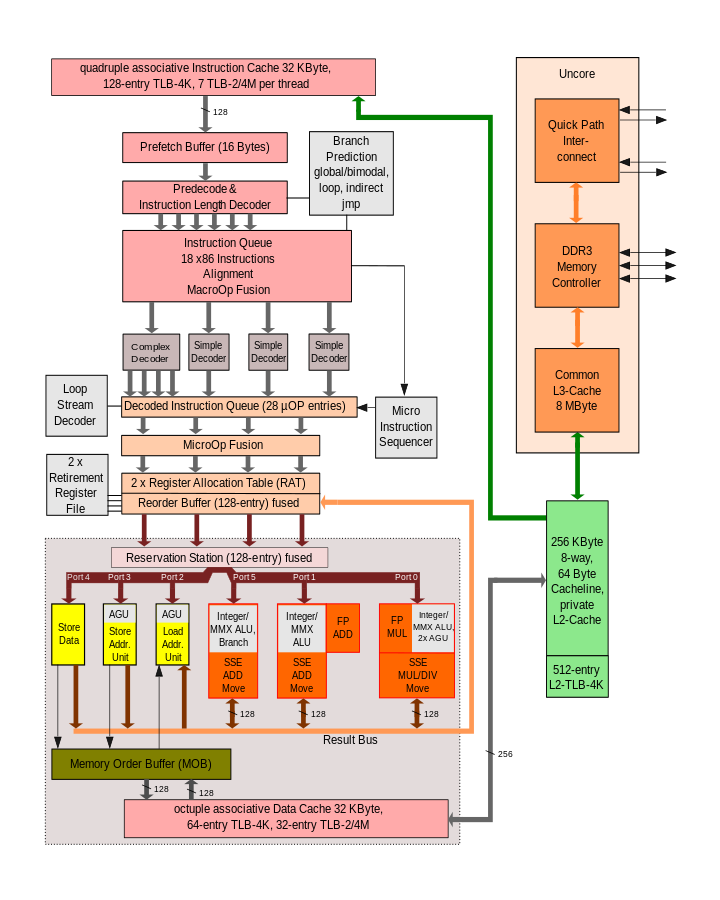
\includegraphics[height = .8\textheight]{Intel_Nehalem_arch}
%     \caption{Микроархитектура Intel Nehalem в 4-х ядерной реализации}
%   \end{figure}

%   \note{

%     На слайде представлено более полное описание микроархитектуры, но мы же
%     \textbf{рассмотрим упрощённую версию}.

%   }
% \end{frame}

\begin{frame}<1>[label = reorder_exe]{\insertsubsubsection. Out-of-Order}

  \begin{columns}
    \column{.2\textwidth}
      Elements of a modern out-of-order core
    \column{.8\textwidth}
    \begin{figure}[h]
      \begin{tikzpicture}[
        align = center,
        ->,
        > = Stealth,
        node distance = .5,
        block/.style = {
          rectangle,
          draw = dGreen,
        },
        ]

        \node[block] (l1_i) {L1 I\$};

        \node[block, below = .3 of l1_i,
        rectangle split,
        rectangle split parts = 2] (if_id) {%
          Instruction Fetch%
          \nodepart{two}%
          Instruction Decode%
        };

        \node[block, left = 1 of if_id] (bp) {Branch Predictor};

        \node[block, below = of if_id] (rob) {Register Renaming (ROB)};

        \node[block, below left = of rob.south] (iprf) {Integer Physical %
          Register File};

        \node[block, below right = of rob.south] (vprf) {Vector Physical %
          Register File};

        \node[block, below = 1.2cm of rob] (eu) {Execution Units};

        \node[block, below = of eu] (l1_d) {L1 D\$};

        \node[block,
        minimum height = 4cm,
        minimum width = .5cm,
        right = 3cm of rob] (l2) {L2};

        \node<2>[
        fit = (bp),
        inner sep = 0pt,
        line width = 0.5mm,
        draw = dRed,
        ] (fit_bp) {};

        \node<2>[
        fit = (rob),
        inner sep = 0pt,
        line width = 0.5mm,
        draw = dRed,
        ] (fit_rob) {};

        \path (l1_i)  edge      (if_id)
              (if_id) edge[<->] (bp)
              (eu)    edge[<->] (l1_d);

        \draw (rob) -| (iprf.north);
        \draw (rob) -| (vprf.north);
        \draw (iprf) |- (eu.west);
        \draw (vprf) |- (eu.east);

        \foreach \i [count = \xi from 0] in {2,...,-2}{
          \draw ([xshift = \i * 0.4cm]if_id.south) -- ([xshift = \i * 0.4cm]rob.north);
        }

        \draw[<->] (l1_i) -| (l2.north);
        \draw[<->] (l1_d) -| (l2.south);

      \end{tikzpicture}
      % \caption{Elements of a modern out-of-order core}\label{fig:exe_out_of_order}
    \end{figure}
\end{columns}

  \note<1>{

    Рисунок \ref{fig:exe_out_of_order}, \textbf{выполнение инструкций не по
      порядку}.

    Инструкции получаются и декодируются по порядку во \textbf{front-end}.

    \textbf{ROB} --- \textbf{Re-Order Buffer}.

    Именно поэтому процессор может выполнять несколько инструкций
    \textbf{одновременно}, при этом не обязательно в порядке их следования.
    Современные процессоры также могут параллельно выполнять одни и те же стадии
    для оптимизации вычислений.

  }

  \note<2->{

    О работе Reorder Buffer \textbf{рассказано не будет}, существует множество
    его реализаций.

    Ниже \textbf{будет рассказано} о работе этих элементов.

  }
\end{frame}

% \begin{frame}{\insertsubsubsection. Не по порядку}

%   \begin{figure}[h]
%     \begin{tikzpicture}[
%       align = center,
%       ->,
%       > = Stealth,
%       thick,
%       double = ForestGreen,
%       double distance = 1pt,
%       % node distance = .6,
%       c_node/.style = {
%         circle,
%         draw,
%         fill = ForestGreen,
%         text = White,
%         minimum width = 1cm,
%         text width = .5cm,
%         text centered,
%       },
%       block/.style = {
%         rectangle,
%         draw,
%         fill = ForestGreen,
%         text = White,
%         minimum width = 3cm,
%         text width = 3cm,
%         text centered,
%       },
%       ]

%       \node[block,
%       rectangle split,
%       rectangle split parts = 6] (code) {
%         R1 = LOAD A \\
%         \nodepart{two}
%         R2 = LOAD B \\
%         \nodepart{three}
%         R3 = R1 + R2 \\
%         \nodepart{four}
%         R1 = 1 \\
%         \nodepart{five}
%         R2 = 2 \\
%         \nodepart{six}
%         R3 = R1 + R2 \\
%       };

%       \node[c_node, right = 3 of code.north east] (r1_1) {
%         R1
%       };

%       \node[c_node, right = of r1_1] (r2_1) {
%         R2
%       };

%       \node[c_node, below = of $(r1_1)!0.5!(r2_1)$,
%       label = right:Есть зависимость от данных] (r3_1) {
%         R3
%       };

%       \node[c_node, below = 2 of r1_1] (r1_2) {
%         R1
%       };

%       \node[c_node, right = of r1_2] (r2_2) {
%         R2
%       };

%       \node[c_node, below = of $(r1_2)!0.5!(r2_2)$,
%       label = right:Нет зависимости от данных] (r3_2) {
%         R3
%       };

%       \path (r1_1) edge (r3_1)
%       (r2_1) edge (r3_1)
%       (r1_2) edge (r3_2)
%       (r2_2) edge (r3_2);

%     \end{tikzpicture}
%     \caption{Пример выполнения инструкций не по
%       порядку}\label{fig:exe_out_of_order_example}
%   \end{figure}

%   \note{

%     Представлен пример кода, который имеет и зависимые, и независимые от других
%     данных участки. \textbf{На следующем слайде} будет представлено, как RoB
%     обрабатывает такой код.

%   }
% \end{frame}

% \begin{frame}{\insertsubsubsection. Не по порядку}

%   \begin{columns}
%     \begin{column}{.3\textwidth}
%       \begin{figure}[h]
%         \center
%         \begin{tikzpicture}[
%           align = center,
%           thick,
%           block/.style = {
%             rectangle,
%             draw,
%             text = White,
%             minimum width = 3cm,
%             text width = 3cm,
%             text centered,
%           },
%           ]

%           \node[block,
%           rectangle split,
%           rectangle split parts = 6,
%           rectangle split part fill = {Maroon, Maroon, Maroon, ForestGreen, ForestGreen, ForestGreen},
%           ] (code) {
%             R1 = LOAD A \\
%             \nodepart{two}
%             R2 = LOAD B \\
%             \nodepart{three}
%             R3 = R1 + R2 \\
%             \nodepart{four}
%             R1 = 1 \\
%             \nodepart{five}
%             R1 = 2 \\
%             \nodepart{six}
%             R3 = R1 + R2 \\
%           };
%         \end{tikzpicture}
%         \caption{Порядок выполнения}
%       \end{figure}
%     \end{column}

%     \begin{tikzpicture}
%       \draw[line width = 3pt, -{Stealth[length = 1cm]}] (-2,0) -- (0,0);
%     \end{tikzpicture}

%     \begin{column}{.6\textwidth}
%       \begin{table}[h]
%         \begin{tabular}{|c|m{1.4cm}|c|m{1.3cm}|m{1cm}|}
%           \hline
%           №&Имя регистра&Инструкция&Зависи\-мости&Гото\-во?\\
%           \hline%
%           \rowcolor{Maroon}%
%           \color{White}1&\color{White}P1 = R1&\color{White}P1 = LOAD A&\color{White}-&\color{White}-\\
%           \hline%
%           \rowcolor{Maroon}%
%           \color{White}2&\color{White}P2 = R2&\color{White}P2 = LOAD B&\color{White}-&\color{White}-\\
%           \hline%
%           \rowcolor{Maroon}%
%           \color{White}3&\color{White}P3 = R3&\color{White} P3 = P1 + P2&\color{White} 1, 2&\color{White}-\\
%           \hline%
%           \rowcolor{ForestGreen}%
%           \color{White}4&\color{White}P4 = R1&\color{White}P4 = 1&\color{White}-&\color{White}+\\
%           \hline%
%           \rowcolor{ForestGreen}%
%           \color{White}5&\color{White}P5 = R2&\color{White}P5 = 1&\color{White}-&\color{White}+\\
%           \hline%
%           \rowcolor{ForestGreen}%
%           \color{White}6&\color{White}P6 = R3&\color{White}P6 = P4 + P5&\color{White}4, 5&\color{White}-\\
%           \hline%
%         \end{tabular}
%         \caption{Re-Order Buffer (ROB)}
%       \end{table}
%     \end{column}
%   \end{columns}

%   \note{

%     RoB \textbf{внутри себя производит трансляцию} в требуемый ему вид,
%     переименовывает регистры, реорганизует опкоды.

%     Именно по этой причине код может исполняться внутри процессора не по
%     порядку.

%   }

% \end{frame}

\againframe<2>{reorder_exe}

\subsubsection{Branch Prediction and Speculation}
\begin{frame}{\insertsubsubsection}


  \begin{figure}[h]
    \begin{tikzpicture}[
      align = center,
      ->,
      > = Stealth,
      block/.style = {
        rectangle,
        draw = dGreen,
        minimum width = 4cm,
        text width = 4cm,
        text centered,
      },
      ]

      \node[block] (if) {\texttt{if x > y}};

      \node[block, below left = of if.center] (secret) {%
        \texttt{get\_secret\_key()}%
      };

      \node[block, below right = of if.center] (comp) {%
        \texttt{some\_computation()}%
      };

      \draw (if.west) -| node[above] {$\omega = 0.80$} (secret.north);
      \draw (if.east) -| node[above] {$\omega = 0.53$} (comp.north);

    \end{tikzpicture}
    \caption{\texttt{get\_secret\_key()} can be executed
      speculatively}\label{fig:if_speculative_example}
  \end{figure}

  \note{

    Ещё одна идея для повышения производительности процессора ---
    \textbf{исполнение инструкций спекулятивно}. С помощью такой оптимизации
    процессор \textbf{угадывает возможный переход и исполняет его} прежде, чем
    он может выполниться на самом деле. Если угаданный путь был верным, то
    процессор просто берёт информацию, которую получил заранее, в противном
    случае \textbf{информация} о ходе спекулятивного выполнения просто
    \textbf{удаляется}.

    Существуют:

    \begin{itemize}
    \item Статическое предсказание
    \item Динамическое предсказание
      \begin{itemize}
      \item счётчик с насыщением
      \item адаптивный двухуровневый предсказатель
      \item локальный предсказатель перехода
      \item глобальный предсказатель перехода
      \item гибридный предсказатель перехода
      \item предсказатель для цикла
      \item предсказатель косвенных переходов
      \item предсказатель инструкций возврата
      \item предсказатель, основанный на машинном обучении
      \end{itemize}
    \end{itemize}

  }
\end{frame}

\subsubsection{Multicore}
\begin{frame}{\insertsubsubsection}

  \begin{figure}[h]
    \center%
    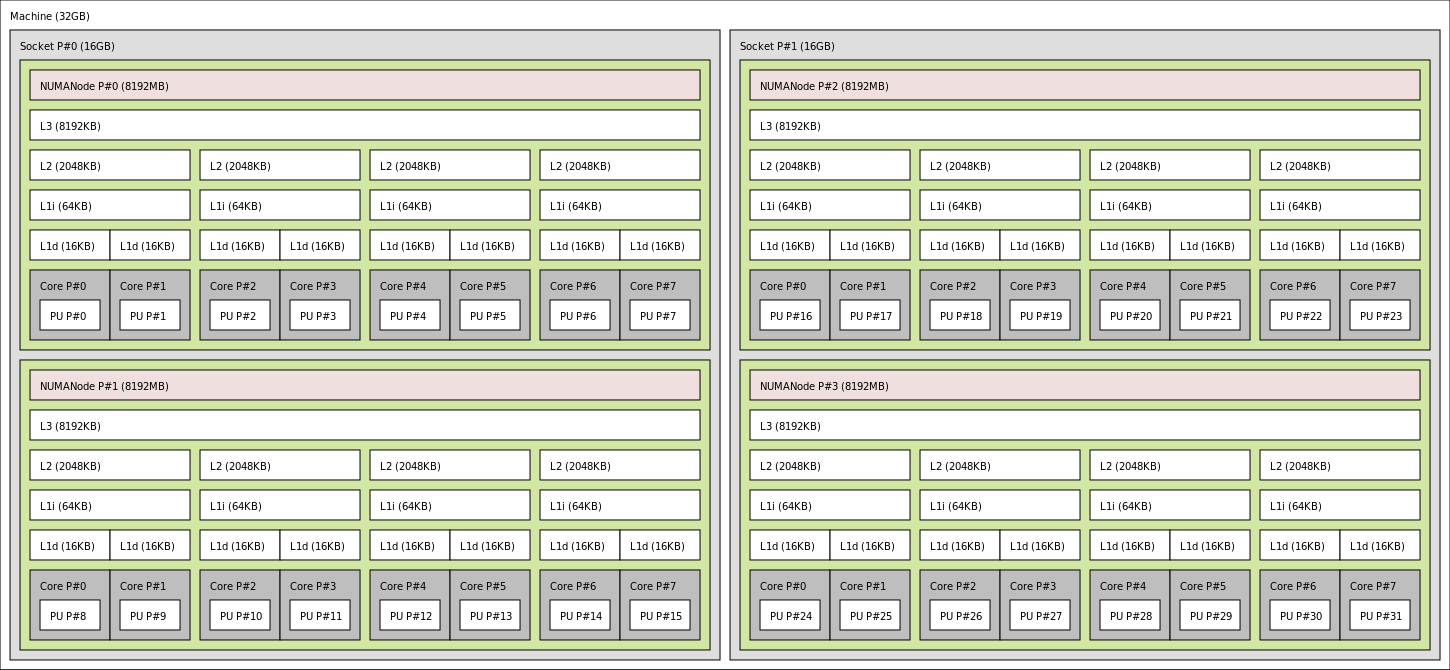
\includegraphics[height = .7\textheight]{Hwloc}
    \caption{Architecture of multicore CPU AMD Bulldozer}
  \end{figure}

  \note{

    Вместо оптимизации скорости выполнения на единственном ядре, также
    существует возможность \textbf{увеличивать количество этих самых ядер}.
    Особенно часто много ядер установлено в процессорах, работающих на серверах,
    это позволяет выполнять многие независимые друг от друга задачи параллельно.
    Однако, если задачу невозможно распараллелить, то прироста в
    производительности, конечно же, не будет. В настоящее время, \textbf{почти
      любое устройство имеет несколько ядер}, в том числе IoT устройства и
    домашние компьютеры. К тому же, многие языки программирования позволяют без
    лишних сложностей писать приложения, которые будут исполнятся на нескольких
    ядрах. \textbf{Каждое} из таких \textbf{ядер имеет свои приватные ресурсы},
    например, регистры и конвейеры выполнения, а также \textbf{общие ресурсы},
    например, основной доступ к памяти.

  }
\end{frame}


\subsection{Cache}
\againframe<3>{core_elements}

\begin{frame}{\insertsubsection}

  \begin{figure}
    \begin{tikzpicture}[
      align = center,
      ->,
      > = Stealth,
      core/.style = {
        rectangle,
        inner sep = 5pt,
        draw = dBlue,
      },
      cache1/.style = {
        rectangle split,
        rectangle split horizontal,
        rectangle split parts = 2,
        draw = dGreen,
      },
      cache2/.style = {
        rectangle,
        draw = dViolet,
      },
      cache3/.style = {
        rectangle,
        draw = dDarkGray,
      },
      block/.style = {
        rectangle,
        draw = dRed,
      },
      ]

      \node[
      core,
      ] (core_0) {Core 0};

      \node[
      core,
      right = 2.2cm of core_0,
      ] (core_1) {Core 1};

      \node[
      core,
      right = 2.2cm of core_1,
      ] (core_2) {Core 2};

      \node[
      core,
      right = 2.2cm of core_2,
      ] (core_3) {Core 3};

      \node[
      cache1,
      below = .7 of core_0.center,
      ] (c1_0) {%
        32KB, L1-i%
        \nodepart{two}%
        32KB, L1-d%
      };

      \node[
      cache1,
      below = .7 of core_1.center,
      ] (c1_1) {%
        32KB, L1-i%
        \nodepart{two}%
        32KB, L1-d%
      };

      \node[
      cache1,
      below = .7 of core_2.center,
      ] (c1_2) {%
        32KB, L1-i%
        \nodepart{two}%
        32KB, L1-d%
      };

      \node[
      cache1,
      below = .7 of core_3.center,
      ] (c1_3) {%
        32KB, L1-i%
        \nodepart{two}%
        32KB, L1-d%
      };

      \node[
      cache2,
      below = .5 of c1_0,
      ] (c2_0) {256KB,\\L2 (NINE)};

      \node[
      cache2,
      below = .5 of c1_1,
      ] (c2_1) {256KB,\\L2 (NINE)};

      \node[
      cache2,
      below = .5 of c1_2,
      ] (c2_2) {256KB,\\L2 (NINE)};

      \node[
      cache2,
      below = .5 of c1_3,
      ] (c2_3) {256KB,\\L2 (NINE)};

      \node[
      cache3,
      below = .5 of $(c2_1.south)!.5!(c2_2.south)$,
      ] (c3) {8MB, shared L3 (inclusive L1, L2)};

      % TODO
      % Dirty hack
      \node[
      below = .80 of c3,
      ] (caption_hack) {Data flow through a modern platform};

      \node[
      block,
      minimum width = 2cm,
      right = 2.5 of c3,
      ] (mc) {MC};

      \node[
      block,
      minimum width = 2cm,
      left = 2.5 of c3,
      ] (ht) {HT};

      \node[
      block,
      minimum width = 2cm,
      below = .5 of mc,
      ] (dram) {DRAM};

      \node[
      block,
      minimum width = 2cm,
      below = .5 of ht,
      ] (chips) {Other chips};

      \draw[<->] (core_0) -- (c1_0);
      \draw[<->] (core_1) -- (c1_1);
      \draw[<->] (core_2) -- (c1_2);
      \draw[<->] (core_3) -- (c1_3);

      \draw[<->] (c1_0) -- (c2_0);
      \draw[<->] (c1_1) -- (c2_1);
      \draw[<->] (c1_2) -- (c2_2);
      \draw[<->] (c1_3) -- (c2_3);
      \draw[<->] (c2_0) -- ++(1.5, 0) -- ++(0, -1) |- (c3.175);
      \draw[<->] (c2_1.south) -- (c2_1.south |- c3.north);
      \draw[<->] (c2_2.south) -- (c2_2.south |- c3.north);
      \draw[<->] (c2_3) -- ++(-1.5, 0) -- ++(0, -1) |- (c3.5);

      \draw[<->] (c3) -- (ht);
      \draw[<->] (c3) -- (mc);

      \draw[<->] (ht) -- (chips);
      \draw[<->] (mc) -- (dram);

    \end{tikzpicture}
    % \caption{Data flow through a modern platform}\label{fig:proc_cache_arch}
  \end{figure}

  \note{

    Современные процессоры имеют целую \textbf{иерархию кэшей} с различными
    размерами и скоростью обращения. Некоторые кэши приватные и работают в
    контексте \textbf{только одного процессора}, \textbf{некоторые общие}, их
    могут читать и писать все процессоры.

    Существует несколько \textbf{правил включения (инклюзивности) кэша} один в
    другой: правило \textbf{инклюзивности}, \textbf{эксклюзивности},
    \textbf{NINE}.

    HT --- HyperTransport; MC --- Memory Controller.

  }

\end{frame}

\begin{frame}{\insertsubsection}

  \begin{figure}[h]

    \newcommand*\virtcolor{dGreen, dGreen, dGreen, dGreen, dGreen, dGreen}

    \only<2-3>{

      \renewcommand*\virtcolor{dGreen, dGreen, dRed, dGreen, dGreen, dGreen}

    }

    \begin{tikzpicture}[
      align = center,
      ->,
      > = Stealth,
      block/.style = {
        draw = dWhite,
        text = dWhite,
        minimum width = 2cm,
        rectangle split,
        rectangle split parts = 6,
        rectangle split part fill = {
          dGreen, dGreen, dGreen, dGreen, dGreen, dGreen
        },
      },
      cache/.style = {
        draw = dWhite,
        text = dWhite,
        text centered,
        minimum width = 2cm,
        rectangle split,
        rectangle split parts = 2,
        rectangle split part fill = {
          dGray, dGray
        },
      },
      ]

      \node[block,
      rectangle split part fill = {\virtcolor},
      label = above:Virtual memory,
      ] (virt) {%
        0xf200%
        \nodepart{two}%
        0xf100%
        \nodepart{three}%
        0xf000%
        \nodepart{four}%
        $\cdots$%
        \nodepart{five}%
        0x3000%
        \nodepart{six}%
        0x2000%
      };

      \node[cache,
      right = of virt,
      label = above:Address,
      ] (cache_addr) {
        \only<1-3>{0xf200}%
        \only<4>{0xf000}%
        \nodepart{two}%
        0x2000%
      };

      \node[cache,
      right = 0 of cache_addr,
      label = above:Data,
      fill = dBlue,
      text = dWhite,
      ] (cache_content) {
        \only<1-3>{Kernel secret 0}%
        \only<4>{Kernel secret 1}%
        \nodepart{two}%
        User secret%
      };

      \node[rectangle,
      fit = (cache_addr) (cache_content),
      label = {below:Cache (L1, L2, LLC)},
      inner sep = 0,
      ] {};

      \node[block,
      right = of cache_content,
      label = above:Physical memory (DRAM),
      ] (phys) {%
        0x1000%
        \nodepart{two}%
        0x0900%
        \nodepart{three}%
        0x0800%
        \nodepart{four}%
        0x0700%
        \nodepart{five}%
        0x0600%
        \nodepart{six}%
        0x0500%
      };

      \draw<1>[dGreen] (virt.one east)  -- ++(.5, 0) -- node[right] {hit} ++(0, -1) |- (cache_addr.one west);
      \draw<1>[dGreen] (virt.five east) -- ++(.5, 0) -- node[below right] {hit} ++(0, .4) |- (cache_addr.two west);

      \draw<1-3> (phys.three west) -- (cache_content.one east);
      \draw (phys.four west) -- (cache_content.two east);

      \draw<2>[dRed] (virt.east) -- node[above] {miss} (cache_addr.west);

      \draw<3>[dRed] (virt.three east) -- ++(.5, 0) -- ++(0, -3) -| (phys.south);

      \draw<4> (virt.three east) -- ++(.5, 0) -- ++(0, -3) -| (phys.south);
      \draw<4>[dRed] (phys.six west) -- ++(-.3, 0) |- (cache_content.one east);

    \end{tikzpicture}
    \caption{CPU cache algorithm}\label{fig:cache_manipulation_example}
  \end{figure}

  \note<1>{

    В общем случае, все доступы к памяти происходят через кеш. Если доступ к
    памяти происходит через кеш, то это называется \textbf{попаданием кэша}
    (\textit{cache hit}).

  }

  \note<2> {

    В противном случае происходит \textbf{промах кэша} (\textit{cache miss}).

  }

  \note<3> {

    Данные берутся из медленной памяти.

  }

  \note<4> {

    В кэш записываются новые данные.

  }

\end{frame}

\subsubsection{Types of cache}
\begin{frame}{\insertsubsubsection}
  \begin{itemize}
  \item Direct-mapped cache
  \item Fully-associative cache
  \item 2/4/8/12-way set associative cache
  \end{itemize}

  \note{

    \begin{enumerate}
    \item Главная \textbf{проблема} такого вида кэша --- это то, что кэш может
      \textbf{хранить единственную} линию кэша из всех \textbf{конгруэнтных}.
      Следовательно, если процессору требуется работать с двумя или более
      конгруэнтными линиями кэша, то такого рода кэш будет совершать
      \textbf{множество промахов}.
    \item Такие кэши становятся более \textbf{дорогими с увеличением путей}.
      Поэтому они обычно содержат небольшое количество путей, например, в
      современных процессорах используются \textbf{буферы ассоциативной
        трансляции (translation-lookaside buffers TLB)} с 64 путями.
    \end{enumerate}
    
  }
\end{frame}

% \subsubsection{Кэш с прямым отображением}
% \begin{frame}{\insertsubsubsection}


%   \begin{figure}[h]
%     \begin{tikzpicture}[
%       align = center,
%       ->,
%       > = Stealth,
%       thick,
%       ampersand replacement = \&,
%       mem/.style = {
%         draw,
%         minimum width = 2cm,
%         rectangle split,
%         rectangle split parts = 3,
%         rectangle split horizontal,
%         rectangle split every empty part = {},
%         rectangle split empty part width = width("n бит"),
%       },
%       cache/.style = {
%         matrix of nodes,
%         nodes in empty cells,
%         nodes = {
%           minimum width = 3cm,
%           minimum height = .8cm,
%           draw,
%           align = center,
%           anchor = center,
%         },
%         right delimiter = \},
%       },
%       ]

%       \node[cache,
%       label = above:Кэш,
%       label = {
%         [label distance = 10]right:$2^n$\\линий\\кэша
%       },
%       ] (cache) {
%         Тег \& Данные \\
%         \& \\
%         \& \\
%         \& \\
%       };

%       \node[
%       below = of cache-3-2,
%       ] (b_bits) {
%         Смещение в данных на $2^b$ байт
%       };

%       \node[mem,
%       left = of cache-1-1.west,
%       label = above:Адрес памяти,
%       ] (addr) {
%         \nodepart{two}
%         \textit{n} бит
%         \nodepart{three}
%         \textit{b} бит
%         \nodepart{four}
%       };

%       \node[
%       draw,
%       dashed,
%       below = of addr.one south,
%       rectangle,
%       minimum width = 1cm,
%       minimum height = 1cm,
%       ] (f) {
%         f
%       };

%       \node[
%       circle,
%       draw,
%       below = of cache-4-1,
%       ] (hit) {
%         hit?
%       };

%       \node[below = .5 of hit] (final) {};

%       \draw (addr.one south) -> (f);
%       \draw (f) |- node[below right] {Тег} (hit);
%       \draw (hit) -> (final);
%       \draw (cache-3-1.center) -> (hit);
%       \draw (addr.two south) |- node[below right] {Индекс кэша} (cache-3-1.west);
%       \draw (b_bits) -> (cache-3-2.center);


%     \end{tikzpicture}
%     % \caption{Схема работы кэша с прямым
%     %   отображением}\label{fig:directly_mapped_cache}
%   \end{figure}

%   \note{

%     Кэш состоит из $2^n$ \textbf{линий кэша}, каждая линия содержит \textbf{тег}
%     и $2^b$ байт \textbf{ассоциированных данных}. Тег вычисляется из
%     соответствующего адреса памяти, который добавляется в эту кэш линию.
%     \textbf{Тег используется} в дальнейшем для того, чтобы определять
%     \textbf{присутствие} того или иного адреса в линии кэша. Последние
%     \textit{b} бит адреса \textbf{используются} в качестве \textbf{смещения для
%       данных} в линии кэша. Современные процессоры имеют длину линии кэша в
%     \textit{64 байта}, т. е. \texttt{b = 6}. \textbf{Средние} \textit{n} бит
%     адреса памяти \textbf{используются в качестве \textit{индекса кэша}},
%     который говорит о номере линии кэша, в котором содержатся данные.

%     Размер кэша определяет, как много бит будет использовано, т. е. как много
%     индексов будет использовано. \textbf{Адреса с теми же \textit{n} битами}
%     являются \textbf{конгруэнтными}, так как они отображают те же линии кэша.

%     Главная \textbf{проблема} такого вида кэша --- это то, что кэш может
%     \textbf{хранить единственную} линию кэша из всех конгруэнтных.
%     Следовательно, если процессору требуется работать с двумя или более
%     конгруэнтными линиями кэша, то такого рода кэш будет совершать множество
%     промахов.

%   }

% \end{frame}

% \subsubsection{Полностью ассоциативный кэш}
% \begin{frame}{\insertsubsubsection}

%   \newcommand*\nodeonecolor{White}
%   \newcommand*\nodetwocolor{White}
%   \newcommand*\nodethreecolor{White}
%   \newcommand*\arrowonecolor{Black}
%   \newcommand*\arrowtwocolor{Black}
%   \newcommand*\arrowthreecolor{Black}

%   \only<2>{
%     \renewcommand*\nodeonecolor{Red}
%     \renewcommand*\arrowonecolor{Red}
%   }
%   \only<3>{
%     \renewcommand*\nodetwocolor{Red}
%     \renewcommand*\arrowtwocolor{Red}
%   }
%   \only<4>{
%     \renewcommand*\nodethreecolor{ForestGreen}
%     \renewcommand*\arrowthreecolor{ForestGreen}
%   }

%   \begin{figure}[h]
%     \begin{tikzpicture}[
%       align = center,
%       ->,
%       > = Stealth,
%       thick,
%       ampersand replacement = \&,
%       mem/.style = {
%         draw,
%         minimum width = 2cm,
%         rectangle split,
%         rectangle split parts = 2,
%         rectangle split horizontal,
%         rectangle split every empty part = {},
%         rectangle split empty part width = width("bbbbbbbbbbbbbbb"),
%       },
%       cache/.style = {
%         matrix of nodes,
%         nodes in empty cells,
%         nodes = {
%           minimum width = 3cm,
%           minimum height = .8cm,
%           draw,
%           align = center,
%           anchor = center,
%         },
%       },
%       ]

%       \node[cache,
%       label = above:Кэш,
%       ] (cache) {
%         Тег \& Данные \\
%         \& \\
%         \& \\
%         \& \\
%       };

%       \node[mem,
%       left = of cache-1-1.west,
%       label = above:Адрес памяти,
%       ] (addr) {
%         \nodepart{two}
%         \textit{b} бит
%         \nodepart{three}
%       };

%       \node[
%       draw,
%       dashed,
%       below = of addr.one south,
%       rectangle,
%       minimum width = 1cm,
%       minimum height = 1cm,
%       ] (f) {
%         f
%       };

%       \node[
%       fill = \nodeonecolor,
%       text = Black,
%       circle,
%       draw,
%       below = 2cm of cache-2-1,
%       ] (hit_1) {
%         \only<1>{hit?}
%         \only<2->{miss}
%       };

%       \node[
%       fill = \nodetwocolor,
%       text = Black,
%       circle,
%       draw,
%       below right = 0.1 of hit_1,
%       ] (hit_2) {
%         \only<1-2>{hit?}
%         \only<3->{miss}
%       };

%       \node[
%       fill = \nodethreecolor,
%       text = Black,
%       circle,
%       draw,
%       below right = 0.1 of hit_2,
%       ] (hit_3) {
%         \only<1-3>{hit?}
%         \only<4->{hit!}
%       };

%       \node<4>[below = of cache-4-2] (data) {
%         Данные
%       };

%       \draw (addr.one south) -> (f);
%       \draw (f) |- node[below right] {Тег} (hit_1);
%       \draw (f) |- (hit_2);
%       \draw (f) |- (hit_3);
%       \draw[\arrowonecolor] (cache-2-1.center) -> (hit_1);
%       \draw[\arrowtwocolor] ([xshift = 0.8cm]cache-3-1.center) -> (hit_2);
%       \draw[\arrowthreecolor] ([xshift = 1cm]cache-4-1.center) -> (hit_3);
%       \draw<4>[\arrowthreecolor] (cache-4-2.center) -> (data);


%     \end{tikzpicture}
%     % \caption{Схема работы полностью ассоциативного
%     %   кэша}\label{fig:fully_associative_cache}
%   \end{figure}

%   \note<1>{

%     Проблема конгруэнтности \textbf{решается в полностью ассоциативном кэше}.

%     Такой вид кэша не содержит индексов и каких-либо линий кэша. Вместо этого он
%     хранит множество \textbf{путей кэша}, которые в свою очередь содержат
%     данные. \textbf{Тег} теперь \textbf{используется для определения
%       существования адреса в кэше} и какой именно путь кэша содержит
%     ассоциированные данные.

%     \textbf{Пример на следующих слайдах!}

%   }

%   \note<2->{

%     Такие кэши становятся более \textbf{дорогими с увеличением путей}. Поэтому
%     они обычно содержат небольшое количество путей, например, в современных
%     процессорах используются \textbf{буферы ассоциативной трансляции
%       (translation-lookaside buffers TLB)} с 64 путями.

%   }

% \end{frame}

\subsubsection{Two-way set associative cache}
\begin{frame}{\insertsubsubsection}

  \begin{figure}[h]
    \begin{tikzpicture}[
      align = center,
      ->,
      > = Stealth,
      ampersand replacement = \&,
      mem/.style = {
        draw,
        minimum width = 2cm,
        rectangle split,
        rectangle split parts = 3,
        rectangle split horizontal,
        rectangle split every empty part = {},
        rectangle split empty part width = width("n bits"),
      },
      cache/.style = {
        matrix of nodes,
        nodes in empty cells,
        nodes = {
          font = \scriptsize,
          minimum width = 3cm,
          minimum height = .6cm,
          draw,
          align = center,
          anchor = center,
        },
        right delimiter = \},
      },
      ]

      \node[cache,
      label = above:Cache,
      label = {%
        [label distance = 10]right:$2^n$\\sets%
      },
      ] (cache) {%
        \node[fill = dGray!20](cache_1_1){Way 1 Tag}; \& \node[fill = dGray!20]{Way 1 Data};\\
        \node{Way 2 Tag}; \& \node{Way 2 Data};\\
        \node[fill = dGray!20](tag_1){}; \& \node[fill = dGray!20](data_1){};\\
        \node(tag_2){}; \& \node(data_2){};\\
        \node[fill = dGray!20]{}; \& \node[fill = dGray!20]{};\\
        % \node{}; \& \node{}; \\
        % \node[fill = dGray!20]{}; \& \node[fill = dGray!20]{}; \\
      };

      \node[mem,
      left = of cache_1_1.west,
      label = above:Memory Address,
      ] (addr) {%
        \nodepart{two}%
        \textit{n} bits%
        \nodepart{three}%
        \textit{b} bits%
      };

      \node[
      rectangle,
      draw,
      dashed,
      below = of addr.one south,
      minimum width = 1cm,
      minimum height = 1cm,
      ] (f) {f};

      \node[
      circle,
      draw,
      below = of tag_2,
      ] (hit_1) {hit?};

      \node[
      circle,
      draw,
      below right = 0.1 of hit_1,
      ] (hit_2) {hit?};

      \draw (addr.one south) -> (f);
      \draw (f) |- node[below right] {Tag} (hit_1);
      \draw (f) |- node[below right] {}    (hit_2);
      \draw (addr.two south) |- node[below right] {Cache index} (cache.west);

      \draw (tag_1.center) -> (hit_1);
      \draw ([xshift = 0.8cm]tag_2.center) -> (hit_2);

    \end{tikzpicture}
    % \caption{How works two-way associative
    %   cache}\label{fig:set_associative_cache}
  \end{figure}

  \note{

    Компромиссом между этими двумя видами кэша оказывается \textbf{кеш с
      наборами}, а не с линиями кэша. Данные кэши широко используются в
    современных процессорах, где их называют \textbf{\textit{m}-путейные (или
      \textit{m}-входовые) кэши с ассоциативным набором}. Рисунок отображает
    абстрактную модель 2-путейного кэша данного вида.

    Кэш делится на $2^n$ набора. \textbf{Индекс набора} в кэше определяется
    средними \textbf{n} битами адреса. Каждый набор имеет \textbf{m путей} для
    возможности хранения местоположения \textbf{m конгруэнтных адресов}. Наборы
    кэша могут быть также представлены в виде крошечного полностью
    ассоциативного кэша с \textit{m} путями для набора конгруэнтных адресов.
    Поэтому \textbf{тег} снова используется для определения какой путь кэша
    \textbf{содержит определённый адрес}.

  }

\end{frame}

\subsubsection{Cache replacement policies}
\begin{frame}{\insertsubsubsection}

  \begin{columns}

    \column{.5\textwidth}
    \begin{itemize}
      \item \texttt{FIFO}
      \item \texttt{LIFO}
      \item least recently used, \texttt{LRU}
      \item time aware least recently used, \texttt{TLRU}
      \item most recently used, \texttt{MRU}
      \item pseudo-LRU, \texttt{PLRU}
      \item random replacement, \texttt{RR}
      \item segment LRU, \texttt{SLRU}
    \end{itemize}
    \column{.5\textwidth}
    \begin{itemize}
      \item least frequently used, \texttt{LFU}
      \item least frequent recently used, \texttt{LFRU}
      \item LFU with dynamic aging, \texttt{LFUDA}
      \item low inter--reference recency set, \texttt{LIRS}
      \item adaptive replacement cache, \texttt{ARC}
      \item clock with adaptive replacement, \texttt{CAR}
      \item multi queue, \texttt{MQ}
      \item and etc.
    \end{itemize}
  \end{columns}

  \note{

    \textbf{Количество путей или линий в кэше ограничено}, а
    \textbf{конгруэнтных адресов}, которые требуется хранить, ---
    \textbf{достаточно много}, требуется производить замены данных в кэше на
    новые, полученные из главной памяти.

    Производители процессоров хранят детали этих правил в \textbf{секрете}, так
    как данные правила очень сильно влияют на скорость работы процессора в
    целом.

    Самое широкое распространение получили правила вытеснения
    \textbf{«вытеснение давно неиспользуемых» (least-recently used, LRU)}.

    Процессоры \textbf{ARM} обычно используют правила \textbf{случайного
      вымещения}, так как такие правила просто реализовать на аппаратных
    средствах, и в ходе своей работы они потребляют мало энергии, а также
    показывают себя высокопроизводительными.

  }

\end{frame}

\subsubsection{Addressing modes}
\begin{frame}{\insertsubsubsection}
  \begin{itemize}
  \item Virtually indexed, virtually tagged (VIVT)
  \item Physically indexed, virtually tagged (PIVT)
  \item Virtually indexed, physically tagged (VIPT)
  \item Physically indexed, physically tagged (PIPT)
  \end{itemize}

  \note{

    Кэши могут использовать как \textbf{виртуальные адреса}, так и
    \textbf{физические для вычисления индекса кэша и тега}. На практике
    используется три способа вычисления данных.

    Позволяет использовать \textbf{тег из физического адреса}, при этом
    небольшая задержка, так как для поиска в первую очередь и чаще всего
    требуется определить номер набора, который задан виртуальным адресом.

    \begin{itemize}
    \item уникальный тег --- \textbf{возможность применять разделяемые данные}
    \item всё происходит быстро, потому что \textbf{трансляция} адреса
      происходит \textbf{параллельно} поиску \textbf{индекса кэша}
    \end{itemize}

  }
\end{frame}

% \subsubsection{Режимы адресации}
% \begin{frame}{\insertsubsubsection. VIVT}

%   \begin{figure}[h]
%     \begin{tikzpicture}[
%       align = center,
%       ->,
%       > = Stealth,
%       thick,
%       ampersand replacement = \&,
%       mem/.style = {
%         draw,
%         minimum width = 2cm,
%         rectangle split,
%         rectangle split parts = 3,
%         rectangle split horizontal,
%         rectangle split every empty part = {},
%         rectangle split empty part width = width("n бит"),
%       },
%       cache/.style = {
%         matrix of nodes,
%         nodes in empty cells,
%         nodes = {
%           font = \scriptsize,
%           minimum width = 3cm,
%           minimum height = .6cm,
%           draw,
%           align = center,
%           anchor = center,
%         },
%         right delimiter = \},
%         text = Black,
%       },
%       ]

%       \node[cache,
%       label = above:Кэш,
%       label = {
%         [label distance = 10]right:$2^n$\\наборов\\кэша
%       },
%       ] (cache) {
%         \node[fill = black!30]{Тег 1-го пути}; \& \node[fill = black!30]{Данные 1-го пути}; \\
%         \node[fill = black!10]{Тег 2-го пути}; \& \node[fill = black!10]{Данные 2-го пути}; \\
%         \node[fill = black!30](tag_1){}; \& \node[fill = black!30](data_1){}; \\
%         \node[fill = black!10](tag_2){}; \& \node[fill = black!10](data_2){}; \\
%         \node[fill = black!30]{}; \& \node[fill = black!30]{}; \\
%         \node[fill = black!10]{}; \& \node[fill = black!10]{}; \\
%         \node[fill = black!30]{}; \& \node[fill = black!30]{}; \\
%       };

%       \node[mem,
%       left = of cache-1-1.west,
%       label = above:Виртуальный адрес памяти,
%       ] (addr) {
%         \nodepart{two}
%         \textit{n} бит
%         \nodepart{three}
%         \textit{b} бит
%         \nodepart{four}
%       };

%       \node[
%       draw,
%       dashed,
%       below = of addr.one south,
%       rectangle,
%       minimum width = 1cm,
%       minimum height = 1cm,
%       ] (f) {
%         f
%       };

%       \node[
%       circle,
%       draw,
%       below = of cache-4-1,
%       ] (hit_1) {
%         hit?
%       };

%       \draw (addr.one south) -> (f);
%       \draw (addr.two south) |- node[below right] {Индекс\\ набора кэша} (cache.west);

%       \draw (f) |- node[below right] {Тег} (hit_1);

%       \draw (tag_1.center) -> (hit_1);

%     \end{tikzpicture}
%     \caption{Виртуальная индексация виртуальное
%       тагетирование}\label{fig:vivt_cache}
%   \end{figure}

%   \note{

%     Кэши могут использовать как \textbf{виртуальные адреса}, так и
%     \textbf{физические для вычисления индекса кэша и тега}. На практике
%     используется три способа вычисления данных.

%     \begin{itemize}
%     \item Виртуальный тег не уникален при переключении контекста ---
%       \textbf{данные не могут быть разделяемыми}
%     \item Трансляция адреса не происходит --- \textbf{быстрая скорость работы}
%     \end{itemize}

%     \textbf{Виртуальная индексация виртуальное тагетирование (virtually-indexed
%       virtually-tagged VIVT)}. Используется для маленьких данных, с которыми
%     производятся быстрые операции, в \textbf{ARM процессорах} используются в
%     качестве \textbf{кэша инструкций}.

%   }
% \end{frame}

% \begin{frame}{\insertsubsubsection. PIPT}

%   \begin{figure}[h]
%     \begin{tikzpicture}[
%       align = center,
%       ->,
%       > = Stealth,
%       thick,
%       ampersand replacement = \&,
%       mem/.style = {
%         draw,
%         minimum width = 2cm,
%         rectangle split,
%         rectangle split parts = 3,
%         rectangle split horizontal,
%         rectangle split every empty part = {},
%         rectangle split empty part width = width("n бит"),
%       },
%       cache/.style = {
%         matrix of nodes,
%         nodes in empty cells,
%         nodes = {
%           font = \scriptsize,
%           minimum width = 3cm,
%           minimum height = .6cm,
%           draw,
%           align = center,
%           anchor = center,
%         },
%         right delimiter = \},
%         text = Black,
%       },
%       ]

%       \node[cache,
%       label = above:Кэш,
%       label = {
%         [label distance = 10]right:$2^n$\\наборов\\кэша
%       },
%       ] (cache) {
%         \node[fill = black!30]{Тег 1-го пути}; \& \node[fill = black!30]{Данные 1-го пути}; \\
%         \node[fill = black!10]{Тег 2-го пути}; \& \node[fill = black!10]{Данные 2-го пути}; \\
%         \node[fill = black!30](tag_1){}; \& \node[fill = black!30](data_1){}; \\
%         \node[fill = black!10](tag_2){}; \& \node[fill = black!10](data_2){}; \\
%         \node[fill = black!30]{}; \& \node[fill = black!30]{}; \\
%         \node[fill = black!10]{}; \& \node[fill = black!10]{}; \\
%         \node[fill = black!30](point){}; \& \node[fill = black!30]{}; \\
%       };

%       \node[mem,
%       left = of cache-1-1.west,
%       label = above:Виртуальный адрес памяти,
%       ] (addr) {
%         \nodepart{two}
%         \textit{n} бит
%         \nodepart{three}
%         \textit{b} бит
%         \nodepart{four}
%       };

%       \node[
%       draw,
%       dashed,
%       below = .5 of addr,
%       xshift = -.6cm,
%       ] (tlb) {
%         TLB
%       };

%       \node[mem,
%       below = 1.6 of addr,
%       ] (addr_phys) {
%         \nodepart{two}
%         \textit{n} бит
%         \nodepart{three}
%         \textit{b} бит
%         \nodepart{four}
%       };

%       \node[
%       draw,
%       dashed,
%       below = .5 of addr_phys.one south,
%       rectangle,
%       minimum width = 1cm,
%       minimum height = 1cm,
%       ] (f) {
%         f
%       };

%       \node[
%       circle,
%       draw,
%       below = of cache-4-1,
%       ] (hit_1) {
%         hit?
%       };

%       \draw (addr_phys.one south) -> (f);
%       \draw (addr_phys.two south) |- node[below right] {Индекс\\ набора кэша} (point);

%       \draw (addr.205) -> (tlb);
%       \draw (tlb) -> (addr_phys.155);
%       \draw (addr.three south) -> (addr_phys.three north);

%       \draw (f) |- node[below right] {Тег} (hit_1);

%       \draw (tag_1.center) -> (hit_1);

%     \end{tikzpicture}
%     \caption{Физическая индексация физическое
%       тагетирование}\label{fig:pipt_cache}
%   \end{figure}

%   \note{

%     \textbf{Физическая индексация физическое тагетирование (physically-indexed
%       physically-tagged PIPT)}. Используется \textbf{тег и индекс из физического
%       адреса}.

%     \begin{itemize}
%     \item Тег будет уникальным даже при смене контекста --- \textbf{разделяемая
%         память будет реально разделяемой}
%     \item Смена контекста --- \textbf{большие задержки}
%     \end{itemize}

%     Используется для кэшей данных и инструкций, задержка по большей части
%     уменьшается посредством использования кэшей в системе трансляции адресов
%     (TLB).

%   }

% \end{frame}

% \begin{frame}{\insertsubsubsection. VIPT}

%   \begin{figure}[h]
%     \begin{tikzpicture}[
%       align = center,
%       ->,
%       > = Stealth,
%       thick,
%       ampersand replacement = \&,
%       mem/.style = {
%         draw,
%         minimum width = 2cm,
%         rectangle split,
%         rectangle split parts = 3,
%         rectangle split horizontal,
%         rectangle split every empty part = {},
%         rectangle split empty part width = width("n бит"),
%       },
%       cache/.style = {
%         matrix of nodes,
%         nodes in empty cells,
%         nodes = {
%           font = \scriptsize,
%           minimum width = 3cm,
%           minimum height = .6cm,
%           draw,
%           align = center,
%           anchor = center,
%         },
%         right delimiter = \},
%         text = Black,
%       },
%       ]

%       \node[cache,
%       label = above:Кэш,
%       label = {
%         [label distance = 10]right:$2^n$\\наборов\\кэша
%       },
%       ] (cache) {
%         \node[fill = black!30]{Тег 1-го пути}; \& \node[fill = black!30]{Данные 1-го пути}; \\
%         \node[fill = black!10]{Тег 2-го пути}; \& \node[fill = black!10]{Данные 2-го пути}; \\
%         \node[fill = black!30](tag_1){}; \& \node[fill = black!30](data_1){}; \\
%         \node[fill = black!10](tag_2){}; \& \node[fill = black!10](data_2){}; \\
%         \node[fill = black!30]{}; \& \node[fill = black!30]{}; \\
%         \node[fill = black!10]{}; \& \node[fill = black!10]{}; \\
%         \node[fill = black!30]{}; \& \node[fill = black!30]{}; \\
%       };

%       \node[mem,
%       left = of cache-1-1.west,
%       label = above:Виртуальный адрес памяти,
%       ] (addr) {
%         \nodepart{two}
%         \textit{n} бит
%         \nodepart{three}
%         \textit{b} бит
%         \nodepart{four}
%       };

%       \node[
%       draw,
%       dashed,
%       below = .5 of addr,
%       xshift = -.6cm,
%       ] (tlb) {
%         TLB
%       };

%       \node[mem,
%       below = 1.6 of addr,
%       ] (addr_phys) {
%         \nodepart{two}
%         \textit{n} бит
%         \nodepart{three}
%         \textit{b} бит
%         \nodepart{four}
%       };

%       \node[
%       draw,
%       dashed,
%       below = .5 of addr_phys.one south,
%       rectangle,
%       minimum width = 1cm,
%       minimum height = 1cm,
%       ] (f) {
%         f
%       };

%       \node[
%       circle,
%       draw,
%       below = of cache-4-1,
%       ] (hit_1) {
%         hit?
%       };

%       \draw (addr_phys.one south) -> (f);
%       \draw (addr.two south) |- node[below right] {Индекс\\ набора кэша} (tag_1);

%       \draw (addr.205) -> (tlb);
%       \draw (tlb) -> (addr_phys.155);
%       \draw (addr.three east) -- ++(0.7, 0) -- ++(0, -1) |- (addr_phys.three east);

%       \draw (f) |- node[below right] {Тег} (hit_1);

%       \draw (tag_1.center) -> (hit_1);

%     \end{tikzpicture}
%     \caption{Виртуальная индексация физическое
%       тагетирование}\label{fig:vipt_cache}
%   \end{figure}

%   \note{

%     \textbf{Виртуальная индексация физическое тагетирование (virtually-indexed
%       physically-tagged VIPT).}

%     Позволяет использовать \textbf{тег из физического адреса}, при этом
%     небольшая задержка, так как для поиска в первую очередь и чаще всего
%     требуется определить номер набора, который задан виртуальным адресом.

%     \begin{itemize}
%     \item уникальный тег --- \textbf{возможность применять разделяемые данные}
%     \item всё происходит быстро, потому что \textbf{трансляция} адреса
%       происходит \textbf{параллельно} поиску \textbf{индекса кэша}
%     \end{itemize}

%   }

% \end{frame}


\subsection{DRAM}
\subsubsection{How DRAM works}
\begin{frame}{\insertsubsubsection}

  \newcommand*\dramcolor{dWhite, dWhite, dWhite, dWhite, dWhite, dWhite, dWhite}

  \only<2>{
    \renewcommand*\dramcolor{dWhite, dWhite, dGreen, dWhite, dWhite, dWhite,
      dWhite}
  }

  \begin{figure}[h]
    \begin{tikzpicture}[
      align = center,
      ->,
      > = Stealth,
      barstyle/.style 2 args = {%
        draw = dBlue,
        minimum width = 2em,
        fit = {(####1.south) (####1.north)},
        inner ysep = 0pt,
        label = {[rotate = 90]center:####2}
      },
      ]

      \node[
      draw = dGreen,
      minimum width = 2cm,
      ] (proc) {CPU};


      \node[
      draw = dGreen,
      right = 3 of proc,
      ] (mmu) {Memory controller};

      \node[
      draw = dGreen,
      right = 3 of mmu,
      rectangle split,
      rectangle split parts = 7,
      rectangle split part fill = {\dramcolor},
      minimum width = 2cm,
      ] (dram) {%
        Row 0%
        \nodepart{two}%
        Row 1%
        \nodepart{three}%
        Row 2%
        \nodepart{four}%
        Row 3%
        \nodepart{five}%
        Row 4%
        \nodepart{six}%
        Row 5%
        \nodepart{seven}%
        Row 6%
        \nodepart{seven}%
        Row 7%
      };

      \node[
      barstyle={dram}{%
        \only<1>{Row buffer}%
        \only<2>{Row 2}%
      },
      left = 0 of dram,
      ] (r_buf) {};


      \node[
      fit = (dram) (r_buf),
      label = above:DRAM array,
      ] {};

      \draw (proc) -- node[above] {Memory bus} (mmu);
      \draw (mmu) -- node[above] {Request} (r_buf);

    \end{tikzpicture}
    \caption{A simple computer system with a single DRAM
      array}\label{dram_example}
  \end{figure}

  \note<1>{

    \textbf{DRAM (dynamic random-access memory, динамическая память с
      произвольным доступом).}

    DRAM имеет большую задержку в сравнении с кэш-памятью. Причина большой
    задержки не только в том, что ячейки DRAM имеют меньшую тактовую частоту, но
    и в том, как DRAM организован и подключён к процессору. Современные
    процессоры используют чипы-контроллеры памяти, которые позволяют
    передавать/получать данные в/с DRAM.


    DRAM содержит: \textbf{строки (row)} и \textbf{колонки (columns)} (обычно
    1024).

  }

  \note<2>{

    Строка может быть \textbf{открытой} и \textbf{закрытой}. Если какая-либо
    строка открыта, то она вся сохраняется в \textbf{буфер строки (row buffer)}.

    Если текущая открытая строка содержит необходимые данные, то контроллер
    памяти просто берёт их из буфера строки. Эта ситуация очень похожа на кэш
    попадание и называется \textbf{попадание строки}. Если текущая открытая
    строка не содержит нужных данных, то это называется \textbf{промах строки}.
    \textbf{Контроллер памяти} в таком случае сначала \textbf{закрывает строку},
    т. е. \textbf{записывает буфер строки обратно в DRAM}, а затем
    \textbf{открывает нужную строку} и считывает данные из буфера строки. Также
    как и промахи кэша, промахи строки вызывают повышение задержки.

  }

\end{frame}

\subsubsection{DRAM organization}
\begin{frame}{\insertsubsubsection}

  \begin{figure}[h]
    \begin{tikzpicture}[
      align = center,
      ->,
      > = Stealth,
      bank/.style = {
        draw = dGreen,
        rectangle split,
        rectangle split parts = 3,
      },
      ]

      \node<1>[inner sep = 0, label = above:DIMM] (dram) {%
        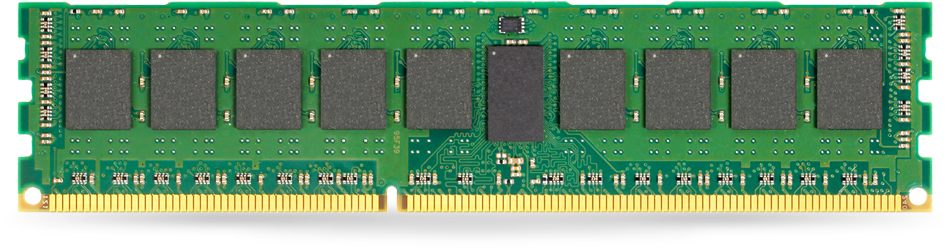
\includegraphics[height = .3\textheight]{DRAM_ddr4}%
      };

      \node<2-4>[inner sep = 0] (dram_0) {%
        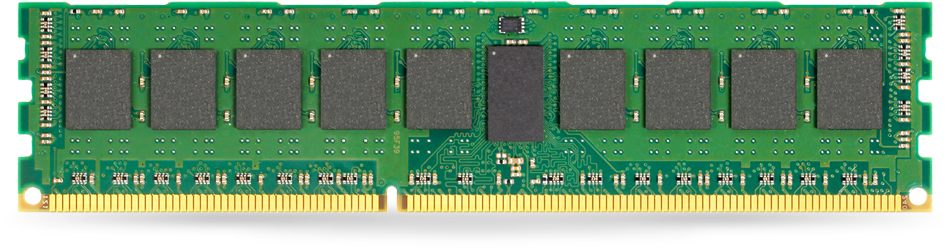
\includegraphics[height = .2\textheight]{DRAM_ddr4}%
      };

      \node<2-4>[inner sep = 0, below = of dram_0] (dram_1) {%
        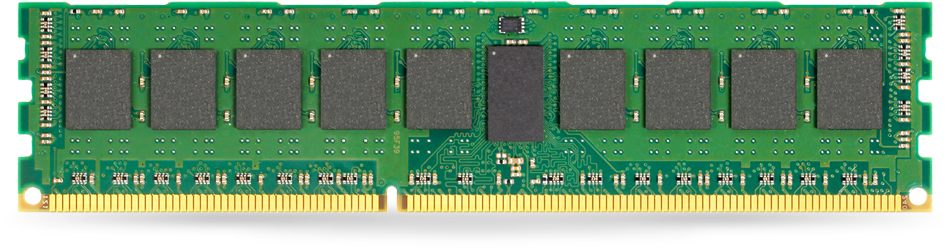
\includegraphics[height = .2\textheight]{DRAM_ddr4}%
      };

      \node<2-4>[
      inner sep = 0,
      left = 2cm of $(dram_0.west)!.5!(dram_1.west)$,
      ] (cpu) {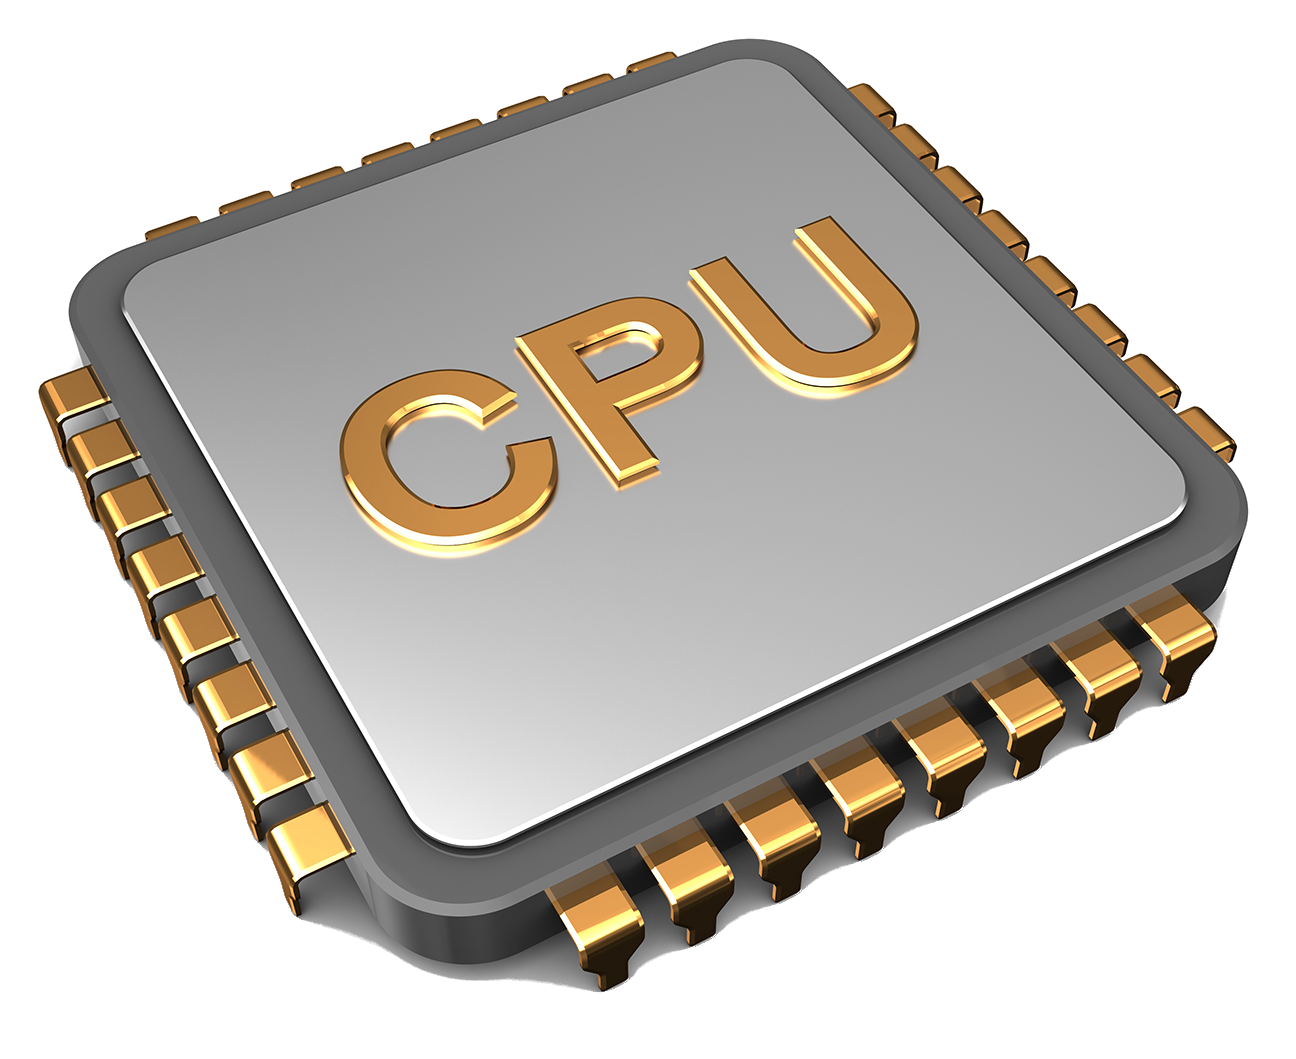
\includegraphics[height = .3\textheight]{cpu}};

      \draw<2-4> (cpu) -- ++(2, 0) -- ++(0, 1)  |- node[above] {Channel 0} (dram_0.west);
      \draw<2-4> (cpu) -- ++(2, 0) -- ++(0, -1) |- node[below] {Channel 1} (dram_1.west);

      \node<3-4>[
      right = 0.3 of dram_0,
      ] (rank_0) {Front of DIMM:\\rank 0};

      \draw<3-4> (dram_0) to [out = 80, in = 60, looseness = 8]%
          node[above] {Back of DIMM: rank 1} (dram_0);
      \draw<3-4> (dram_0) -> (rank_0);

      \draw<4>[dRed,
      rounded corners,
      very thick,
      ] (2.10, -2.7) rectangle (2.67, -2.0);

      \node<4> (chip_capt) at (3.5, -2.4) {Chip};

      \node<5>[bank,
      ] (bank_0) {%
        Row 0%
        \nodepart{two}%
        $\cdots$%
        \nodepart{three}%
        Row 32767%
      };

      \node<5>[
      rectangle,
      draw = dBlue,
      below = .1 of bank_0,
      ] (r_buf_0) {Row buffer};

      \node<5>[
      fit = (bank_0) (r_buf_0),
      draw,
      label = above:Bank 0,
      ] {};

      \node<5>[bank,
      right = of bank_0,
      ] (bank_1) {%
        Row 0%
        \nodepart{two}%
        $\cdots$%
        \nodepart{three}%
        Row 32767%
      };

      \node<5>[
      rectangle,
      draw = dBlue,
      below = .1 of bank_1,
      ] (r_buf_1) {Row buffer};

      \node<5>[
      fit = (bank_1) (r_buf_1),
      draw,
      label = above:Bank 1,
      ] {};

      \node<5>[bank,
      right = of bank_1,
      ] (bank_n) {%
        Row 0%
        \nodepart{two}%
        $\cdots$%
        \nodepart{three}%
        Row 32767%
      };

      \node<5>[
      rectangle,
      draw = dBlue,
      below = .1 of bank_n,
      ] (r_buf_n) {Row buffer};

      \node<5>[
      fit = (bank_n) (r_buf_n),
      draw,
      label = above:Bank n,
      ] {};

      \node<5>[
      rectangle,
      draw = dGreen,
      minimum width = 2cm,
      minimum height = 2cm,
      above = of bank_1,
      label = above:Chip,
      ] (chip) {%
        Bank 0\\%
        Bank 1\\%
        $\cdots$\\%
        Bank n%
      };

      \node<6>[
      rectangle split,
      rectangle split parts = 5,
      rectangle split horizontal,
      draw = dGreen,
      label = above:Row of DRAM,
      ] (dram_row) {%
        Cell 0%
        \nodepart{two}%
        Cell 1%
        \nodepart{three}%
        Cell 2%
        \nodepart{four}%
        $\cdots$%
        \nodepart{five}%
        Cell n%
      };

      \node<6>[
      below = of dram_row,
      ] (cap) {Capacitor};

      \draw<6> (cap) -> (dram_row.one south);
      \draw<6> (cap) -> (dram_row.two south);
      \draw<6> (cap) -> (dram_row.three south);
      \draw<6> (cap) -> (dram_row.five south);

    \end{tikzpicture}
    % \caption{DRAM organization}\label{dram_arch}
  \end{figure}

  \note<1>{

    Для повышения производительности работы с DRAM были использованы те же
    методы, что и в случае с кэшем. Современные компьютерные системы
    организовывают DRAM в виде \textbf{каналов}, \textbf{DIMM (Dual Inline
      Memory Modules)}, \textbf{рангов} и \textbf{банков}.

    Количество памяти увеличивается в разы при перемножении количества банков на
    количество \textbf{DIMM модулей}.

  }

  \note<2>{

    Для \textbf{увеличения ширины потока данных} и увеличения количества
    параллельных потоков современные компьютерные системы используют
    \textbf{несколько каналов}. Каждый канал управляется независимо и
    параллельно через DRAM шину.

  }

  \note<3>{

    Современные модели DRAM имеют обычно от \textbf{1 до 4 рангов}, количество
    которых увеличивается при перемножении с количеством банков. Такого рода
    параллелизм позволяет \textbf{уменьшить промах строки}.

  }

  \note<5>{

    Каждый из этих банков имеет своё собственное состояние и может иметь
    \textbf{независимо от других банков} открытую строку.

    Современная DDR3 DRAM память имеет 8 банков, а DDR4 DRAM 16 банков (на
    ранг).

  }

  \note<6> {

    В случае если два адреса \textbf{отображаются на пространство одного и того
      же} DIMM модуля, ранга и банка, то эти адреса физически
    \textbf{расположены рядом друг с другом} в DRAM. В таких случаях два адреса
    оказываются в банке с одним и тем же номером. В случае, если адреса
    отображаются на пространство банков с одним и тем же номером, но разных
    рангов или DIMM'ов, то они не расположены физически рядом.

    Также как и с кэшем, существуют функции, которые производят отображение
    физического адреса на конкретные канал, DIMM, ранг и банк. Как работают эти
    функции, публично известно только у AMD, Intel не публиковала никакой
    информации. Однако, относительно недавно (2015, 2016) был произведён
    реверс-инжиниринг данных функций. Знание того, \textbf{как производится
      отображение физического адреса на физические структуры} даёт нам новый
    вектор атак --- \textbf{атаки по сторонним каналам на DRAM}.

  }

\end{frame}

%%% \subsection{Виртуальная память}
%%% \subsubsection{Изолирование памяти}
\begin{frame}{\insertsubsubsection}

  \begin{figure}[h]
    \begin{tikzpicture}[
      align = center,
      ->,
      > = Stealth,
      thick,
      block/.style = {
        rectangle,
        draw,
        text = White,
        minimum width = 14cm,
        text width = 14cm,
        minimum height = 1.5cm,
        text centered,
      },
      ]

      \node[block, fill = ForestGreen] (user) {
        Пользовательское пространство
      };

      \node[block, below = 2 of user, fill = Maroon] (kernel) {
        Пространство операционной системы (ядра ОС)
      };

      \draw[double, <->] (user) -- node[right] {Интерфейс системных вызовов} (kernel);

    \end{tikzpicture}
    \caption{Система изолирования памяти}\label{fig:userspace_kernel_space}
  \end{figure}

  \note{

    Так как мультипроцессорная обработка данных становится всё популярнее, то и
    \textbf{задача изолирования памяти различных процессов} также становится
    актуальнее.

    Существует программная изоляция в виде разделения на
    \textbf{пользовательское пространство} и \textbf{пространство} операционной
    системы (\textbf{ядра ОС}).

  }
\end{frame}

\begin{frame}{\insertsubsubsection}

  \begin{figure}[h]
    \begin{tikzpicture}[
      align = center,
      ->,
      > = Stealth,
      thick,
      block/.style = {
        rectangle,
        draw,
        text = White,
        text centered,
      },
      ]

      \node (cat) {
        \texttt{\$ cat /proc/self/maps}
      };

      \node[block,
      font = \ttfamily,
      rectangle split,
      rectangle split parts = 9,
      rectangle split part fill = {
        Maroon, Maroon, Maroon,
        ForestGreen, ForestGreen, ForestGreen,
        PineGreen, ForestGreen, ForestGreen},
      below = of cat,
      ] (virt) {
        0xffff\_ffff\_1234\_0000
        \nodepart{two}
        $\cdots$
        \nodepart{three}
        0xffff\_ffff\_1200\_00c0
        \nodepart{four}
        $\cdots$
        \nodepart{five}
        0x7f90\_00c9\_8000
        \nodepart{six}
        $\cdots$
        \nodepart{seven}
        0x7ffc\_8f5b\_8000
        \nodepart{eight}
        $\cdots$
        \nodepart{nine}
        0x5637\_6a5f\_3000
      };

      \node[right = of virt.seven east] (vdso) {
        VDSO \\
        (Virtual Dynamic Shared Object)
      };

      \draw[->] (vdso) -- (virt.seven east);

    \end{tikzpicture}
    \caption{Пример карты памяти для процесса
      \texttt{cat}}\label{fig:cat_memory_map}
  \end{figure}

  \note{

    Также на первых порах была введена такая технология, как \textbf{виртуальная
      память}, которая представляла из себя \textbf{изолированные сегменты,
      ссылающиеся на физическую память}. На уровне виртуальной памяти
    операционная система могла иметь определённые права доступа к конкретному
    сегменту по конкретному смещению. Соответственно, \textbf{различные
      процессы} использовали \textbf{различные сегменты виртуальной памяти}.

  }
\end{frame}

\againframe<4>{core_elements}

\subsubsection{Трансляция адресов}
\begin{frame}{\insertsubsubsection}

  \begin{figure}[h]
    \begin{tikzpicture}[
      align = center,
      ->,
      > = Stealth,
      thick,
      block/.style = {
        rectangle,
        draw,
        fill = ForestGreen,
        text = White,
        text centered,
      },
      ]

      \node[block] (proc_a) {
        Процесс \\
        A
      };

      \node[
      block,
      below = 2.5cm of proc_a,
      ] (proc_b) {
        Процесс \\
        B
      };

      \node[rectangle,
      draw,
      text = White,
      rectangle split,
      rectangle split parts = 4,
      fill = ForestGreen,
      right = 2cm of proc_a,
      label = above:Виртуальные адреса A,
      ] (virt_a) {
        0x2134\_0000
        \nodepart{two}
        0x2134\_1000
        \nodepart{three}
        0x2134\_2000
        \nodepart{four}
        0x2134\_3000
        \nodepart{five}
      };

      \node[rectangle,
      draw,
      text = White,
      rectangle split,
      rectangle split parts = 4,
      fill = ForestGreen,
      right = 2cm of proc_b,
      label = above:Виртуальные адреса B,
      ] (virt_b) {
        0x4114\_0000
        \nodepart{two}
        0x4114\_1000
        \nodepart{three}
        0x4114\_2000
        \nodepart{four}
        0x4114\_3000
        \nodepart{five}
      };

      \node[
      right = 2.5cm of $(virt_a)!0.5!(virt_b)$,
      draw,
      fill = ForestGreen!60,
      minimum width = 1cm,
      minimum height = 6cm,
      label = above:TLB,
      ] (tlb) {};

      \node[rectangle,
      draw,
      text = White,
      rectangle split,
      rectangle split parts = 8,
      rectangle split part fill = {
        ForestGreen, ForestGreen, ForestGreen, PineGreen,
        ForestGreen, ForestGreen, ForestGreen, ForestGreen
      },
      right = 5cm of $(virt_a)!0.5!(virt_b)$,
      label = above: Физические адреса,
      ] (phys) {
        0x7000
        \nodepart{two}
        0x6000
        \nodepart{three}
        0x5000
        \nodepart{four}
        0x4000
        \nodepart{five}
        0x3000
        \nodepart{six}
        0x2000
        \nodepart{seven}
        0x1000
        \nodepart{eight}
        0x0000
        \nodepart{nine}
      };

      \path (proc_a)          edge (virt_a.one)
            (proc_a)          edge (virt_a.two)
            (proc_a)          edge (virt_a.three)
            (proc_a)          edge (virt_a.four)
            (proc_b)          edge (virt_b.one)
            (proc_b)          edge (virt_b.two)
            (proc_b)          edge (virt_b.three)
            (proc_b)          edge (virt_b.four)

            (virt_a.one east)   edge (phys.two)
            (virt_a.two east)   edge (phys.eight)
            (virt_a.three east) edge (phys.six)
            (virt_a.four east)  edge (phys.one)
            (virt_b.one east)   edge (phys.three)
            (virt_b.two east)   edge (phys.seven)
            (virt_b.three east) edge (phys.four)
            (virt_b.four east)  edge (phys.four);

    \end{tikzpicture}
    \caption{Пример трансляции адресов (0x4000 --- разделяемая страница
      памяти)}\label{fig:address_translation}
  \end{figure}

  \note{

    В итоге существует \textbf{два понятия}: \textbf{виртуальный адрес} памяти,
    который доступен процессу и \textbf{физический адрес} памяти, по которому
    процесс напрямую обращаться не может.

    Вместо сегментов памяти, современные процессоры используют так называемые
    \textbf{страницы памяти}, которые представляют из себя \textbf{участки
      памяти фиксированного размера}. И виртуальная, и физическая память
    разбивается на подобные страницы, при этом страницы виртуальной памяти
    ссылаются на страницы физической с помощью указания номеров требуемых
    страниц. Размеры страниц памяти в современных процессорах варьируются, но
    самыми маленькими обычно являются страницы \textbf{размером 4KB или 1KB}.
    Страницы физической и виртуальной памяти выровнены \textbf{в соответствии с
      их размером}, т. е. страница физической памяти размером в 4KB выровнена со
    страницей виртуальной памяти такого же размера.

  }
\end{frame}

% \begin{frame}{\insertsubsubsection. x86-64}

%   \begin{figure}[h]
%     \begin{tikzpicture}[
%       align = center,
%       ->,
%       > = Stealth,
%       thick,
%       double = ForestGreen,
%       block_split/.style = {
%         rectangle,
%         rectangle split,
%         rectangle split parts = 6,
%         draw,
%         % fill = ForestGreen,
%         text = White,
%         text centered,
%         font = \scriptsize,
%       },
%       block/.style = {
%         rectangle,
%         draw,
%         fill = ForestGreen,
%         text = White,
%         text centered,
%       },
%       ]

%       \node[block] (reg) {
%         CR3
%       };

%       \node[block_split, right = of reg, label = above:PML4,
%       rectangle split part fill = {
%         ForestGreen, ForestGreen, ForestGreen, Blue, ForestGreen, ForestGreen
%       },
%       ] (pml4) {
%         PML4E 0
%         \nodepart{two}
%         PML4E 1
%         \nodepart{three}
%         $\cdots$
%         \nodepart{four}
%         \#PML4EI
%         \nodepart{five}
%         $\cdots$
%         \nodepart{six}
%         PML4E 511
%       };

%       \node[block_split, right = of pml4, label = above:PDPT,
%       rectangle split part fill = {
%         ForestGreen, ForestGreen, ForestGreen, Mahogany, ForestGreen, ForestGreen
%       },
%       ] (pdpt) {
%         PDPTE 0
%         \nodepart{two}
%         PDPTE 1
%         \nodepart{three}
%         $\cdots$
%         \nodepart{four}
%         \#PDPTEI
%         \nodepart{five}
%         $\cdots$
%         \nodepart{six}
%         PDPTE 511
%       };

%       \node[block_split, right = of pdpt, label = above:Page Directory,
%       rectangle split part fill = {
%         ForestGreen, ForestGreen, ForestGreen, PineGreen, ForestGreen, ForestGreen
%       },
%       ] (pd) {
%         PDE 0
%         \nodepart{two}
%         PDE 1
%         \nodepart{three}
%         $\cdots$
%         \nodepart{four}
%         PDE \#PDI
%         \nodepart{five}
%         $\cdots$
%         \nodepart{six}
%         PDE 511
%       };

%       \node[block_split, right = of pd, label = above:Page Table,
%       rectangle split part fill = {
%         ForestGreen, ForestGreen, ForestGreen, RoyalBlue, ForestGreen, ForestGreen
%       },
%       ] (pt) {
%         PTE 0
%         \nodepart{two}
%         PTE 1
%         \nodepart{three}
%         $\cdots$
%         \nodepart{four}
%         PTE \#PTI
%         \nodepart{five}
%         $\cdots$
%         \nodepart{six}
%         PTE 511
%       };

%       \node[block_split, right = of pt, label = above:4 KiB Page,
%       rectangle split part fill = {
%         ForestGreen, ForestGreen, ForestGreen, brown, ForestGreen, ForestGreen
%       },
%       ] (page) {
%         Byte 0
%         \nodepart{two}
%         Byte 1
%         \nodepart{three}
%         $\cdots$
%         \nodepart{four}
%         Offset
%         \nodepart{five}
%         $\cdots$
%         \nodepart{six}
%         Byte 4095
%       };

%       \node[draw,
%       text = White,
%       text centered,
%       rectangle split,
%       rectangle split horizontal,
%       rectangle split parts = 5,
%       below = of pd,
%       rectangle split part fill = {
%         Blue, Mahogany, PineGreen, RoyalBlue, brown
%       },
%       label = below:48-битный виртуальный адрес,
%       ] (virt) {
%         PML4I (9B)
%         \nodepart{two}
%         PDPTI (9B)
%         \nodepart{three}
%         PDI (9B)
%         \nodepart{four}
%         PTI (9B)
%         \nodepart{five}
%         Offset (12B)
%       };


%       \path (reg) edge (pml4.north west)
%       (pml4.four east) edge (pdpt.north west)
%       (pdpt.four east) edge (pd.north west)
%       (pd.four east) edge (pt.north west)
%       (pt.four east) edge (page.north west);

%     \end{tikzpicture}
%     \caption{Трансляция адресного пространства для страниц в 4KB на x86-64
%       процессорах}\label{fig:address_translation_tables}
%   \end{figure}

%   \note{

%     Массив, который отображает 48-битное пространство --- занимает 512GB, что
%     \textbf{не рационально}. Используется \textbf{многоуровневая трансляция}.

%     \texttt{CR3} регистр изменяется в соответствии с \textbf{контекстом}
%     выполнения, что обеспечивает \textbf{изоляцию}.

%     Современные процессоры Intel имеют 4 уровня трансляции адресов (см.
%     рисунок \ref{fig:address_translation_tables}]).

%     \begin{enumerate}
%     \item PML4 (page map level) --- 48-битное виртуальное адресное пространство
%       на 512 регионов по 512GB.
%     \item Таблица указателей директории страниц PDPT (page directory pointer
%       tables) --- на 512 записей по 1GB виртуальной памяти. Эта 1GB виртуальная
%       страница может напрямую ссылаться на 1GB страницу или страницу директорий
%       PD (page directory).
%     \item PD --- 512 ячеек по 2MB.
%     \item PT (page table) --- 4KB.
%     \end{enumerate}

%   }

% \end{frame}

% \begin{frame}{Трансляция адресов. ARM}

%   \begin{figure}[h]
%     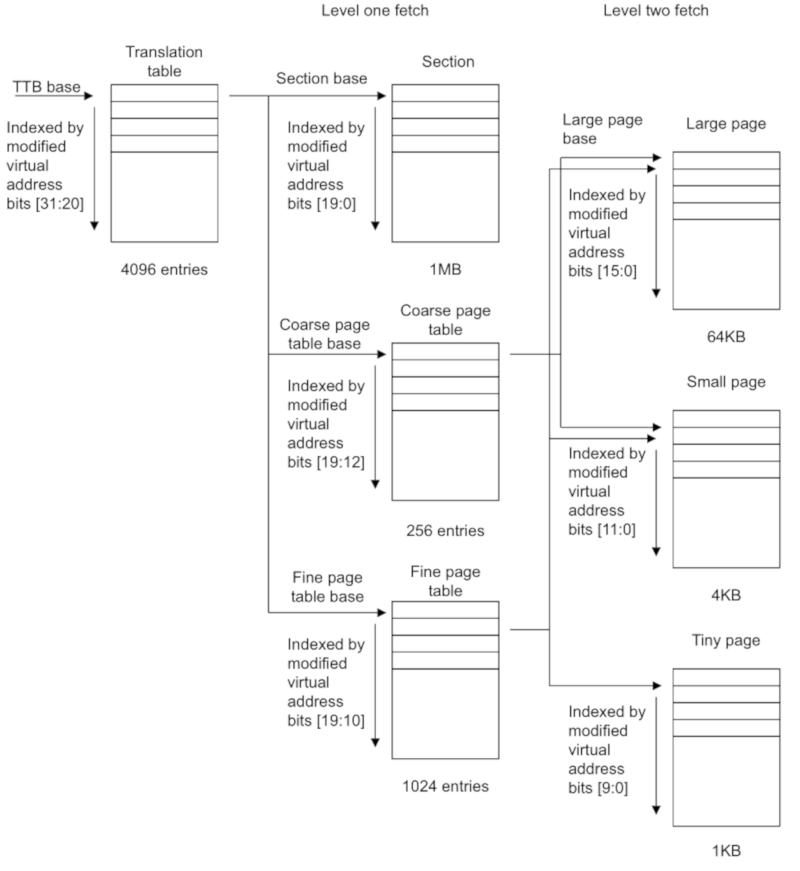
\includegraphics[height = 0.9\textheight]{arm_addr_transl}
%     \caption{Трансляция адресного пространства на ARMv5+
%       процессорах}\label{fig:armv5_addr_transl}
%   \end{figure}

%   \note{

%     Что касается ARM архитектуры, то там складывается похожая картина. Есть
%     несколько отличий: используются \textbf{отображения других размеров} (1MB
%     --- секции, 64KB --- большие страницы, 4KB --- маленькие страницы и 1KB ---
%     крошечные страницы, на поздних версиях большего размера); используется
%     регистр \texttt{c2} (часть \texttt{CP15} регистров) (\textbf{Translation
%       Table Base Register TTBR}) для получения указателя на таблицу в физическом
%     адресном пространстве, содержащую описания секции или страницы (или и того и
%     другого); в отличии от Intel используется \textbf{двухуровневая трансляция}
%     (см. рисунок \ref{fig:armv5_addr_transl}) и другие.

%     На современных ARM процессорах (Cortex-A) используется два регистра для
%     хранения физического адреса таблицы трансляции адресов (\texttt{TTBR0} и
%     \texttt{TTBR1}). Обычно один из них используется для
%     \textbf{пользовательского пространства}, а другой для \textbf{пространства
%       адресов ядра}. Это может служит причиной, почему некоторые атаки работают
%     на x86-64 процессорах, но \textbf{не работают на ARM}. При попытке доступа
%     из пользовательского контекста выполнения к регистру, который отвечает за
%     адресацию в ядерном пространстве, возникает исключение.

%   }

% \end{frame}


% ------------------------------------------------------------------------------

\section{Basic attacks}
\subsection{Cache attacks}
\begin{frame}{\insertsubsection}

  \begin{figure}[h]
    \begin{tikzpicture}[
      align = center,
      ->,
      > = Stealth,
      thick,
      block/.style = {
        draw,
        fill = ForestGreen,
        text = White,
      },
      ]

      \node[
      block,
      label = above:Кэш,
      minimum width = 1cm,
      minimum height = 1cm,
      ] (cache) {
        Данные
      };

      \node[
      block,
      label = above:DRAM,
      below = of cache,
      minimum width = 3cm,
      minimum height = 3cm,
      ] (dram) {
        Данные
      };

      \node[
      block,
      right = 3cm of $(cache.east)!.5!(dram.east)$,
      minimum width = 2cm,
      minimum height = 2cm,
      ] (cpu) {
        CPU
      };

      \draw (cpu) -> node[above, sloped] {0.5 ns -- 7 ns} (cache);
      \draw (cpu) -> node[below, sloped] {250 ns} (dram);

    \end{tikzpicture}
    \caption{Кэш --- это не только полезно, но и опасно}\label{cache_faster}
  \end{figure}

  \note{

    Главное \textbf{предназначение кэш--памяти} --- \textbf{нивелировать
      задержки} при работе с медленной главной физической памятью. При работе с
    данными через кэш задержки значительно уменьшаются. Kocher в 1996 году
    описал возможность использования разницы во времени при обращении к данным
    для совершения атаки, которая стала называться \textbf{атака на кэш по
      времени}.

  }
\end{frame}


\begin{frame}{\insertsubsection}

  \begin{figure}[h]
    \begin{tikzpicture}[
      align = center,
      ->,
      > = Stealth,
      thick,
      block/.style = {
        draw,
        fill = ForestGreen,
        text = White,
      },
      ]

      \node[
      block,
      label = above:Кэш,
      minimum width = 1cm,
      minimum height = 1cm,
      ] (cache) {
        Данные
      };

      \node[
      block,
      right = 3cm of cache,
      minimum width = 2cm,
      minimum height = 2cm,
      ] (cpu) {
        CPU
      };

      \draw (cpu) -> node[above] {
        
\includegraphics[height = .1\textheight]{hourglass} = ?
      } (cache);

    \end{tikzpicture}
    \caption{Для атаки на кэш необходимо знать точное время цикла обращения к
      ячейке памяти}\label{cache_time_attack}
  \end{figure}

  \note{

    Для проведения успешной кеш-атаки необходимо \textbf{знать точное время
      цикла обращения к ячейке памяти}. Ранние кеш--атаки использовали для этих
    целей \textbf{системные счётчики производительности}, но этот способ
    \textbf{неэффективен}, поскольку эти счётчики на ARM-процессорах доступны
    только в привилегированном режиме.

    Однако в 2016 году были предложены \textbf{три альтернативных источника}
    синхронизации, доступные в том числе и в непривилегированном режиме. Один из
    них --- запуск \textbf{параллельного синхронизирующего потока}, который
    непрерывно инкрементирует глобальную переменную. Читая значение этой
    переменной, злоумышленник может измерять время цикла обращения к ячейке
    памяти. Об остальных методах \textbf{будет рассказано позже} в ходе
    повествования.

    Кроме того, в \textbf{ARM--процессорах} действует так называемая политика
    псевдослучайного замещения, в результате действия которой,
    \textbf{вытеснение из кеша происходит менее предсказуемо}, чем в процессорах
    Intel и AMD. Тем не менее в 2016 году была \textbf{продемонстрирована
      эффективная кеш-атака} даже в таких зашумленных условиях.

  }
\end{frame}

\subsubsection{Evict + Time}
\begin{frame}{\insertsubsubsection}

  \begin{enumerate}
  \item Измерить время выполнения программы--жертвы
  \item Вытеснить определённый набор кэша
  \item Снова измерить время выполнения программы--жертвы и сравнить
  \end{enumerate}

  \note{

    Атакующий запускает несколько вычислений и затем измеряет время,
    потребовавшееся на завершение данных вычислений. Для определения влияния на
    конкретный набор кэша, атакующий предварительно вытесняет этот набор перед
    вторым запуском вычислений. Для второй половины запусков вычислений
    атакующий производит сравнение времени, и в случае, если время вычислений
    изменилось, значит именно этот набор кэша использовался для вычислений.

  }

\end{frame}

\begin{frame}{\insertsubsubsection}

  \only<1>{Измерить время выполнения программы--жертвы}

  \only<2,4>{Вытеснить определённый набор кэша}

  \only<3,5>{Снова измерить время выполнения программы--жертвы и сравнить}

  \begin{figure}[h]

  \newcommand*\viccolor{ForestGreen}
  \newcommand*\attcolor{White}
  \newcommand*\attcolorone{White}

  \only<4,5>{
    \renewcommand*\viccolor{BrickRed}
  }
  \only<2,3>{
    \renewcommand*\attcolor{NavyBlue}
  }

  \only<4,5>{
    \renewcommand*\attcolorone{NavyBlue}
  }

    \begin{tikzpicture}[
      align = center,
      ->,
      > = Stealth,
      thick,
      ampersand replacement = \&,
      block/.style = {
        draw,
        fill = ForestGreen,
        text = White,
      },
      cache/.style = {
        matrix of nodes,
        nodes in empty cells,
        nodes = {
          minimum width = .5cm,
          minimum height = .5cm,
          draw,
          align = center,
          anchor = center,
        },
      },
      ]

      \node<1,3,5>[
      font = \ttfamily,
      text = Black,
      align = left,
      ] (victim) {
        long long *rsa\_encrypt(...)
        \{\\
          $\cdots$\\
          for (i = 0; i < size; i++)\{\\
            encrypted[i] = rsa\_modExp(\\
              message[i],\\
              pub->exponent,\\
              pub->modules);\\
          \}\\
          $\cdots$\\
        \}\\
      };

      \node<1,3,5>[
      above = .1 of victim,
      ] (time) {
        \only<1>{0.30 ms}
        \only<3>{0.28 ms}
        \only<5>{0.56 ms}
      };

      \node[
      cache,
      right = of victim,
      label = {Кэш (8 наборов, 4 пути)},
      ] (cache) {
        \node[fill = ForestGreen] {}; \& \& \& \\
         \& \& \& \\
         \& \& \node[fill = ForestGreen] {}; \& \\
         \& \& \& \\
         \& \node[fill = ForestGreen] {}; \& \& \node[fill = ForestGreen] {}; \\
         \& \& \& \\
        \node[fill = \attcolorone] (attack_1) {}; \& \node[fill = \attcolorone] {}; \& \node[fill = \viccolor] (detect) {}; \& \node[fill = \attcolorone] {}; \\
        \node[fill = \attcolor] (attack_0) {}; \& \node[fill = \attcolor] {}; \& \node[fill = \attcolor] {}; \& \node[fill = \attcolor] {}; \\
      };

      \node<2,4,5>[
      left = of cache,
      ] (bsd) {
        
\includegraphics[height = .1\textheight]{freebsd}
      };

      \draw<2>[red] (bsd) -> (attack_0.west);
      \draw<4>[red] (bsd) -> (attack_1.west);
      \draw<5>[red] (bsd) -> (detect.center);

    \end{tikzpicture}
    % \caption{Пример атаки Evict + Time}\label{evict_time_example}
  \end{figure}

  \note<1>{

    \textbf{Кэш должен быть прогретым.}

  }

  \note<5>{

    \texttt{Evict + Time} метод даёт детальную информацию об используемом наборе
    кэша, но \textbf{«шум»}, получаемый от других источников, мешает корректно
    вычислить время исполнения задачи. По этой причине может потребоваться
    \textbf{несколько тысяч повторений запусков} для получения, например, целого
    AES ключа. Данный метод требует от атакующего возможности \textbf{точного
      измерения времени начала и окончания вычислений}. Это может оказаться
    \textbf{неосуществимым} в случае выполнения атаки \textbf{асинхронно}, так
    как атакующий не имеет возможности запускать вычисления по своему
    усмотрению. Преимущество \texttt{Evict + Time} метода в том, что ему
    \textbf{не требуется работать с разделяемой памятью}.

    \textbf{Усложнённые адресация данных и правила вымещения из кэша} на
    современных процессорах делает этап очищения данных из набора кэша сложнее
    и, соответственно, саму атаку с помощью метода \texttt{Evict + Time}.

  }
\end{frame}

\subsubsection{Prime + Probe}
\begin{frame}{\insertsubsubsection}
  \begin{enumerate}
    \item Заполнить определённые наборы кэша
    \item Передать управление программе--жертве
    \item Определить какие наборы кэша всё ещё заполнены нашими данными
  \end{enumerate}

  \note{

    Вторая техника атаки представленная Osvik'ом оказалось более мощной.
    Атакующий в течении времени заполняет (primes) набор кэша, а затем измеряет
    как долго происходит повторный доступ к этим данным.

    Первое применение атаки было \textbf{нацелено на L1 кэш}. Однако,
    \textbf{обратная разработка} работы \textbf{кэшей последнего уровня} открыла
    возможность проведения атаки и на данный вид кэшей (2009). Существует
    множество примеров успешной атаки на криптографические алгоритмы из состава
    всё того же OpenSSL.

    2011 --- был представлен пример атаки на \textbf{соседние облака и
      прослушивание соседних виртуальных машин}. Однако, эти атаки были
    совершены на микроархитектуры \textbf{с простой организацией}, где
    отсутствовали срезы кэшей и сложные функции по вычислению адресов.

    Позже --- и на современные процессоры, в том числе атака на AES BouncyCastle
    (\textbf{ARM}), атака на \textbf{TrustZone}, \textbf{Intel SGX анклав}.

  }
\end{frame}

\begin{frame}{\insertsubsubsection}

  \only<1>{Заполнить определённые наборы кэша}

  \only<2>{Передать управление программе--жертве}

  \only<3-6>{Определить какие наборы кэша всё ещё заполнены нашими данными}

  \begin{figure}[h]

    \newcommand*\viccolor{White}
    \newcommand*\vicatcolorone{White}
    \newcommand*\vicatcolortwo{White}
    \newcommand*\attcolor{NavyBlue}
    \newcommand*\attcolorone{White}

    \only<1>{
      \renewcommand*\vicatcolorone{NavyBlue}
      \renewcommand*\vicatcolortwo{NavyBlue}
    }
    \only<2-7>{
      \renewcommand*\viccolor{ForestGreen}
    }
    \only<2-4>{
      \renewcommand*\vicatcolorone{ForestGreen}
    }
    \only<2-6>{
      \renewcommand*\vicatcolortwo{ForestGreen}
    }
    \only<4->{
      \renewcommand*\vicatcolorone{BrickRed}
    }
    \only<6->{
      \renewcommand*\vicatcolortwo{BrickRed}
    }

    \begin{tikzpicture}[
      align = center,
      ->,
      > = Stealth,
      thick,
      ampersand replacement = \&,
      block/.style = {
        draw,
        fill = ForestGreen,
        text = White,
      },
      cache/.style = {
        matrix of nodes,
        nodes in empty cells,
        nodes = {
          minimum width = .5cm,
          minimum height = .5cm,
          draw,
          align = center,
          anchor = center,
        },
      },
      caption/.style = {
        fill = White,
        sloped,
        above,
        inner sep = 0,
        outer sep = 3,
      },
      ]

      \node[
      cache,
      label = {Кэш (8 наборов, 4 пути)},
      ] (cache) {
        \&\&\&\\
        \& \node[fill = \viccolor] (vic_0) {}; \&\&\\
        \&\&\&\\
        \&\&\&\\
        \&\&\&\\
        \& \node[fill = \viccolor] (vic_1) {}; \& \node[fill = \viccolor] (vic_2) {}; \&\\
        \&\&\&\\
        \node[fill = \attcolor] (att_0) {}; \& \node[fill = \vicatcolorone] (vic_3) {}; \& \node[fill = \attcolor] (att_1) {}; \& \node[fill = \vicatcolortwo] (vic_4) {}; \\
      };

      \node[
      left = of cache,
      ] (bsd) {
        
\includegraphics[height = .1\textheight]{freebsd}
      };

      \node[
      right = of cache,
      ] (smile) {
        
\includegraphics[height = .1\textheight]{smile}
      };

      \node<7>[
      right = of cache,
      yshift = 5,
      ] (aim) {
        
\includegraphics[height = .1\textheight]{aim}
      };

      \draw<1>[red] (bsd) -> (att_0.west);
      \draw<2>[LimeGreen] (smile) -> (vic_0.center);
      \draw<2>[LimeGreen] (smile) -> (vic_1.center);
      \draw<2>[LimeGreen] (smile) -> (vic_2.center);
      \draw<2>[LimeGreen] (smile) -> (vic_3.center);
      \draw<2>[LimeGreen] (smile) -> (vic_4.center);
      \draw<3>[red] (bsd) -> node[caption] {hit} (att_0.center);
      \draw<4>[red] (bsd) -> node[caption] {miss} (vic_3.center);
      \draw<5>[red] (bsd) -> node[caption] {hit} (att_1.center);
      \draw<6>[red] (bsd) -> node[caption] {miss} (vic_4.center);
      \draw<7>[red] (bsd) -> node[caption] {Detected!} (att_0.west);

    \end{tikzpicture}
    % \caption{Пример атаки Prime + Probe}\label{prime_probe_example}
  \end{figure}

  \note<1> {

    Атака проиллюстрирована в трёх шагах. Атакующий непрерывно заполняет набор
    кэша, используя доступ к своей памяти и позднее измеряет время доступа (шаг
    1 и 3).

  }

  \note<2>{

    На шаге 2 жертва, возможно, обращается к участку памяти (не общей), которая
    расположена в том же наборе кэша.

  }

  \note<3-6>{

    Если жертва обращалась в тот же набор кэша, то время доступа к данным на
    шаге 3 увеличится, так как один из путей кэша будет заменён, в противном
    случае время доступа будет меньше.

    \textbf{Время}, затрачиваемое на повторный доступ к набору кэша
    \textbf{пропорционально количеству путей}, которые были заменены другими
    процессами. \textbf{Большое время} при измерении означает, что \textbf{по
      крайней мере один путь кэша был заменён}, и наоборот --- меньшее время
    указывает на то, что ни один из путей кэша не был заменён.

  }

  \note<7>{

    Атака имеет такую же \textbf{детализацию} направленности атаки, как и Evict
    + Time атака, т. е. \textbf{набор кэша}. \textbf{Точность атаки больше}, чем
    в случае с Evict + Time, так как измеряется время \textbf{прямого доступа к
      данным}, а Evict + Time измеряет время через запуски вычислений, а не
    напрямую. Но также, как и с Evict + Time атакой, \textbf{усложнение функций
      адресации и правил вымещения} из кэша делает проведение атаки
    затруднительным.

  }

\end{frame}

\subsubsection{Flush + Reload}
\begin{frame}{\insertsubsubsection}
  \begin{enumerate}
  \item Отобразить бинарный файл (например, разделяемый объект) в своё адресное
    пространство
  \item Сбросить содержимое кэш--линии (код или данные)
  \item Передать управление программе--жертве
  \item Определить какие линии кэша были загружены программой--жертвой снова
  \end{enumerate}

  \note{

    Данная атака считается \textbf{наиболее эффективной} атакой на кэш. Целью
    данной атаки является не просто набор кэша, а \textbf{отдельная линия кэша},
    более того, у атакующего существует возможность проверить закэширована ли та
    или иная область памяти. Атака \texttt{Flush + Reload} выполняется в три
    фазы.

  }
\end{frame}

\begin{frame}{\insertsubsubsection}

  \only<1>{Отобразить бинарный файл (например, разделяемый объект) в своё
    адресное пространство}%

  \only<2>{Сбросить содержимое кэш--линии (код или данные)}%

  \only<3>{Передать управление программе--жертве}%

  \only<4>{Определить какие линии кэша были загружены программой--жертвой
    снова}%

  \begin{figure}[h]

    \newcommand*\viccolor{ForestGreen}
    \newcommand*\vicatcolorone{ForestGreen}
    \newcommand*\vicatcolortwo{ForestGreen}
    \newcommand*\attcolor{NavyBlue}
    \newcommand*\attcolorone{White}

    \only<2>{
      \renewcommand*\vicatcolorone{White}
      \renewcommand*\vicatcolortwo{White}
    }
    \only<3>{
      \renewcommand*\vicatcolorone{White}
      \renewcommand*\vicatcolortwo{ForestGreen}
    }
    \only<4->{
      \renewcommand*\vicatcolorone{NavyBlue}
      \renewcommand*\vicatcolortwo{BrickRed}
    }

    \begin{tikzpicture}[
      align = center,
      ->,
      > = Stealth,
      thick,
      ampersand replacement = \&,
      block/.style = {
        draw,
        fill = ForestGreen,
        text = White,
      },
      cache/.style = {
        matrix of nodes,
        nodes in empty cells,
        nodes = {
          minimum width = .5cm,
          minimum height = .5cm,
          draw,
          align = center,
          anchor = center,
        },
      },
      caption/.style = {
        fill = White,
        sloped,
        above,
        inner sep = 0,
        outer sep = 3,
      },
      ]

      \node[
      cache,
      label = {Кэш (8 наборов, 4 пути)},
      ] (cache) {
        \& \& \& \\
        \& \node[fill = \vicatcolorone] (vic_0) {}; \& \& \\
        \& \& \& \\
        \& \& \node[fill = \vicatcolortwo] (vic_1) {}; \& \\
        \& \& \& \\
        \& \& \& \\
        \& \& \& \\
        \& \& \& \\
      };

      \node[
      left = of cache,
      ] (bsd) {
        
\includegraphics[height = .1\textheight]{freebsd}
      };

      \node[
      right = of cache,
      ] (smile) {
        
\includegraphics[height = .1\textheight]{smile}
      };

      \node<5>[
      right = of cache,
      yshift = 5,
      ] (aim) {
        
\includegraphics[height = .1\textheight]{aim}
      };

      \draw<1>[Green] (smile) -> (vic_0);
      \draw<1>[Green] (smile) -> (vic_1);
      \draw<1>[red] (bsd) -> (vic_0);
      \draw<1>[red] (bsd) -> (vic_1);
      \draw<2>[red] (bsd) -> node[caption] {flush} (vic_0);
      \draw<2>[red] (bsd) -> node[caption] {flush} (vic_1);
      \draw<3>[Green] (smile) -> (vic_1);
      \draw<4>[red] (bsd) -> node[caption] {miss} (vic_0);
      \draw<4>[red] (bsd) -> node[caption] {hit} (vic_1);
      \draw<5>[red] (bsd) -> node[caption] {Detected!} (vic_1);

    \end{tikzpicture}
    % \caption{Пример атаки Flush + Reload}\label{flush_reload_example}
  \end{figure}

  \note<1>{

    \texttt{Flush + Reload} атака работает при условии \textbf{общей памяти},
    ярким примером может служить общая библиотека, которую использует и
    атакующий и программа--жертва. По этой причине, в случае, если нет такого
    элемента, как общая память между атакующим и жертвой, придётся использовать
    схему атаки \texttt{Prime + Probe}.

  }

  \note<2>{

    Во время первой фазы контролируемый участок памяти удаляется из структуры
    кэша (удаляется линия кэша с помощью инструкции \textbf{clflush} в случае с
    Intel).

  }


  \note<3>{

    Во второй фазе программа--шпион находится в режиме ожидания, \textbf{давая
      жертве время воспользоваться} участком памяти.

  }

  \note<4>{

    Во время третьей фазы программа--шпион \textbf{перезагружает} участок памяти
    и \textbf{замеряет время} загрузки. Если во время второй фазы жертва
    \textbf{воспользовалась} участком памяти, то этот участок будет доступен из
    кэша и операция перезагрузки \textbf{пройдёт быстро}. С другой стороны, если
    линия кэша \textbf{осталась неиспользованной}, понадобится время на загрузку
    участка и операция перезагрузки пройдёт \textbf{значительно дольше}.

  }


  \note<5>{

    Такие методы атаки, как \texttt{Flush + Reload} и \texttt{Flush + Flush}
    (описан ниже), используют \textbf{непривилегированную} x86--инструкцию
    сброса \texttt{clflush} для удаления строки данных из кеш--памяти. Однако,
    за исключением процессоров ARMv8-A, \textbf{ARM--платформы не имеют
      непривилегированных инструкций сброса кеша}, и поэтому в 2016 году был
    предложен \textbf{косвенный метод вытеснения кеша}, с использованием эффекта
    Rowhammer.

  }
\end{frame}

\subsubsection{Flush + Flush}
\begin{frame}{\insertsubsubsection}

  \begin{figure}[h]
    \begin{tikzpicture}[
      align = center,
      ->,
      > = Stealth,
      thick,
      ampersand replacement = \&,
      block/.style = {
        draw,
        fill = ForestGreen,
        text = White,
      },
      cache/.style = {
        matrix of nodes,
        nodes in empty cells,
        nodes = {
          minimum width = .5cm,
          minimum height = .5cm,
          draw,
          align = center,
          anchor = center,
        },
      },
      caption/.style = {
        fill = White,
        sloped,
        above,
        inner sep = 0,
        outer sep = 3,
      },
      ]

      \node[
      cache,
      label = {Кэш (8 наборов, 4 пути)},
      ] (cache) {
        \& \& \& \\
        \& \node[fill = ForestGreen] (vic_0) {}; \& \& \\
        \& \& \& \\
        \& \& \node[fill = ForestGreen] (vic_1) {}; \& \\
        \& \& \& \\
        \& \& \& \\
        \& \& \& \\
        \& \& \& \\
      };

      \node[
      left = of cache,
      ] (bsd) {
        
\includegraphics[height = .1\textheight]{freebsd}
      };

      \node[
      right = of cache,
      text = Black,
      label = {[White] below:Я слежу за тобой!},
      ] (smile) {
        
\includegraphics[height = .1\textheight]{smile}
      };

      \draw[red] (bsd) -> (vic_0);
      \draw[red] (bsd) -> (vic_1);
      \draw[red] (bsd) -> (cache-1-1.center);
      \draw[red] (bsd) -> (cache-1-2.center);
      \draw[red] (bsd) -> (cache-3-1.center);
      \draw[red] (bsd) -> (cache-5-3.center);
      \draw[red] (bsd) -> (cache-6-1.center);
      \draw[red] (bsd) -> (cache-7-2.center);

    \end{tikzpicture}
    \caption{Количество и продолжительность обращений к памяти может быть
      измерено, а атаки на кэш --- обнаружены}\label{cache_attacks_detection}
  \end{figure}

  \note{

    Атаки типа \texttt{Flush + Reload} и \texttt{Prime + Probe} производят
    \textbf{большое количество обращений} к памяти, продолжительность которых
    \textbf{можно измерить} (при помощи системных счётчиков производительности),
    по этой причине они \textbf{могут быть опознаны} процессором.

    Атака \textbf{Flush + Flush} представляет из себя \textbf{стелс--версию}
    атаки \texttt{Flush + Reload}.

  }

\end{frame}

\begin{frame}{\insertsubsubsection}

  \begin{figure}[h]

    \begin{tikzpicture}[
      align = center,
      ->,
      > = Stealth,
      thick,
      ampersand replacement = \&,
      block/.style = {
        draw,
        fill = ForestGreen,
        text = White,
      },
      cache/.style = {
        matrix of nodes,
        nodes in empty cells,
        nodes = {
          minimum width = .5cm,
          minimum height = .5cm,
          draw,
          align = center,
          anchor = center,
        },
      },
      caption/.style = {
        fill = White,
        sloped,
        above,
        inner sep = 0,
        outer sep = 3,
      },
      ]

      \node[
      cache,
      label = {Кэш (8 наборов, 4 пути)},
      ] (cache) {
        \& \& \& \\
        \& \node[fill = ForestGreen] (vic_0) {}; \& \& \\
        \& \& \& \\
        \& \& \node[fill = ForestGreen] (vic_1) {}; \& \\
        \& \& \& \\
        \& \& \& \\
        \& \& \& \\
        \& \& \& \\
      };

      \node[
      left = of cache,
      ] (bsd) {
        
\includegraphics[height = .1\textheight]{freebsd}
      };

      \draw[red] (bsd) -> node[caption, text = BlueViolet] {3.83ns} (vic_0);
      \draw[red] (bsd) -> node[caption, text = BlueViolet] {4.85ns} (vic_1);
      \draw[red] (bsd) -> node[caption, text = Black] {0.96ns} (cache-7-4.center);
      \draw[red] (bsd) -> node[caption, text = Black] {1.06ns} (cache-8-1.center);

    \end{tikzpicture}
    \caption{Инструкция для сброса кэша срабатывает за различное время в
      зависимости от того, находятся ли сейчас какие-либо данные в кэше или
      нет}\label{flush_flush_example}
  \end{figure}

  \note{

    Было выяснено, что \textbf{инструкция для сброса кэша срабатывает за
      различное время} в зависимости от того, находятся ли сейчас какие-либо
    данные в кэше или нет. В случае, если данные, которые подвергаются
    вытеснению \textbf{присутствуют}, то вытеснение происходит
    \textbf{медленнее}. Таким образом вместо повторной загрузки данных в кэш,
    атакующий снова вытесняет кэш и также измеряет время.

  }
\end{frame}

\subsubsection{Evict + Reload}
\begin{frame}{\insertsubsubsection}

  \only<1>{Отобразить бинарный файл (например, разделяемый объект) в своё
    адресное пространство}

  \only<2>{Вытеснить содержимое кэш--линии (код или данные)}

  \only<3>{Передать управление программе--жертве}

  \only<4>{Определить какие линии кэша были загружены программой--жертвой снова}

  \begin{figure}[h]

    \newcommand*\viccolor{ForestGreen}
    \newcommand*\vicatcolorone{ForestGreen}
    \newcommand*\vicatcolortwo{ForestGreen}
    \newcommand*\attcolor{White}
    \newcommand*\attcolorone{White}

    \only<2>{
      \renewcommand*\vicatcolorone{NavyBlue}
    }
    \only<2->{
      \renewcommand*\attcolor{NavyBlue}
      \renewcommand*\vicatcolortwo{NavyBlue}
    }
    \only<3>{
      \renewcommand*\vicatcolorone{BrickRed}
      % \renewcommand*\vicatcolortwo{ForestGreen}
    }
    \only<4->{
      \renewcommand*\vicatcolorone{BrickRed}
      % \renewcommand*\vicatcolortwo{ForestGreen}
    }

    \begin{tikzpicture}[
      align = center,
      ->,
      > = Stealth,
      thick,
      ampersand replacement = \&,
      block/.style = {
        draw,
        fill = ForestGreen,
        text = White,
      },
      cache/.style = {
        matrix of nodes,
        nodes in empty cells,
        nodes = {
          minimum width = .5cm,
          minimum height = .5cm,
          draw,
          align = center,
          anchor = center,
        },
      },
      caption/.style = {
        fill = White,
        sloped,
        above,
        inner sep = 0,
        outer sep = 3,
      },
      ]

      \node[
      cache,
      label = {Кэш (8 наборов, 4 пути)},
      ] (cache) {
        \& \& \& \\
        \node[fill = \attcolor] (evict_0) {}; \& \node[fill = \vicatcolorone] (vic_0) {}; \& \node[fill = \attcolor] {}; \& \node[fill = \attcolor] {}; \\
        \& \& \& \\
        \node[fill = \attcolor] (evict_1) {}; \& \node[fill = \attcolor] {}; \& \node[fill = \vicatcolortwo] (vic_1) {}; \& \node[fill = \attcolor] {}; \\
        \& \& \& \\
        \& \& \& \\
        \& \& \& \\
        \& \& \& \\
      };

      \node[
      left = of cache,
      ] (bsd) {
        
\includegraphics[height = .1\textheight]{freebsd}
      };

      \node[
      right = of cache,
      ] (smile) {
        
\includegraphics[height = .1\textheight]{smile}
      };

      \node<5>[
      right = of cache,
      yshift = 5,
      ] (aim) {
        
\includegraphics[height = .1\textheight]{aim}
      };

      \draw<1>[green] (smile) -> (vic_0);
      \draw<1>[green] (smile) -> (vic_1);
      \draw<1>[red] (bsd) -> (vic_0);
      \draw<1>[red] (bsd) -> (vic_1);
      \draw<2>[red] (bsd) -> node[caption] {evict} (evict_0.west);
      \draw<2>[red] (bsd) -> node[caption] {evict} (evict_1.west);
      \draw<3>[green] (smile) -> (vic_0);
      \draw<4>[red] (bsd) -> node[caption] {hit} (vic_0);
      \draw<4>[red] (bsd) -> node[caption] {miss} (vic_1);
      \draw<5>[red] (bsd) -> node[caption] {Detected!} (vic_0);

    \end{tikzpicture}
    % \caption{Пример атаки Flush + Reload}\label{flush_reload_example}
  \end{figure}

  \note<1>{

    Атака представляет из себя \textbf{модифицированную версию Flush + Reload} и
    имеет смысл для архитектур, где \textbf{инструкция вытеснения} из кэша
    доступна \textbf{только в привилегированном режиме}, например, для ARM.

  }

  \note<2>{

    Суть атаки заключается в том, что \textbf{для вытеснения} нужной линии кэша
    происходит \textbf{заполнение кэш--памяти большим количеством
      взаимосвязанных адресов}, в результате чего механизм, отвечающий за
    вытеснение, сам начнёт вытеснять нужную нам линию кэша.

  }

  \note<5>{

    Новый (2017 год) тип атаки на кэш от
    \href{https://www.vusec.net/projects/anc/}{Systems and Network Security
      Group at VU Amsterdam}.

    Атака представляет из себя \textbf{модифицированную версию Evict + Time}.
    Были использованы \textbf{новые методы для расчёт времени} (Time to Tick ---
    ввиду ограничений на стандартный счётчик, который теперь отсчитывает такты,
    не измеряя точное время доступа к памяти, отсчитываются такты после
    обращения к памяти; Shared Memory Counter --- параллельный счётчик на
    отдельном ядре; пример на рисунке \ref{fig:arc_new_timers}). Также
    \textbf{использовалась атака Prime + Probe} на MMU (Memory Management Unit),
    для возможности проведения атаки на кэш последнего уровня.

  }

\end{frame}

\subsection{Branch-prediction attacks}
\begin{frame}{\insertsubsection}

  \begin{figure}[h]
    \begin{tikzpicture}[
      align = center,
      ->,
      > = Stealth,
      thick,
      ampersand replacement = \&,
      block/.style = {
        draw,
        fill = ForestGreen,
        text = White,
      },
      cache/.style = {
        matrix of nodes,
        nodes in empty cells,
        inner sep = 0,
        nodes = {
          minimum width = 3cm,
          minimum height = .5cm,
          draw,
          align = center,
          anchor = center,
        },
      },
      ]

      \node[
      cache,
      label = {Branch Target Buffer},
      ] (btb) {
        Address tag \& Target \\
        \& \\
        \& \\
        0xebe45a82 \& ??? \\
        \& \\
        \& \\
        \& \\
      };

      \node[
      draw,
      left = 7cm of btb.north,
      label = above:Virtual address (user space),
      ] (addr_user) {
        0x0000 \color{ForestGreen}EBE45A82
      };

      \node[
      draw,
      below = 4cm of addr_user,
      label = below:Virtual address (kernel space),
      ] (addr_kernel) {
        0xFFFF \color{ForestGreen}EBE45A82
      };

      \node[
      left = of btb,
      block,
      minimum width = 1cm,
      minimum height = 1cm,
      label = left:Indexing\\function,
      ] (f) {
        f(x)
      };

      \draw (addr_user.east) -| (f.north);
      \draw (addr_kernel.east) -| (f.south);
      \draw (f) -> (btb.west);

    \end{tikzpicture}
    \caption{Branch Target Buffer addressing scheme in Haswell
      processor}\label{btb_tag}
  \end{figure}

  \note{

    \textbf{Буфер адресов перехода (branch target buffer, BTB)} кэширует
    информацию о ранее выбранных переходах выполнения для быстрого угадывания
    будущих. Кэш использует индексацию на \textbf{базе виртуального адресного
      пространства}, таким образом \textbf{атакующему не обязательно знать
      физический адрес} для выполнения атаки.

    \textbf{Атакующий заполняет буфер адресов перехода} путём выполнения
    последовательности различных переходов. Если жертва--программа будет
    выполнять ту ветвь, которой не было в кэше, то она добавится туда, вытеснив
    тем самым существующую запись. \textbf{Атакующий может вычислить} какая
    ветвь была вытолкнута из буфера по сравнительно \textbf{большому времени
      выполнения} этой ветви.

    Пример атаки позволяет взломать KASLR из пользовательского процесса.
    Основывается на возникающих \textbf{коллизиях} в кэше branch target buffer.
    По времени выполнения своего кода атакующий имеет возможность
    \textbf{вычислить адрес перехода в ядерном пространстве} (значение берётся
    из BTB), тем самым вычислить смешение, полученное в результате KASLR.

    Возникает два типа коллизий:

    \begin{enumerate}
    \item cross domain collisions --- user и kernel space;
    \item same domain collisions --- разные user-space процессы, позволяет
      выявить смещения для ASLR другого процесса.
    \end{enumerate}

  }

\end{frame}

\subsection{TLB-based attacks}
\begin{frame}{\insertsubsection}

  \begin{figure}[h]

    \begin{tikzpicture}[
      align = center,
      ->,
      > = Stealth,
      ampersand replacement = \&,
      block/.style = {
        draw = dGreen,
      },
      ]

      \node[
      block,
      ] (tlb) {TLB};

      \node[
      left = of tlb,
      ] (virt_addr) {Virtual\\ Address};

      \node[
      below = of tlb,
      ] (hit) {Mapped address\\ returns quicker!};

      \node[
      block,
      label = above:\color{dBlue}Translation table,
      right = 6cm of tlb,
      rectangle split,
      rectangle split parts = 5,
      rectangle split empty part width = 1cm,
      ] (table) {%
        PML4E%
        \nodepart{two}%
        PDPTE%
        \nodepart{three}%
        PDE%
        \nodepart{four}%
        PTE%
        \nodepart{five}%
        Physical address%
      };

      \draw (virt_addr) -> (tlb);
      \draw (tlb) -> node[right] {\color{dGreen}Hit} (hit);

      \draw (tlb) -> node[below] {\color{dRed}Miss}
        node[above] {Unmapped address\\takes $\approx$ 40 cycles\\%
        more for page table walk} (table);

    \end{tikzpicture}
    \caption{A translation lookaside buffer (TLB) is a memory cache that is used
      to reduce the time taken to access a user memory
      location}\label{tlb_example}
  \end{figure}

  \note{

    Трансляция адресов должна происходить очень быстро. С использованием таблиц
    трансляций, расположенных в памяти, данная операция быстро выполняться не
    может. По этой причине был введён кеш для трансляции адресов, который
    помогает уменьшить задержку при процессе трансляции --- \textbf{буфер
      ассоциативной трансляции (translation lookaside buffer, TLB)}.

    Атака впервые была представлена Ralf Hund \textbf{в 2013 году}. Попытка
    чтения или записи памяти, к которой нет доступа по причине того, что данный
    участок памяти \textbf{используется ядром, занимает меньше времени}, если бы
    память не была размечена вовсе, т. к. используемые адреса памяти попадают в
    кэш независимо от уровня привилегий.

    Это позволяет узнать, какие адреса используются, и более того, узнать какие
    адреса \textbf{используются той или иной частью ядра}, т. е. данный вид
    атаки позволяет обойти технику рандомизации памяти в ядерном пространстве
    (kernel address-space-layout randomization, \textbf{KASLR}).

  }
\end{frame}


\subsection{Exception-based attacks}
\begin{frame}{\insertsubsection}

  \begin{itemize}
  \item прерывание планировщика
  \item инструкции прерывания
  \item ошибка отсутствия страницы в памяти
  \item поведенческие изменения (например, возврат кода ошибки)
  \end{itemize}

  \note{

    Данного рода атаки получают необходимую информацию из исключительных
    ситуаций, которые происходят при работе процессора. Обычными для процессора
    исключительными ситуациями являются: прерывание планировщика, прерывания
    инструкции, ошибка страницы памяти, а также поведенческие изменения,
    например, инструкции предоставляют пользователю код ошибки.

    Во время возникновения исключительных ситуаций можно получить информацию о
    работе процессора либо \textbf{напрямую} (основываясь на поведении самого
    процессора), либо \textbf{косвенно (через измерения времени, при
      возникновении исключительных ситуаций)}.

    Одним из ярких примеров атак подобного рода является \textbf{атака на
      систему дедупликации памяти}.

  }
\end{frame}

% \subsubsection{Атаки на систему дедупликации памяти}
% \begin{frame}{\insertsubsubsection}

%   \begin{figure}[h]

%     \begin{tikzpicture}[
%       align = center,
%       ->,
%       > = Stealth,
%       thick,
%       ampersand replacement = \&,
%       block/.style = {
%         draw,
%         fill = ForestGreen,
%         text = White,
%       },
%       block_split/.style = {
%         rectangle,
%         rectangle split,
%         rectangle split parts = 7,
%         rectangle split empty part width = 1cm,
%         draw,
%         text centered,
%         font = \scriptsize,
%       },
%       ]

%       \node[
%       block_split,
%       label = above:Виртуальная\\память 1,
%       rectangle split part fill = {
%         White, White, White, ForestGreen, White,
%         ForestGreen, White
%       },
%       ] (virt_0) {
%         \nodepart{two}
%         \nodepart{three}
%         \nodepart{four}
%         \nodepart{five}
%         \nodepart{six}
%         \nodepart{seven}
%         \nodepart{eight}
%       };

%       \node<3-4>[
%       block_split,
%       label = above:Физическая\\память,
%       right = 2cm of virt_0,
%       rectangle split part fill = {
%         White, White, White, White, ForestGreen,
%         White, ForestGreen
%       },
%       ] (phys) {
%         \nodepart{two}
%         \nodepart{three}
%         \nodepart{four}
%         \nodepart{five}
%         \nodepart{six}
%         \nodepart{seven}
%         \nodepart{eight}
%       };


%       \node<3-4>[
%       block_split,
%       label = above:Разделяемая\\физическая память,
%       right = 2cm of phys,
%       rectangle split part fill = {
%         White, ForestGreen, White, White, Blue,
%         White, White
%       },
%       ] (dedup) {
%         \nodepart{two}
%         \nodepart{three}
%         \nodepart{four}
%         \nodepart{five}
%         \nodepart{six}
%         \nodepart{seven}
%         \nodepart{eight}
%       };

%       \node<3-4>[
%       block_split,
%       label = above:Виртуальная\\память 2,
%       right = 2cm of dedup,
%       rectangle split part fill = {
%         ForestGreen, White, White, ForestGreen, White,
%         White, White
%       },
%       ] (virt_1) {
%         \nodepart{two}
%         \nodepart{three}
%         \nodepart{four}
%         \nodepart{five}
%         \nodepart{six}
%         \nodepart{seven}
%         \nodepart{eight}
%       };

%       \node<1-2>[
%       block_split,
%       label = above:Разделяемая\\физическая память,
%       right = 3cm of virt_0,
%       rectangle split part fill = {
%         White, ForestGreen, White, White, Blue,
%         White, ForestGreen
%       },
%       ] (phys) {
%         \nodepart{two}
%         \nodepart{three}
%         \nodepart{four}
%         \nodepart{five}
%         \nodepart{six}
%         \nodepart{seven}
%         \nodepart{eight}
%       };

%       \node<1-2>[
%       block_split,
%       label = above:Виртуальная\\память 2,
%       right = 3cm of phys,
%       rectangle split part fill = {
%         ForestGreen, White, White, ForestGreen, White,
%         White, White
%       },
%       ] (virt_1) {
%         \nodepart{two}
%         \nodepart{three}
%         \nodepart{four}
%         \nodepart{five}
%         \nodepart{six}
%         \nodepart{seven}
%         \nodepart{eight}
%       };

%       \draw<1-2> (virt_0.four east) -> (phys.five west);
%       \draw<1-2> (virt_0.six east) -> (phys.seven west);
%       \draw<1-2> (virt_1.four west) -> (phys.five east);
%       \draw<1-2> (virt_1.one west) -> (phys.two east);

%       \draw<2> (virt_0.four east) -> node[above, sloped] {Page fault!} node[below, sloped] {Запись} (phys.five west);

%       \draw<3> (virt_0.four east) -> (phys.five west);
%       \draw<3> (virt_0.six east) -> (phys.seven west);
%       \draw<3> (virt_1.four west) -> (dedup.five east);
%       \draw<3> (virt_1.one west) -> (dedup.two east);

%       \draw<4> (virt_1.four west) -> (dedup.five east);
%       \draw<4> (virt_1.one west) -> (dedup.two east);
%       \draw<4> (virt_0.four east) -> node[below, sloped] {Запись} node[above, sloped] {244ns} (phys.five west);
%       \draw<4> (virt_0.four west) -- ++(-1, 0) -- ++(0, -2) -- node[below] {Запись} node[above] {275ns} ++(7, 0) |- (dedup.five west);


%     \end{tikzpicture}
%     \only<1>{\caption{Дедупликация памяти}}\label{dedup_example}

%     \only<2>{\caption{Процесс 1 пытается записать данные в разделяемую память}}

%     \only<3>{\caption{Запись в дедуплицированную память происходит в режиме
%         Copy-on-Write}}
%   \end{figure}

%   \note<1>{

%     \textbf{Подсистема дедупликации} контент--ориентированных страниц
%     \textbf{сканирует всю системную память на идентичные физические} страницы
%     памяти и \textbf{склеивает их в одну} физическую страницу.

%   }

%   \note<2>{

%     Подсистема дедупликации проецирует несколько \textbf{идентичных копий
%       физических страниц} памяти \textbf{на одну} разделяемую копию, с доступом
%     в режиме \textbf{«копирование при записи»}. В результате при запросах на
%     чтение каждый процесс получает данные из одной и той же страницы. Если же
%     процесс хочет записать данные, то перед тем, как он сможет это сделать, для
%     него создаётся отдельная копия страницы. В результате \textbf{запись в
%       разделённую страницу вызывает «страничный отказ»}.

%   }

%   \note<4> {

%     Следовательно, \textbf{запись в разделяемую страницу происходит значительно
%       медленнее}, чем запись в обычную страницу. Злоумышленник,
%     \textbf{способный создавать страницы в целевой системе}, может использовать
%     эту разницу во времени, чтобы обнаружить факт \textbf{существования
%       интересующих его страниц}.

%   }

% \end{frame}

\subsection{DRAM-based attacks}
\begin{frame}{\insertsubsection}

  \begin{figure}[h]

    \newcommand*\dramcolor{White, White, White,
      White, White, White, White}

    \newcommand*\bufcolor{White}

    \only<2>{
      \renewcommand*\dramcolor{White, ForestGreen, White,
      White, White, White, White}
    }

    \only<3-5>{
      \renewcommand*\dramcolor{White, ForestGreen, White,
        White, White, White, White}
      \renewcommand*\bufcolor{ForestGreen}
    }

    \begin{tikzpicture}[
      align = center,
      ->,
      > = Stealth,
      thick,
      dram/.style = {
        rectangle,
        rectangle split,
        rectangle split parts = 7,
        rectangle split part fill = \dramcolor,
        minimum width = 3cm,
        draw,
        text = Black,
        text centered,
      },
      block/.style = {
        rectangle,
        draw,
        fill = ForestGreen,
        text = White,
        text centered,
      },
      ]

      \node[
      dram,
      label = above:DRAM банк,
      ] (dram) {
        0123456789
        \nodepart{two}
        1234567890
        \nodepart{three}
        2345678901
        \nodepart{four}
        3456789012
        \nodepart{five}
        4567890123
        \nodepart{six}
        5678901234
        \nodepart{seven}
        6789012345
        \nodepart{eight}
      };

      \node[
      draw,
      fill = ForestGreen,
      text = White,
      left = 3cm of dram,
      minimum width = 2cm,
      minimum height = 2cm,
      ] (cpu) {
        CPU
      };

      \node[
      below = .5 of dram,
      text = Black,
      fill = \bufcolor,
      draw,
      minimum width = 3cm,
      ] (buf) {
        row buffer
      };

      \draw<3> (dram.two east) -- ++(1, 0) |- node[right] {Открытие} (buf);

      \draw<4-5> (buf) -- (cpu);


    \end{tikzpicture}
    \only<1>{\caption{Работа DRAM (ещё раз)}}\label{fig:draw_row_buffer}

    \only<2>{\caption{CPU запрашивает на чтение строку №1}}

    \only<3>{\caption{DRAM открывает строку №1}}

    \only<4>{\caption{CPU читает строку №1 из буфера строки}}

    \only<5>{\caption{CPU снова запрашивает на чтение строку №1, которая уже
        есть в буфере строки, чтение происходит быстрее}}
  \end{figure}

  \note<1>{

    Ещё раз о том, как работает \textbf{row buffer}.

  }

  \note<5>{

    При попадании строки чтение данных происходит быстрее, при промахе строки
    --- медленнее, что похоже на поведение при работе с кэшем.

    Также существуют атаки непосредственно на DRAM (DRAM addressing,
    \textbf{DRAMA}). Атака при \textbf{промахе строки} похожа на атаку на кэш
    \textbf{Prime + Probe}, атака при \textbf{попадании строки} сравнима с
    атакой \textbf{Flush + Reload}. Оба типа атаки работают и при
    \textbf{отсутствии разделяемой памяти}. DRAMA эксплуатирует буфер строки
    DRAM, как будто это \textbf{кэш с прямым отображением используемый банком}.

    Во время подготовки атаки DRAMA применяли методы реверс-инжиниринга,
    основанные на подобном поведении DRAM, для того, чтобы \textbf{выявить
      местоположение и архитектуру банков}.

  }

\end{frame}

\subsubsection{Row hit атака (Flush + Reload)}
\begin{frame}{\insertsubsubsection}

  \begin{figure}[h]

    \newcommand*\dramcolor{Green, NavyBlue, ForestGreen, ForestGreen, White,
      White, White}

    \newcommand*\bufcolor{Green}

    \only<2>{
      \renewcommand*\bufcolor{NavyBlue}
    }

    \only<3>{
      \renewcommand*\bufcolor{Green}
    }

    \only<4>{
      \renewcommand*\bufcolor{NavyBlue}
    }

    \begin{tikzpicture}[
      align = center,
      ->,
      > = Stealth,
      thick,
      dram/.style = {
        rectangle,
        rectangle split,
        rectangle split parts = 7,
        rectangle split part fill = \dramcolor,
        minimum width = 3cm,
        draw,
        text = Black,
        text centered,
      },
      block/.style = {
        rectangle,
        draw,
        fill = ForestGreen,
        text = White,
        text centered,
      },
      ]

      \node[
      dram,
      label = above:DRAM банк,
      ] (dram) {
        0123456789
        \nodepart{two}
        1234567890
        \nodepart{three}
        2345678901
        \nodepart{four}
        3456789012
        \nodepart{five}
        4567890123
        \nodepart{six}
        5678901234
        \nodepart{seven}
        6789012345
        \nodepart{eight}
      };

      \node[
      draw,
      fill = ForestGreen,
      text = White,
      left = 3cm of dram,
      minimum width = 2cm,
      minimum height = 2cm,
      ] (cpu) {
        CPU
      };

      \node[
      below = .5 of dram,
      text = Black,
      fill = \bufcolor,
      draw,
      minimum width = 3cm,
      ] (buf) {
        \only<1>{0123456789}%
        \only<2>{1234567890}%
        \only<3>{0123456789}%
        \only<4>{1234567890}%
      };

      \draw<1> (dram.one east) -- ++(1, 0) |- node[right] {Открытие} (buf);
      \draw<1> (buf) -- node[below, sloped] {Медленно!} (cpu);

      \draw<2> (dram.two east) -- ++(1, 0) |- node[right] {Открытие} (buf);
      \draw<2> (buf) -- node[below, sloped] {Медленно!} (cpu);

      \draw<3> (dram.one east) -- ++(1, 0) |- node[right] {Открытие} (buf);

      \draw<4> (dram.two east) -- ++(1, 0) |- node[right] {Открытие} (buf);
      \draw<4> (buf) -- node[below, sloped] {Быстро\\при повторном\\обращении!} (cpu);

    \end{tikzpicture}
    \only<1>{\caption{Атакующий запрашивает строку №0, содержимое которой
        принадлежит атакующему}}

    \only<2>{\caption{Атакующий запрашивает строку №1, содержимое которой
        частично принадлежит и атакующему, и жертве}}

    \only<3>{\caption{Сбросим (вытесним) буфер и передадим управление
        программе--жертве}}

    \only<4>{\caption{В случае, если жертва обращалась к данному адресу, то это
        можно вычислить по времени повторного обращения}}
  \end{figure}

  \note<1>{

    В случае атаки при \textbf{попадании строки}, атакующий и жертва используют
    \textbf{одну и ту же строку} DRAM.

  }

  \note<3>{

    Атакующий загружает другую строку в буфер строки (тем самым закрывая
    открытую строку), что похоже на начало атаки \textbf{Flush + Reload}.

  }

  \note<4>{

    Если жертва \textbf{обращалась} к общей уже закрытой строке, то данная
    строка снова будет загружена в буфер строки, что выяснится позже при
    повторном обращении атакующего к этой строке (\textbf{время обращения будет
      меньше}).

  }

\end{frame}

\subsection{Covert channels}
\begin{frame}{\insertsubsection}

  \begin{figure}[h]
    \begin{tikzpicture}[
      align = center,
      ->,
      > = Stealth,
      ampersand replacement = \&,
      cache/.style = {
        rectangle split,
        rectangle split parts = 4,
        draw = dGray,
        minimum width = 2cm,
      },
      cpu/.style = {
        draw = dGray,
        minimum width = 2cm,
      },
      ]

      \node[
      cache,
      label = above:Cache 0,
      ] (cache_0) {};

      \node[
      cpu,
      right = 2 of cache_0,
      ] (cpu_0) {CPU 0};

      \node[
      cache,
      label = above:Cache 3,
      above = of cache_0,
      ] (cache_3) {};

      \node[
      cpu,
      right = 2 of cache_3,
      ] (cpu_3) {CPU 3};

      \node[
      cache,
      label = above:Cache 1,
      left = of cache_0,
      ] (cache_1) {};

      \node[
      cpu,
      left = 2 of cache_1,
      ] (cpu_1) {CPU 1};

      \node[
      cache,
      label = above:Cache 2,
      above = of cache_1,
      ] (cache_2) {};

      \node[
      cpu,
      left = 2 of cache_2,
      ] (cpu_2) {CPU 2};

      \draw (cpu_0) -- (cache_0);
      \draw (cpu_1) -- (cache_1);
      \draw (cpu_2) -- (cache_2);
      \draw (cpu_3) -- (cache_3);

      \draw[dGreen] (cache_0.three west) -- ++(-0.5, 0) |- (cache_3.four west);
      \draw[dRed] (cache_1.three east) -- ++(0.3, 0) |- (cache_3.one west);
      \draw[dGreen] (cache_2.one east) -- ++(0.1, 0) |- (cache_3.three west);
      \draw[dBlue] (cache_1.two west) -- ++(-0.5, 0) |- (cache_2.one west);

    \end{tikzpicture}
    \caption{Cross-core covert channels}\label{covert_attack_example}
  \end{figure}

  \note{

    Современные облачные системы часто имеют \textbf{несколько процессоров},
    установленных в материнскую плату с \textbf{мультисокетом}. Кэшы процессоров
    содержатся в когерентном состоянии с помощью \textbf{межпроцессорных
      протоколов, обеспечивающих когерентность}. Однако, это обеспечивает эффект
    \textbf{разделяемой кэш линии}.

    Кеш-атаки позволяют реализовать \textbf{высокопроизводительные межъядерные и
      межпроцессорные скрытые кеш-каналы} на современных смартфонах, используя
    \texttt{Flush+Reload}, \texttt{Evict+Reload} или \texttt{Flush+Flush}.
    Скрытый канал позволяет двум \textbf{непривилегированным приложениям}
    взаимодействовать друг с другом \textbf{без использования} каких-либо
    системных \textbf{механизмов передачи данных}. Благодаря этому можно
    вырваться из песочницы и обойти систему «ограниченных разрешений». В
    частности, на Android злоумышленник может использовать одно приложение,
    которое имеет \textbf{доступ к личным контактам} владельца устройства, для
    \textbf{отправки данных по скрытому каналу} другому приложению, имеющему
    доступ к \textbf{интернет}.

  }

\end{frame}

\begin{frame}{\insertsubsection}
  \begin{itemize}
  \item Cache-based covert channels (shared libraries)
  \item Row miss attack (DRAM)
  \item Thermal covert channels
  \item Radio covert channels
  \end{itemize}

  \note{

    Wu в 2012 и в 2014 годах обнаружил \textbf{разницу во времени при доступе к
      памяти}, возникающую из-за \textbf{задержки в шине памяти}, что позволяет
    наладить скрытый канал передачи данных между \textbf{близко расположенными
      виртуальными машинами}. В облаке Amazon EC2 был налажен канал скоростью
    13.5 КБ/c при 0.75 \% ошибок. В 2016 Inci также обнаружил задержку в шине
    памяти, позволяющую наладить канал в облаках Microsoft Azure.

    В 2017 году была представлена первая в своём роде реализация
    \textbf{скрытого канала, работающего по протоколу SSH}, с относительно
    высокой пропускной способностью (45 Кбит/с); эта реализация обеспечивает
    отказоустойчивые коммуникации между двумя виртуальными машинами даже в
    условиях экстремальной зашумлённости кеша.
    
    
  }
\end{frame}

% \subsubsection{Пример работы}
% \begin{frame}{\insertsubsubsection}

%   \begin{figure}[h]
%     \newcommand*\colorshared{dWhite, dWhite, dWhite,
%       dWhite, dWhite}

%     \only<2>{
%       \renewcommand*\colorshared{dWhite, dWhite,
%         dGreen, dWhite, dWhite}
%     }
%     \only<3>{
%       \renewcommand*\colorshared{dWhite, dWhite,
%         dGreen, dWhite, dWhite}
%     }
%     \only<4>{
%       \renewcommand*\colorshared{dWhite, dGreen,
%         dWhite, dWhite, dWhite}
%     }
%     \only<5>{
%       \renewcommand*\colorshared{dWhite, dGreen,
%         dWhite, dWhite, dWhite}
%     }
%     \only<6>{
%       \renewcommand*\colorshared{dWhite, dWhite,
%         dGreen, dWhite, dWhite}
%     }
%     \only<7>{
%       \renewcommand*\colorshared{dWhite, dGreen,
%         dWhite, dWhite, dWhite}
%     }
%     \only<8>{
%       \renewcommand*\colorshared{dWhite, dWhite,
%         dGreen, dWhite, dWhite}
%     }

%     \begin{tikzpicture}[
%       align = center,
%       ->,
%       > = Stealth,
%       thick,
%       ampersand replacement = \&,
%       block/.style = {
%         draw,
%         fill = dGreen,
%         text = dWhite,
%       },
%       cache/.style = {
%         rectangle split,
%         rectangle split parts = 5,
%         rectangle split part fill = \colorshared,
%         draw,
%         minimum width = 2cm,
%         text = Black,
%       },
%       ]

%       \node[
%       cache,
%       label = above:Разделяемая\\библиотека,
%       ] (shared) {
%         0x7f8517d35000
%         \nodepart{two}
%         0x7f8517d36000
%         \nodepart{three}
%         0x7f8517d37000
%         \nodepart{four}
%         0x7f8517d38000
%         \nodepart{five}
%         0x7f8517d39000
%         \nodepart{six}
%       };

%       \node[
%       text = Black,
%       draw,
%       left = 2cm of shared,
%       ] (p0) {
%         Процесс 0
%       };

%       \node[
%       above = of p0,
%       text = Black,
%       ] (p0_t) {
%         \only<2>{\color{dGreen}1}
%         \only<3>{1\color{dGreen}1}
%         \only<4>{11\color{dGreen}0}
%         \only<5>{110\color{dGreen}0}
%         \only<6>{1100\color{dGreen}1}
%         \only<7>{11001\color{dGreen}0}
%         \only<8>{110010\color{dGreen}1}
%       };

%       \node[
%       text = Black,
%       draw,
%       right = 2cm of shared,
%       ] (p1) {
%         Процесс 1
%       };

%       \node[
%       above = of p1,
%       text = Black,
%       ] (p1_t) {
%         \only<2>{\color{dGreen}1}
%         \only<3>{1\color{dGreen}1}
%         \only<4>{11\color{dGreen}0}
%         \only<5>{110\color{dGreen}0}
%         \only<6>{1100\color{dGreen}1}
%         \only<7>{11001\color{dGreen}0}
%         \only<8>{110010\color{dGreen}1}
%       };

%       \draw<1-3,6,8> (p0) -- node[above] {Запись} (shared);
%       \draw (p1) -- node[above] {Чтение} (shared);
%       \draw<4-5,7> (p0) -- node[above] {Запись} (shared.two west);

%     \end{tikzpicture}
%     \caption{Скрытые каналы между приложениями на базе
%       кэшей}
%   \end{figure}

%   \note<1>{

%     Основная идея скрытого канала заключается в том, что \textbf{отправитель и
%       получатель согласовывают набор адресов памяти} какой-нибудь
%     \textbf{разделяемой библиотеки}. Они используют для передачи информации
%     загрузку \textbf{ячейки в кеш или ее выгрузку оттуда}. Например, если
%     такая-то ячейка находится в кеше, то это \textbf{единичка}, а если нет, то
%     \textbf{нолик}. В нескольких работах представлена пакетная реализация
%     передачи данных с возможностью повторного запроса недоставленных пакетов;
%     здесь используется «бит отправки» и «бит подтверждения», которые реализованы
%     по такому же принципу, а также контрольная сумма введена (а-ля \textbf{TCP
%       по скрытому каналу}).

%   }

%   \note<8>{

%     Wu в 2012 и в 2014 годах обнаружил \textbf{разницу во времени при доступе к
%       памяти}, возникающую из-за \textbf{задержки в шине памяти}, что позволяет
%     наладить скрытый канал передачи данных между \textbf{близко расположенными
%       виртуальными машинами}. В облаке Amazon EC2 был налажен канал скоростью
%     13.5 КБ/c при 0.75 \% ошибок. В 2016 Inci также обнаружил задержку в шине
%     памяти, позволяющую наладить канал в облаках Microsoft Azure.

%     В 2017 году была представлена первая в своём роде реализация
%     \textbf{скрытого канала, работающего по протоколу SSH}, с относительно
%     высокой пропускной способностью (45 Кбит/с); эта реализация обеспечивает
%     отказоустойчивые коммуникации между двумя виртуальными машинами даже в
%     условиях экстремальной зашумлённости кеша.

%   }

% \end{frame}

% \subsubsection{DRAM (row miss атака)}
% \begin{frame}{\insertsubsubsection}

%   \begin{figure}[h]

%     \newcommand*\dramcolor{Green, Green, NavyBlue,
%       NavyBlue, dWhite, dWhite, dWhite}

%     \newcommand*\bufcolor{dWhite}

%     \only<2>{
%       \renewcommand*\bufcolor{Green}
%     }

%     \only<3>{
%       \renewcommand*\bufcolor{Green}
%     }

%     \only<4>{
%       \renewcommand*\bufcolor{NavyBlue}
%     }

%     \only<5>{
%       \renewcommand*\bufcolor{Green}
%     }

%     \begin{tikzpicture}[
%       align = center,
%       ->,
%       > = Stealth,
%       thick,
%       dram/.style = {
%         rectangle,
%         rectangle split,
%         rectangle split parts = 7,
%         rectangle split part fill = \dramcolor,
%         minimum width = 3cm,
%         draw,
%         text = Black,
%         text centered,
%       },
%       block/.style = {
%         rectangle,
%         draw,
%         fill = dGreen,
%         text = dWhite,
%         text centered,
%       },
%       ]

%       \node[
%       dram,
%       label = above:DRAM банк,
%       ] (dram) {
%         0123456789
%         \nodepart{two}
%         1234567890
%         \nodepart{three}
%         2345678901
%         \nodepart{four}
%         3456789012
%         \nodepart{five}
%         4567890123
%         \nodepart{six}
%         5678901234
%         \nodepart{seven}
%         6789012345
%         \nodepart{eight}
%       };

%       \node[
%       draw,
%       fill = dGreen,
%       text = dWhite,
%       left = 3cm of dram,
%       minimum width = 2cm,
%       minimum height = 2cm,
%       ] (cpu) {
%         CPU
%       };

%       \node[
%       below = .5 of dram,
%       text = Black,
%       fill = \bufcolor,
%       draw,
%       minimum width = 3cm,
%       ] (buf) {
%         \only<1>{row buffer}%
%         \only<2>{1234567890}%
%         \only<3>{1234567890}%
%         \only<4>{2345678901}%
%         \only<5>{1234567890}%
%       };

%       \node<1>[
%       right = of dram.north east,
%       ] (receiver) {
%         Получатель
%       };

%       \node<1>[
%       right = of dram.east,
%       ] (sender) {
%         Отправитель
%       };

%       \draw<1> (receiver) -- (dram.one east);
%       \draw<1> (receiver) -- (dram.two east);
%       \draw<1> (sender) -- (dram.three east);
%       \draw<1> (sender) -- (dram.four east);

%       \draw<2> (dram.two east) -- ++(1, 0) |- node[right] {Открытие} (buf);
%       \draw<2> (buf) -- node[below, sloped] {Медленно!} (cpu);

%       \draw<3> (buf) -- node[below, sloped] {Быстро!} (cpu);

%       \draw<4> (dram.three east) -- ++(1, 0) |- node[right] {Открытие} (buf);
%       \draw<4> (buf) -- node[below, sloped] {} (cpu);

%       \draw<5> (dram.two east) -- ++(1, 0) |- node[right] {Открытие} (buf);
%       \draw<5> (buf) -- node[below, sloped] {Медленно!} (cpu);

%     \end{tikzpicture}
%     \only<1>{\caption{Отправитель и получатель используют один и тот же банк
%         памяти}}

%     \only<2>{\caption{Получатель проверяет время доступа к своей памяти}}

%     \only<3>{\caption{Повторное чтение своей памяти будет происходить быстрее}}

%     \only<4>{\caption{Отправитель получает доступ к своей памяти}}

%     \only<5>{\caption{Получатель при своей следующей попытке чтения памяти
%         получит промах строки, соответственно большее время ожидание}}
%   \end{figure}

%   \note<1>{

%     В случае атаки при \textbf{промахе строки}, получатель и отправитель
%     пользуются \textbf{разделяемым банком}, но не строкой.

%   }

%   \note<2>{

%     Получатель постоянно открывает одну и ту же строку в банке. Как только
%     отправитель открывает какую-либо другую строку, то у получателя возрастает
%     задержка во время открытия своей строки.

%   }
%   \note<5>{

%     Таким образом налаживается связь: если в определённый промежуток времени не
%     было промаха строки, то это 0, если промах случился, то 1.

%   }
% \end{frame}

% \subsubsection{Тепловой канал}
% \begin{frame}{\insertsubsubsection}

%   \begin{figure}[h]

%     \begin{tikzpicture}[
%       align = center,
%       ->,
%       > = Stealth,
%       thick,
%       block/.style = {
%         rectangle,
%         draw,
%         fill = dGreen,
%         text = dWhite,
%       },
%       ]

%       \node[
%       block,
%       minimum width = 2cm,
%       minimum height = 2cm,
%       label = above:Core 0,
%       ] (core_0) {
%         t$^\circ$C
%       };

%       \node[
%       below = of core_0,
%       block,
%       minimum width = 2cm,
%       minimum height = 2cm,
%       label = above:Core 1,
%       ] (core_1) {
%         \only<1>{\color{red}73$^\circ$C}%
%         \only<2>{49$^\circ$C}%
%         \only<3>{\color{red}66$^\circ$C}%
%         \only<4>{33$^\circ$C}%
%         \only<5>{\color{red}81$^\circ$C}%
%         \only<6>{27$^\circ$C}%
%         \only<7>{31$^\circ$C}%
%         \only<8>{t$^\circ$C}%
%       };

%       \draw<1> (core_1) -- ++(2, 0) |- node[right, text = Black] {\color{dGreen}1} (core_0);
%       \draw<2> (core_1) -- ++(2, 0) |- node[right, text = Black] {1\color{dGreen}0} (core_0);
%       \draw<3> (core_1) -- ++(2, 0) |- node[right, text = Black] {10\color{dGreen}1} (core_0);
%       \draw<4> (core_1) -- ++(2, 0) |- node[right, text = Black] {101\color{dGreen}0} (core_0);
%       \draw<5> (core_1) -- ++(2, 0) |- node[right, text = Black] {1010\color{dGreen}1} (core_0);
%       \draw<6> (core_1) -- ++(2, 0) |- node[right, text = Black] {10101\color{dGreen}0} (core_0);
%       \draw<7> (core_1) -- ++(2, 0) |- node[right, text = Black] {101010\color{dGreen}0} (core_0);
%       \draw<8> (core_1) -- ++(2, 0) |- node[right, text = Black] {1010100} (core_0);


%     \end{tikzpicture}
%     \caption{Скрытый канал на основе теплового следа}
%   \end{figure}

%   \note<1>{

%     В 2015 году --- эффективно работает даже при \textbf{наличии жёстких
%       контрмер}: \textbf{псевдоизоляции адресного пространства} критических
%     процессов, либо посредством \textbf{выделения памяти случайным образом} и
%     т. п. Рассматриваемая методика --- \textbf{анализ тепловой активности
%       микропроцессорной системы}.

%     Здесь используются следующие два эффекта. \textbf{Во-первых, остаточные
%       тепловые следы в ядре} сохраняются, даже когда процесс прекратил своё
%     исполнение, и этот \textbf{след частично передаётся следующему процессу по
%       расписанию}. Во-вторых, тепловой след \textbf{влияет и на другие ядра}
%     (если эти несколько ядер на одном чипе расположены).

%   }

%   \note<8>{

%     Так, пропускная способность «теплового канала» на сервере Intel Xeon (с
%     двумя процессорами по восемь ядер) составляет 12,5 бит/с. Номер кредитной
%     карты по такому каналу передаётся за промежуток от пяти секунд до четырёх
%     минут.

%     Также в 2015 году в рамках демонстрации возможностей скрытого теплового
%     канала было показано, что эта методика позволяет \textbf{идентифицировать
%       приложения на основе их тепловых следов}. При этом с течением времени
%     эффективность и \textbf{производительность скрытых тепловых каналов будет
%       только расти}, потому что пользователю предоставляется все более подробная
%     информация о температуре системы --- чтобы предпринимать \textbf{эффективные
%       меры для охлаждения}.

%   }

% \end{frame}


% ------------------------------------------------------------------------------

\section{Software-based Microarchitectural Fault Attacks}
\begin{frame}{\insertsection}

  \begin{figure}[h]
    \center%
    
\includegraphics[height = .5\paperheight]{hot_cpu}
    \caption{Software-based microarchitectural fault attacks do not require
      physical access, but only some form of code execution on the target
      system}
  \end{figure}

  \note{

    Обычно предполагается, что безопасность системы и программная безопасность
    опирается на безопасность аппаратную и на то, что в аппаратном средстве нет
    ошибок. Однако, это не так, и \textbf{аппаратные средства не идеальны},
    особенно часто дефекты встречаются в случаях, когда работа производится
    \textbf{за границами спецификации}.

    Уникальность атак, основанных на дефектах микроархитектуры в том, что они
    используют эффекты, вызванные микроархитектурными элементами или операциями,
    которые реализованы на микроархитектурном уровне. В атаках, которые основаны
    на использовании программного обеспечения все микроархитектурные эффекты и
    операции вызываются из программного обеспечения.

  }

\end{frame}


\subsection{Rowhammer}
% \begin{frame}{\insertsubsection}

%   \begin{figure}[h]

%     \newcommand*\dramcolor{White, White, Green, NavyBlue, Green, White, White}

%     \newcommand*\bufcolor{White}

%     \only<2-7>{
%       \renewcommand*\bufcolor{Green}
%     }

%     \begin{tikzpicture}[
%       align = center,
%       ->,
%       > = Stealth,
%       thick,
%       dram/.style = {
%         rectangle,
%         rectangle split,
%         rectangle split parts = 7,
%         rectangle split part fill = \dramcolor,
%         minimum width = 3cm,
%         draw,
%         text = Black,
%         text centered,
%       },
%       block/.style = {
%         rectangle,
%         draw,
%         fill = ForestGreen,
%         text = White,
%         text centered,
%       },
%       ]

%       \node[
%       dram,
%       label = above:DRAM банк,
%       ] (dram) {
%         01011101
%         \nodepart{two}
%         10101011
%         \nodepart{three}
%         00010010
%         \nodepart{four}
%         \only<1-7>{10111101}%
%         \only<8>{\color{red}0\color{Black}011\color{red}0\color{Black}1\color{red}1\color{Black}1}%
%         \nodepart{five}
%         00111111
%         \nodepart{six}
%         10000000
%         \nodepart{seven}
%         00000001
%         \nodepart{eight}
%       };

%       \node[
%       below = .5 of dram,
%       text = Black,
%       fill = \bufcolor,
%       draw,
%       minimum width = 3cm,
%       ] (buf) {
%         \only<1>{row buffer}%
%         \only<2>{00111111}%
%         \only<3>{00010010}%
%         \only<4>{00111111}%
%         \only<5>{00010010}%
%         \only<6>{00111111}%
%         \only<7>{00010010}%
%         \only<8>{row buffer}%
%       };

%       \node[
%       right = of dram.five east,
%       ] (attack_0) {
%         \only<1>{Память атакующего}%
%         \only<2,4,6>{Очистка кэша\\Чтение}%
%       };

%       \node[
%       right = of dram.three east,
%       ] (attack_1) {
%         \only<1>{Память атакующего}%
%         \only<3,5,7>{Очистка кэша\\Чтение}%
%       };

%       \node[
%       left = of dram,
%       ] (attack_2) {
%         \only<1>{Память жертвы}%
%       };

%       \draw<1> (attack_0) -- (dram.five east);
%       \draw<1> (attack_1) -- (dram.three east);
%       \draw<1> (attack_2) -- (dram.four west);

%       \draw<2>[Green] (attack_0) -- (dram.five east);
%       \draw<2> (dram.five west) -- node[above left] {Открытие\\строки} ++(-1, 0) |- (buf.west);

%       \draw<3>[Green] (attack_1) -- (dram.three east);
%       \draw<3> (dram.three west) -- node[above left] {Открытие\\строки} ++(-1, 0) |- (buf.west);

%       \draw<4>[Green] (attack_0) -- (dram.five east);
%       \draw<4> (dram.five west) -- node[above left] {Открытие\\строки} ++(-1, 0) |- (buf.west);

%       \draw<5>[Green] (attack_1) -- (dram.three east);
%       \draw<5> (dram.three west) -- node[above left] {Открытие\\строки} ++(-1, 0) |- (buf.west);

%       \draw<6>[Green] (attack_0) -- (dram.five east);
%       \draw<6> (dram.five west) -- node[above left] {Открытие\\строки} ++(-1, 0) |- (buf.west);

%       \draw<7>[Green] (attack_1) -- (dram.three east);
%       \draw<7> (dram.three west) -- node[above left] {Открытие\\строки} ++(-1, 0) |- (buf.west);

%     \end{tikzpicture}
%     \only<1>{\caption{Для эксплуатации атака должна быть направлена на память,
%         расположенную в одном и том же банке, но в разных строках}}
%     \only<2-7>{\caption{«Долбим» память вокруг памяти жертвы}}
%     \only<8>{\caption{В результате --- самопроизвольное переключение битов
%         памяти}}
%   \end{figure}

%   \note<1>{

%     Первая атака, основанная на дефекте микроархитектуры, названном впоследствии
%     \textbf{Rowhammer}, была найдена Kim в 2014 году. Она запускалась из
%     программного обеспечения и могла наносить вред безопасности системы.

%   }

%   \note<2>{

%     Атакующий постоянно \textbf{получает доступ к DRAM памяти}, при этом
%     \textbf{сбрасывает кэш} для того, чтобы \textbf{часто открывать-закрывать
%       строки} DRAM. Если строки DRAM находятся в физической близости друг с
%     другом, то на одной из строк может \textbf{самопроизвольно переключиться
%       бит}. Память, в которой самопроизвольно переключается бит, могла быть
%     недоступна атакующему и даже принадлежать другому домену безопасности.

%   }
% \end{frame}

% \begin{frame}{\insertsubsection}

%   \begin{figure}[h]
%     \begin{tikzpicture}[
%       align = center,
%       ->,
%       > = Stealth,
%       thick,
%       ampersand replacement = \&,
%       dram/.style = {
%         matrix of nodes,
%         nodes in empty cells,
%         text = Black,
%         nodes = {
%           minimum width = .5cm,
%           minimum height = .5cm,
%           draw,
%           align = center,
%           anchor = center,
%           outer sep = 0,
%         },
%       },
%       block/.style = {
%         rectangle,
%         draw,
%         fill = ForestGreen,
%         text = White,
%         text centered,
%       },
%       ]

%       \only<2>{\tikzset{row 3/.style={red}}}
%       \only<3>{\tikzset{
%           row 3 column 1/.style = {red},
%           row 3 column 3/.style = {red},
%           row 3 column 5/.style = {red},
%           row 2/.style = {red},
%           row 4/.style = {red},
%         }}

%       \node[
%       dram,
%       label = above:DRAM,
%       ] (dram) {
%        1\&1\&1\&0\&1\&1\&0\&0\\
%        1\&0\&0\&1\&0\&0\&0\&0\\
%        \only<1-2>{0}\only<3>{1}\&% change
%        \only<1,3>{1}\only<2>{0}\&
%        \only<1>{1}\only<2-3>{0}\&% change
%        0\&
%        \only<1-2>{0}\only<3>{1}\&% change
%        0\&
%        \only<1,3>{1}\only<2>{0}\&
%        0\\
%        1\&0\&0\&0\&1\&1\&0\&0\\
%        0\&0\&1\&0\&0\&0\&0\&1\\
%       };

%       \node<1>[
%       right = of dram.north east,
%       ] (cap) {
%         Конденсатор
%       };

%       \node<2>[
%       right = of dram-3-8,
%       ] (open_3) {
%         Открытие строки
%       };

%       \node<3>[
%       right = of dram-4-8,
%       ] (open_4) {
%         Открытие строки
%       };

%       \node<3>[
%       right = of dram-2-8,
%       ] (open_2) {
%         Открытие строки
%       };

%       \draw<1> (cap) -- (dram-1-8);
%       \draw<2> (open_3) -- (dram-3-8);
%       \draw<3> (open_2) -- (dram-2-8);
%       \draw<3> (open_4) -- (dram-4-8);

%     \end{tikzpicture}
%     \only<1>{\caption{Что происходит при Rowhammer?}}
%     \only<2>{\caption{На всю строку подаётся питание}}
%     \only<3>{\caption{Активация строк в современных DRAM}}
%   \end{figure}

%   \note<1>{

%     Почему же так происходит? Каждая ячейка DRAM --- это конденсатор; 0 и 1 ---
%     это \textbf{заряженное или разряженное} состояние конденсатора. Каждая
%     ячейка в сетке \textbf{связана с соседней ячейкой проводом}.

%   }

%   \note<2>{

%     Если какая-либо ячейка активируется, то напряжение подаётся как на её
%     конденсатор, так и на \textbf{все остальные конденсаторы той же строки}.

%   }

%   \note<3>{

%     Поскольку ячейки памяти по мере технологического прогресса становятся всё
%     меньше и меньше и \textbf{всё ближе} друг к другу, помехи, вызванные
%     активацией строки памяти, очень часто \textbf{влияют на заряды конденсаторов
%       соседних} строк.

%     Первые реализации атак с использованием эффекта Rowhammer полагались либо на
%     вероятностные методы (из-за чего в процессе атаки могло произойти
%     незапланированное обрушение системы), либо на специализированные функции
%     управления памятью: дедупликацию памяти, паравиртуализацию MMU, интерфейс
%     pagemap. Однако подобные функции на современных устройствах либо недоступны
%     вообще, либо отключены по соображениям безопасности.

%   }

% \end{frame}

\subsubsection{Необходимые примитивы Rowhammer}
\begin{frame}{\insertsubsubsection}
  \begin{itemize}
  \item быстрый некэшируемый доступ к памяти
  \item определение местонахождения уязвимых строк DRAM
  \item знание функций адресации физической памяти
  \end{itemize}

  \note{

    \textbf{Быстрый некэшируемый доступ к памяти.} Данный примитив не так-то
    легко получить, т. к. \textbf{контроллер памяти} на CPU может
    \textbf{недостаточно быстро обрабатывать запросы} на чтение памяти.
    Нерасторопность контроллера, как правило нивелируется загрузкой данных в
    кэши. \textbf{Использование кэшей также необходимо предотвратить} для того,
    чтобы было постоянное обращение к DRAM.

    \textbf{Определение местонахождения уязвимых строк.} Кроме того, требуется,
    чтобы жертва использовала нужные атакующему строки DRAM для хранения важной
    информации.

    \textbf{Знание функций адресации физической памяти.} Требуется для
    определения методов трансляции виртуальных адресов в физические и трансляции
    физических адресов на аппаратное средство.

  }
\end{frame}

\subsubsection{Разновидности Rowhammer}
\begin{frame}{\insertsubsubsection}

  \begin{itemize}
  \item Flip Feng Shui --- целенаправленный Rowhammer
  \item Throwhammer --- удалённая атака
  \item Nethammer --- улучшенная удалённая атака
  \item Drammer, RAMpage --- атака на ARM
  \item Glitch --- улучшенная атака на ARM
  \end{itemize}

  \note{

    Очень много НО.

    \begin{itemize}
    \item дедупликация памяти, \textbf{разделяемая память}.
    \item \textbf{удалённый прямой доступ к памяти (remote direct memory access,
        RDMA)}
    \item \textbf{Intel CAT}, \textbf{некэшируемая память}, инструкции очистки
      кэша в сетевых драйверах.
    \item ARM --- медленная запись в память, инструкция очистки кэша ---
      привилегированная, \textbf{Android ION аллокатор памяти}.
    \item \textbf{GPU на мобильных устройствах}, т. к. CPU и GPU используют одну
      оперативную память, используется WebGL.
    \end{itemize}

  }

  % \only<1>{
  %   \begin{itemize}
  %   \item[$+$] методика «массажирования памяти» для атаки на конкретный адрес
  %   \item[$-$] при условии наличия систем разделения памяти (дедупликация,
  %     виртуальные машины и т. п.)
  %   \end{itemize}
  % }

  % \only<2>{
  %   \begin{itemize}
  %   \item[$+$] удалённо
  %   \item[$-$] remote direct memory access (RDMA)
  %   \end{itemize}
  % }

  % \only<3>{
  %   \begin{itemize}
  %   \item[$+$] удалённо
  %   \item[$-$] Intel CAT
  %   \item[$-$] драйверы сетевых устройств используют инструкции очистки кэша
  %   \item[$-$] используется некэшируемая память
  %   \end{itemize}
  % }


  % \only<4>{
  %   \begin{itemize}
  %   \item[$-$] ARMv7 --- непривилегированный сброс кэша невозможен
  %   \item[$-$] ARMv8 --- инструкция сброса кэша отключена на уровне ядра
  %   \item[$-$] системный вызов \texttt{cacheflush()} --- сброс кэша только до
  %     второго уровня
  %   \item[$-$] вытеснение из кэша с помощью вычислений --- медленно
  %   \item[$+$] Android ION allocator --- некэшируемая DMA память
  %   \end{itemize}
  % }

  % \only<5>{
  %   \begin{itemize}
  %   \item[\checkmark] механизм вычисления времени доступа к памяти и другим ресурсам --- WebGL
  %   \item[\checkmark] общие ресурсы --- кэш GPU
  %   \item[\checkmark] знание физического расположения данных в памяти GPU --- обратная
  %     разработка с помощью атак по сторонним каналам (примитивы представлены
  %     выше)
  %   \item[\checkmark] быстрый доступ к памяти --- WebGL + GPU
  %   \end{itemize}
  % }

  % \note<1>{

  %   В 2016 году была представлена методика \textbf{«массажа памяти» Flip Feng
  %     Shui (FFS)} --- новый вектор эксплуатации эффекта Rowhammer, который
  %   позволяет злоумышленнику \textbf{возбуждать предсказуемые битовые перескоки}
  %   в произвольном месте физической памяти и иметь полный контроль над этим
  %   процессом даже при полном отсутствии уязвимостей в атакуемом программном
  %   обеспечении. В рамках демонстрации методики FFS \textbf{скомпрометирован
  %     механизм обновления}, используемый операционными системами
  %   \textbf{Ubuntu/Debian}. Компрометация удаётся в случае, \textbf{если
  %     используется дедупликация памяти, виртуальные машины работают на одной
  %     системе или используется разделяемая память}.

  % }

  % \note<2>{

  %   В 2018 была описана новая атака --- \textbf{Throwhammer}: Rowhammer Attacks
  %   over the Network and Defenses. Она позволяла проводить атаки типа Rowhammer
  %   \textbf{удалённо}, достаточно было послать необходимые сетевые пакеты.
  %   Единственное условие --- машины должны быть подключены \textbf{через
  %     удалённый прямой доступ к памяти (remote direct memory access, RDMA)}, что
  %   характерно только для высокопроизводительных кластеров и облачных
  %   технологий.

  % }

  % \note<3>{

  %   В 2018 году была описана ещё одна удалённая атака использующая Rowhammer ---
  %   \textbf{Nethammer}: Inducing Rowhammer Faults through Network Requests.
  %   Данная атака позволяла изменять биты памяти с помощью \textbf{специально
  %     сконфигурированного сетевого пакета}, который вызывал чтение по
  %   установленным участкам памяти.

  %   Для Rowhammer атаки требуется также очистка кэша. В данной работе этот
  %   вопрос «решён» тремя способами:

  %   \begin{enumerate}
  %   \item на жертве используется \textbf{Intel CAT технология}, которая
  %     размещает данные в определённом порядке, что позволяет атакующему
  %     вытеснять из кэша необходимые ему данные;
  %   \item драйверы сетевых устройств используют \textbf{инструкции очистки кэша}
  %     (\texttt{clflush}, например);
  %   \item на жертве \textbf{используется некэшируемая память}, поэтому очищать
  %     кэш не требуется вовсе.
  %   \end{enumerate}

  % }

  % \note<4>{

  %   \textbf{Drammer} --- новый вид атаки, способный проводит атаку Rowhammer на
  %   мобильных устройствах. До этой атаки утверждалось, что ARM устройства якобы
  %   неуязвимы по причине \textbf{медленной скорости чтения памяти}.

  %   Как уже известно, для атаки подобной Rowhammer \textbf{требуется проводить
  %     сброс кэша}. На устройствах на \textbf{ARMv7} чипе произвести сброс кэша
  %   \textbf{невозможно}. Однако, в ядре Android существует системный вызов
  %   \textbf{cacheflush()}, который можно вызвать из пользовательского контекста
  %   выполнения, очищает только до второго уровня --- \textbf{недостаточно} для
  %   атаки на DRAM. Что касается \textbf{ARMv8}, то там присутствуют инструкция,
  %   позволяющая сбрасывать кэш, но она \textbf{отключена на уровне ядра}.

  %   Также существует метод вытеснения из кэша с помощью различных
  %   \textbf{вычислений}, но к сожалению данная атака не подходит по причине
  %   того, что на практике (на архитектурах ARMv7 и ARMv8) вычисления
  %   производятся \textbf{с недостаточной скоростью}.

  %   В итоге был использован \textbf{Android ION аллокатор памяти}, который
  %   позволяет работать с \textbf{некэшируемой DMA памятью}.

  % }

  % \note<5>{

  %   Новый вид атаки типа Rowhammer, направлен на эксплуатацию \textbf{GPU на
  %     мобильных устройствах}. Для атаки \textbf{используется WebGL механизм},
  %   встроенный в браузер (Firefox).

  %   \begin{itemize}
  %   \item \textbf{механизм вычисления времени доступа к памяти} и другим
  %     ресурсам (используется механизм \textbf{WebGL для создания высокоточных
  %       таймеров})
  %   \item \textbf{общие ресурсы} (\textbf{кэш GPU}, работа которого не
  %     документирована, но в результате обратной разработки было выяснено, что
  %     для оптимизации кэша используются весьма простые алгоритмы)
  %   \item знание \textbf{физического расположения данных} (было получено в
  %     результате проведения атак по сторонним каналам)
  %   \item \textbf{быстрый доступ к памяти} (получается за счёт использования
  %     GPU + WebGL)
  %   \end{itemize}

  %   В итоге был разработан эксплоит на JS, позволяющий обойти ASLR механизм,
  %   скомпрометировать данные.

  % }
\end{frame}

% ------------------------------------------------------------------------------

\section{Meltdown \& Spectre}
% \subsection{Variant 3}
% \begin{frame}{\insertsubsection}

  CVE-2017-5754: спекулятивное чтение недоступных данных

  \begin{figure}[h]
    
\includegraphics[height = .7\textheight]{meltdown_logo}
    \caption{Meltdown}
  \end{figure}

  \note{


  }
\end{frame}

\subsubsection{Выполнение не по порядку}
\begin{frame}[fragile]{\insertsubsubsection}

          \begin{minted}[escapeinside = ||]{c}
            |\tikzmark{firsts}|int width = 10, height = 5;|\tikzmark{firste}|

            |\tikzmark{seconds}|float diagonal = sqrt(width * width + height * height);|\tikzmark{seconde}|

            |\tikzmark{thirds}|int area = width * height;|\tikzmark{thirde}|

            |\tikzmark{fourths}|printf("Area %d x %d = %d\n", width, height, area);|\tikzmark{fourthe}|
          \end{minted}

  \begin{tikzpicture}[
    remember picture,
    align = center,
    ->,
    > = Stealth,
    thick,
    ]

    \node[
    overlay,
    above right = and -1cm of pic cs:seconde,
    ] (paral) {
      Параллелизация
    };

    \draw[overlay] (pic cs:firsts) -- ++(-1, 0) |- node[below] {Зависимости}  (pic cs:fourths);
    \draw[overlay] (pic cs:thirds) to[bend right] (pic cs:fourths);

    \draw[overlay] (paral.north) to[bend right] (pic cs:firste);
    \draw[overlay] (paral) to[bend left] (pic cs:seconde);
    \draw[overlay] (paral.290) |- (pic cs:thirde);

  \end{tikzpicture}

  \note{

    В разделе теории было уже рассказано, что инструкции могут выполняться не по
    порядку, а некоторые даже спекулятивно, если у них нет зависимостей.

  }
\end{frame}

\subsubsection{Чтение недоступной памяти}
\begin{frame}{\insertsubsubsection}

  \begin{itemize}
  \item Если программа читает память,то
    \begin{enumerate}
    \item проверяются права
    \item память считывается
    \end{enumerate}
  \item Если программа пытается читать недоступную память, то
    \begin{enumerate}
    \item происходит ошибка
    \item выполнение останавливается
    \end{enumerate}
  \end{itemize}

  Но что будет, если проверка прав и чтение будут выполняться не по порядку?

  \note{


  }
\end{frame}

\begin{frame}[fragile]{\insertsubsubsection}

  \begin{minted}{c}
    *(volatile char*) 0; // ошибка чтения, выполнение прерывается
    temp = array[84 * 4096]; // выполнение вне очереди?
  \end{minted}

  \only<2>{С помощью атаки на кэш \texttt{Flush + Reload} выясняется, что
    обращение к 84 странице памяти состоялось!}

  \note<1>{

    \begin{enumerate}
    \item Попытка чтения недоступной памяти
    \item Проверка прав на чтение
    \item Параллельно: спекулятивное выполнение последующей операции
    \item Параллельно: запись данных в кэш
    \end{enumerate}

  }

\end{frame}

\subsubsection{Эксплуатация}
\begin{frame}[fragile]{\insertsubsubsection}

  \begin{minted}{c}
    unsigned char value = *(unsigned char *)ptr;
    unsigned long index = (((value >> bit) & 1) * 0x100) + 0x200;
    maccess(&data[index]);
  \end{minted}

  \note{

    \textbf{ptr} --- указатель на интересующую нас память.

    \textbf{data} --- контролируемый атакующим массив.

  }

\end{frame}

\begin{frame}{\insertsubsubsection}

  \begin{figure}[h]
    \begin{tikzpicture}[
      align = center,
      ->,
      > = Stealth,
      thick,
      ampersand replacement = \&,
      data/.style = {
        matrix of nodes,
        nodes in empty cells,
        nodes = {
          minimum width = 3cm,
          minimum height = .8cm,
          draw,
          align = center,
          anchor = center,
          fill = ForestGreen,
        },
        text = White,
      },
      block/.style = {
        rectangle,
        draw,
        fill = ForestGreen,
        text = White,
        text centered,
      },
      ]

      \node<1->[
      block,
      font = \ttfamily,
      ] (secret) {
        char value = *SECRET\_KERNEL\_PTR;
      };

      \node<2->[
      block,
      below = of secret,
      ] (mask) {
        маска для чтения нужного бита
      };

      \node<3->[
      block,
      below = of mask,
      ] (offset) {
        вычисление смещения в \texttt{data}\\(к которому есть доступ)
      };

      \node<4->[
      right = of offset,
      data,
      label = { above:\texttt{char data[];}},
      ] (data) {
        0x000\&a\\
        0x100\&b\\
        0x200\&c\\
        0x300\&d\\
      };

      \draw<2-> (secret) -- (mask);
      \draw<3-> (mask) -- (offset);
      \draw<4-> (offset) -- (data-3-1);
      \draw<4-> (offset) -- (data-4-1);

    \end{tikzpicture}
    \only<1>{\caption{\texttt{unsigned char value = \color{NavyBlue}*(unsigned char *)ptr;}}}
    \only<2>{\caption{\texttt{unsigned long index = ((\color{NavyBlue}(value >{}> bit) \& 1\color{Black}) * 0x100) + 0x200;}}}
    \only<3>{\caption{\texttt{unsigned long index = (((value >{}> bit) \& 1)\color{NavyBlue} * 0x100) + 0x200;}}}
    \only<4>{\caption{\texttt{maccess(\&data[index]);}}}

  \end{figure}

  \note{


  }

\end{frame}

\begin{frame}{\insertsubsubsection}

  \begin{figure}[h]
    \begin{tikzpicture}[
      align = center,
      ->,
      > = Stealth,
      thick,
      ampersand replacement = \&,
      data/.style = {
        matrix of nodes,
        nodes in empty cells,
        nodes = {
          minimum width = 3cm,
          minimum height = .8cm,
          draw,
          align = center,
          anchor = center,
          fill = ForestGreen,
        },
        text = White,
      },
      block/.style = {
        rectangle,
        draw,
        fill = ForestGreen,
        text = White,
        text centered,
      },
      ]

      \node[
      data,
      label = {above:\texttt{char data[];}},
      ] (data) {
        0x000\&a\\
        0x100\&b\\
        0x200\&c\\
        0x300\&d\\
      };

      \node<1>[
      right = of data-3-2,
      label = above:Кэш,
      block,
      rectangle split,
      rectangle split parts = 2,
      rectangle split horizontal,
      ] (cache) {
        0x200
        \nodepart{two}
        c
      };

      \node<2>[
      right = of data-4-2,
      label = above:Кэш,
      block,
      rectangle split,
      rectangle split parts = 2,
      rectangle split horizontal,
      ] (cache) {
        0x300
        \nodepart{two}
        d
      };

      \draw<1> (data-3-2) -- (cache);
      \draw<2> (data-4-2) -- (cache);

    \end{tikzpicture}
    \caption{При обращении к массиву по определённому индексу данные попадают в
      кэш}

  \end{figure}

  \note{


  }

\end{frame}

\subsubsection{ASM}
\begin{frame}[fragile]{\insertsubsubsection}

  \begin{minted}{nasm}
    LDR X1, [X2]       ; X2 - указатель на данные, которых нет в кэше,
                       ; также в TLB не должно быть данного адреса
    CBZ X1, over       ; переход, который в итоге будет совершён,
                       ; но инструкции ниже всё равно исполнятся
    LDR X3, [X4]       ; X4 - указатель на данные в пространстве памяти ядра
    LSL X3, X3, #imm   ; получение нужного бита данных
    AND X3, X3, #0xFC0 ; выравнивание с размером страницы памяти
    LDR X5, [X6,X3]    ; X6 - адрес массива атакующего
    over
  \end{minted}

  \note{

    Читаем недоступные пользователю данные из памяти, лучше, если адрес не будет
    храниться в TLB, также данных не будет в кэше.

  }

\end{frame}

\subsubsection{Предотвращение}
\begin{frame}{\insertsubsubsection}

  \LARGE

  Изоляция адресного пространства ядра --- kernel page-table isolation, KPTI
  (KEISER --- Kernel Address Isolation to have Side-channels Efficiently
  Removed)

  \note{

    При смене контекста происходит проседание производительности ввиду того, что
    полностью сбрасывается TLB, изменяется CR3 регистр.

  }

\end{frame}

% %%% \subsection{Variant 3a}
% %%% \begin{frame}{\insertsubsection}

  CVE-2018-3060: спекулятивное чтение недоступных данных

  \begin{figure}[h]
    
\includegraphics[height = .7\textheight]{meltdown_logo}
    \caption{Meltdown}
  \end{figure}

  \note{

    По сути всё тот же meltdown.


  }
\end{frame}

\subsubsection{ASM}
\begin{frame}[fragile]{\insertsubsubsection}

  \begin{minted}{nasm}
    LDR X1, [X2]       ; X2 - указатель на данные, которых нет в кэше,
                       ; также в TLB не должно быть данного адреса
    CBZ X1, over       ; переход, который в итоге будет совершён,
                       ; но инструкции ниже всё равно исполнятся
    MRS X3, TTBR0_EL1  ; TTBR0_EL1 - системный регистр,
                       ; недоступный для чтения пользователем
    LSL X3, X3, #imm   ; получение нужного бита данных
    AND X3, X3, #0xFC0 ; выравнивание с размером страницы памяти
    LDR X5, [X6,X3]    ; X6 - адрес массива атакующего
    over
  \end{minted}

  \note{

    Всё также, как и в случае с чтением недоступной пользователю памяти, только
    здесь производится \textbf{спекулятивное чтение системного регистра}.

    К \textbf{ARM процессорам не применимо}, так как даже в ходе спекулятивного
    выполнения данные из системных регистров не читаются.

  }

\end{frame}

\subsubsection{Предотвращение}
\begin{frame}{\insertsubsubsection}

  \LARGE

  В зависимости от уровня привилегий заменять значения системных регистров
  фиктивными

  \note{

    + предотвращение Variant 3.

  }

\end{frame}

% \subsection{Variant 1}
% \begin{frame}{\insertsubsection}

  CVE-2017-5753: обход проверки границ

  \begin{figure}[h]
    
\includegraphics[height = .7\textheight]{spectre_logo}
    % \caption{Spectre}
  \end{figure}

  \note{


  }
\end{frame}

\subsubsection{Необходимые условия}
\begin{frame}{\insertsubsubsection}
  \begin{itemize}
  \item Спекулятивное выполнение кода
  \item Присутствие необходимых гаджетов в коде
  \item Обход других систем защиты в коде
  \item Точные счётчики времени
  \item и др.
  \end{itemize}

  \note{

    \begin{itemize}
    \item Ожидаемое поведение при спекулятивном выполнении кода.
    \item Составляется особая ROP цепочка для эксплуатации, которая
      \textbf{помещается в спекулятивное окно}.
    \item Обход \textbf{ASLR} другими атаками.
    \item Для реализации атаки на кэш.
    \end{itemize}

  }
\end{frame}

% \subsubsection{Спекулятивное выполнение}
% \begin{frame}{\insertsubsubsection}

%   \begin{itemize}
%   \item CPU пытается предугадать будущие переходы
%     \begin{itemize}
%     \item ... учась на произошедших
%     \end{itemize}
%   \item происходит спекулятивное выполнение инструкций выбранного перехода
%   \item если переход угадан верно
%     \begin{itemize}
%     \item ... быстрое выполнение
%     \end{itemize}
%   \item если переход угадан неверно
%     \begin{itemize}
%     \item ... отброс результата спекулятивного выполнения
%     \end{itemize}
%   \end{itemize}

%   \note{

%     Вскользь уже была упомянута тема с предугадыванием переходов.

%     Какие же \textbf{побочные эффекты} могут нас ожидать при такой архитектуре?

%   }
% \end{frame}

% \subsubsection{Побочные эффекты}
% \begin{frame}{\insertsubsubsection}

%   \begin{figure}[h]
%     \begin{tikzpicture}[
%       draw,
%       align = center,
%       ->,
%       > = Stealth,
%       thick,
%       double distance = 1pt,
%       node distance = .6,
%       block/.style = {
%         rectangle,
%         draw,
%         fill = ForestGreen,
%         text = White,
%         minimum width = 2cm,
%       },
%       ]

%       \node[
%       text = Black,
%       ] (if_bound) {
%         if <чтение памяти согласно границе>
%       };

%       \node<2->[
%       below = of if_bound.west,
%       ] (true) {
%         True
%       };

%       \node<7->[
%       below = of if_bound.east,
%       ] (false) {
%         False
%       };

%       \node<3->[
%       below left = of true.west,
%       block,
%       label = left:Предсказания,
%       ] (p_t_true) {
%         True
%       };

%       \node<5->[
%       below right = of true.east,
%       block,
%       ] (p_t_false) {
%         False
%       };

%       \node<10->[
%       below left = of false.west,
%       block,
%       ] (p_f_true) {
%         True
%       };

%       \node<8->[
%       below right = of false.east,
%       block,
%       ] (p_f_false) {
%         False
%       };

%       \node<4->[
%       below = of p_t_true,
%       ] (r_p_t_true) {
%         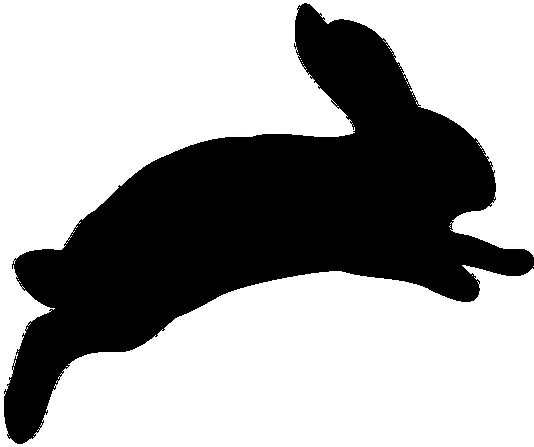
\includegraphics[height = .1\textheight]{rabbit_b}
%       };

%       \node<6->[
%       below = of p_t_false,
%       ] (t_p_t_false) {
%         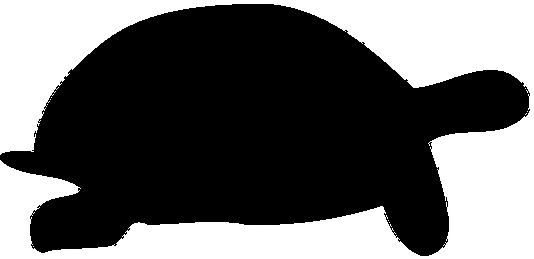
\includegraphics[height = .1\textheight]{turtle_b}
%       };

%       \node<9->[
%       below = of p_f_false,
%       ] (r_p_f_false) {
%         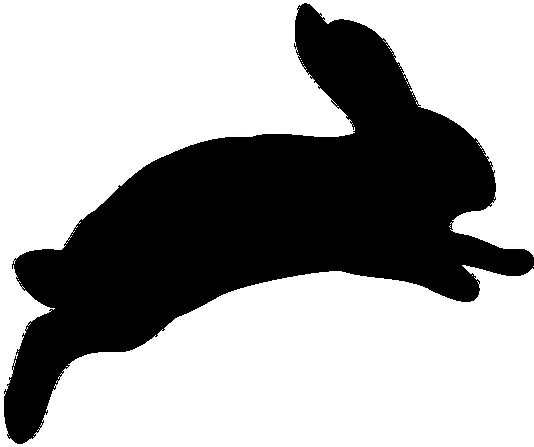
\includegraphics[height = .1\textheight]{rabbit_b}
%       };

%       \node<11->[
%       below = of p_f_true,
%       ] (q_p_f_true) {
%         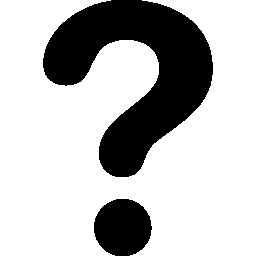
\includegraphics[height = .1\textheight]{question_b}
%       };

%       \draw<2-> (if_bound) -> (true);
%       \draw<3-> (true) -> (p_t_true);
%       \draw<4-> (p_t_true) -> (r_p_t_true);
%       \draw<5-> (true) -> (p_t_false);
%       \draw<6-> (p_t_false) -> (t_p_t_false);
%       \draw<7-> (if_bound) -> (false);
%       \draw<8-> (false) -> (p_f_false);
%       \draw<9-> (p_f_false) -> (r_p_f_false);
%       \draw<10-> (false) -> (p_f_true);
%       \draw<11-> (p_f_true) -> (q_p_f_true);

%     \end{tikzpicture}
%     % \caption{}\label{fig:exe_in_order}
%   \end{figure}

%   \note<1>{

%     Рассмотрим, в каких случаях происходит спекулятивное выполнение.

%   }

%   \note<2>{

%     Если чтение участка памяти происходит согласно заявленным границам.

%   }

%   \note<3>{

%     Чтение согласно границам, предсказатель также думал, что чтение будет
%     происходить согласно границам:

%     \begin{itemize}
%     \item спекулятивно выполнится код чтения в соответствии с границами памяти
%     \end{itemize}

%   }

%   \note<4>{

%     В итоге выполнение кода произойдёт быстро, так как уже заранее был выполнен,
%     результаты получены.

%   }

%   \note<5>{

%     Чтение согласно границам, предсказатель же думал, что чтение памяти выйдет
%     за границы.

%     \begin{itemize}
%     \item спекулятивно будет выполняться последующий за чтением памяти код
%     \item спекулятивное выполнение отбросится, выполнение кода будет происходить
%       заново
%     \end{itemize}

%   }

%   \note<6>{

%     В итоге из-за расхождения реальности с предсказанием, скорость выполнения
%     кода будет ниже.

%   }

%   \note<7>{

%     Если чтение участка памяти происходит за заявленными границами памяти.

%   }

%   \note<8>{

%     Чтение участка памяти за границами, предсказатель также думал, что чтение
%     будет происходить за границами.

%     \begin{itemize}
%     \item спекулятивно будет выполняться последующий за чтением памяти код
%     \end{itemize}

%   }

%   \note<9>{

%     Код исполнится быстро, так как предсказатель угадал и спекулятивно выполнял
%     последующий код.

%   }

%   \note<10>{

%     В случае же, если предсказатель ошибся и решил, что вычисления будут
%     происходить в границах памяти:

%     \begin{itemize}
%     \item спекулятивно выполнится код, который на практике выходит за границы
%       памяти
%     \end{itemize}

%   }

%   \note<11>{

%     \textbf{Спекулятивно выполнится код}, который на практике \textbf{выходит за
%       границы памяти}.

%   }

% \end{frame}

% \subsubsection{Тренировка предсказателя переходов}
% \begin{frame}[fragile]{\insertsubsubsection}

%   \begin{figure}[h]

%     \newcommand*\colorcone{Black}
%     \newcommand*\colorctwo{Black}
%     \newcommand*\colorcthree{Black}
%     \newcommand*\colorcfour{Black}
%     \newcommand*\colorcfive{Black}
%     \newcommand*\colorcsix{Black}
%     \newcommand*\colorcseven{Black}
%     \newcommand*\digitnum{0}

%     \only<2-3> {
%       \renewcommand*\colorcone{BrickRed}
%     }
%     \only<4-5> {
%       \renewcommand*\colorctwo{BrickRed}
%       \renewcommand*\digitnum{1}
%     }
%     \only<6-7> {
%       \renewcommand*\colorcthree{BrickRed}
%       \renewcommand*\digitnum{2}
%     }
%     \only<8-9> {
%       \renewcommand*\colorcfour{BrickRed}
%       \renewcommand*\digitnum{3}
%     }
%     \only<10-11> {
%       \renewcommand*\colorcfive{red}
%       \renewcommand*\digitnum{4}
%     }
%     \only<12-13> {
%       \renewcommand*\colorcsix{red}
%       \renewcommand*\digitnum{5}
%     }
%     \only<14-15> {
%       \renewcommand*\colorcseven{red}
%       \renewcommand*\digitnum{6}
%     }

%     \begin{tikzpicture}[
%       draw,
%       align = center,
%       ->,
%       > = Stealth,
%       thick,
%       double distance = 1pt,
%       node distance = .6,
%       block/.style = {
%         rectangle,
%         draw,
%         fill = ForestGreen,
%         text = White,
%         minimum width = 2cm,
%       },
%       ]

%       \node[
%       ] (code) {
%         \color{Black}index = \color{Mahogany}\digitnum\color{Black};\\
%         \color{Black}char* data = "\color{\colorcone}t\color{\colorctwo}e\color{\colorcthree}x\color{\colorcfour}t\color{\colorcfive}K\color{\colorcsix}E\color{\colorcseven}Y\color{Black}";\\
%         \color{Black}if (index < \color{Mahogany}4\color{Black})\\
%       };

%       \node[
%       below left = 3 of code,
%       text = Black,
%       font = \ttfamily,
%       minimum width = 3cm,
%       ] (cache) {
%         arr1[untrusted]
%       };

%       \node[
%       below = of code,
%       text = White,
%       fill = ForestGreen,
%       draw,
%       label = below:Предсказание,
%       ] (zero) {
%         $\omega = $\\
%         \only<1-2>{.50 | .50}%
%         \only<3-4>{.60 | .40}%
%         \only<5-6>{.69 | .31}%
%         \only<7-8>{.76 | .24}%
%         \only<9-10>{.81 | .19}%
%         \only<11-12>{.77 | .23}%
%         \only<13-14>{.70 | .30}%
%         \only<15>{.64 | .36}%
%       };

%       \node[
%       below right = 3 of code,
%       text = Black,
%       font = \ttfamily,
%       minimum width = 3cm,
%       ] (zero) {
%         0
%       };

%       \draw<1-2,11,13,15> (code) -> node[above, sloped] {true} (cache);
%       \draw<1,3-10,12,14> (code) -> node[above, sloped] {false} (zero);

%       \draw<2>[NavyBlue] (code) -> node[above, sloped] {false} node[below, sloped] {Спекулятивно} (zero);
%       \draw<3>[ForestGreen] (code) -> node[above, sloped] {true} node[below, sloped] {Реально} (cache);

%       \draw<4>[NavyBlue] (code) -> node[above, sloped] {true} node[below, sloped] {Спекулятивно} (cache);
%       \draw<5>[ForestGreen] (code) -> node[above, sloped] {true} node[below, sloped] {Реально} (cache);

%       \draw<6>[NavyBlue] (code) -> node[above, sloped] {true} node[below, sloped] {Спекулятивно} (cache);
%       \draw<7>[ForestGreen] (code) -> node[above, sloped] {true} node[below, sloped] {Реально} (cache);

%       \draw<8>[NavyBlue] (code) -> node[above, sloped] {true} node[below, sloped] {Спекулятивно} (cache);
%       \draw<9>[ForestGreen] (code) -> node[above, sloped] {true} node[below, sloped] {Реально} (cache);

%       \draw<10>[BrickRed] (code) -> node[above, sloped] {true} node[below, sloped] {Спекулятивно} (cache);
%       \draw<11>[ForestGreen] (code) -> node[above, sloped] {false} node[below, sloped] {Реально} (zero);

%       \draw<12>[BrickRed] (code) -> node[above, sloped] {true} node[below, sloped] {Спекулятивно} (cache);
%       \draw<13>[ForestGreen] (code) -> node[above, sloped] {false} node[below, sloped] {Реально} (zero);

%       \draw<14>[BrickRed] (code) -> node[above, sloped] {true} node[below, sloped] {Спекулятивно} (cache);
%       \draw<15>[ForestGreen] (code) -> node[above, sloped] {false} node[below, sloped] {Реально} (zero);

%     \end{tikzpicture}
%     % \caption{Неосознанная тренировка предсказателя переходов}
%   \end{figure}

%   \note<1>{



%   }

% \end{frame}

% \subsubsection{Обход проверки границ}
% \begin{frame}[fragile]{\insertsubsubsection}

%   \begin{minted}{c}
%     struct array {
%       unsigned long length;
%       unsigned char data[];
%     };
%     struct array *arr1 = ...; /* небольшой массив */
%     struct array *arr2 = ...; /* массив размером 0x400 */
%     unsigned long untrusted_offset_from_user = ...;
%     if (untrusted_offset_from_user < arr1->length) {
%       unsigned char value = arr1->data[untrusted_offset_from_user];
%       unsigned long index2 = ((value & 1) * 0x100) + 0x200;
%       if (index2 < arr2->length) {
%         unsigned char value2 = arr2->data[index2];
%       }
%     }
%   \end{minted}

%   \note{

%     Существует множество вариантов эксплуатации данной уязвимости, рассмотрим
%     одну из них.

%     Разберём всё по порядку.

%   }
% \end{frame}

% \begin{frame}[fragile]{\insertsubsubsection}

%   \begin{minted}{c}
%     struct array {
%       unsigned long length;
%       unsigned char data[];
%     };
%     struct array *arr1 = ...; /* небольшой массив */
%     struct array *arr2 = ...; /* массив размером 0x400 */
%   \end{minted}

%   \note{

%     Объявляется два массива.

%     Первый --- целевой массив, в котором будет происходить обход границ.

%     Второй --- массив для применения атаки на кэш.

%   }
% \end{frame}

% \begin{frame}[fragile]{\insertsubsubsection}

%   \begin{minted}{c}
%     /* переменная, управляемая атакующим */
%     unsigned long untrusted_offset_from_user = ...;

%     /* проверка границ */
%     if (untrusted_offset_from_user < arr1->length) {

%       /* спекулятивное выполнение, получение значения недоступной памяти */
%       unsigned char value = arr1->data[untrusted_offset_from_user];

%       /* получение значения бита интересующей области памяти */
%       unsigned long index2 = ((value & 1) * 0x100) + 0x200;

%       /* атака на кэш */
%       unsigned char value2 = arr2->data[index2];
%     }
%   \end{minted}

%   \note{

%     Проверка границ происходит как в примере представленном ранее.

%     Атака на кэш происходит как в примере, рассказанном ранее.

%     Код следующий за проверкой границ называется «гаджетом», как и в случае с
%     ROP.

%     Многое зависит от устройства кэшей различных уровней, TLB, BTB (branch
%     target buffers).

%   }
% \end{frame}

% \subsubsection{ASM}
% \begin{frame}[fragile]{\insertsubsubsection}

%   \begin{minted}{nasm}
%     LDR X1, [X2]      ; X2 - указатель на arr1->length
%     CMP X0, X1        ; X0 содержит untrusted_offset_from_user
%     BGE out_of_range
%     LDRB W4, [X5,X0]  ; X5 содержит arr1->data
%     AND X4, X4, #1
%     LSL X4, X4, #8
%     ADD X4, X4, #0x200
%     LDRB X7, [X8, X4] ; X8 содержит arr2->data
%     out_of_range
%   \end{minted}

%   \note{

%     Упрощённый asm код

%     Спекулятивно можно выполнить так же \textbf{ROP гаджеты}, заставить
%     выполнять операции, тем самым считывать данные из \textbf{закрытых
%       ресурсов}, например, крипто-чип.

%   }

% \end{frame}


\subsubsection{Предотвращение}
\begin{frame}{\insertsubsubsection}

  \begin{itemize}
  \item отключение спекулятивного выполнения
  \item ограничение доступа к высокоточным таймерам
  \item привилегированная очистка кэша
  \item полное изолирование важных данных
  \item вставка инструкций для остановки спекулятивного выполнения
  \end{itemize}

  \note{

    \begin{itemize}
    \item Как отключить? Большое проседание в производительности!
    \item сделали свои таймеры
    \item другие методы очистки
    \item spectre работает и на безопасных анклавах
    \item большое проседание по производительности + всё перекомпилировать
    \end{itemize}

  }

\end{frame}

% \subsection{Variant 2}
% \begin{frame}{\insertsubsection}

  CVE-2017-5715: тренировка предсказателя переходов

  \begin{figure}[h]
    
\includegraphics[height = .7\textheight]{spectre_logo}
    % \caption{Spectre}
  \end{figure}

  \note{


  }
\end{frame}

% \subsubsection{Предсказатель переходов и его тренировка}
% \begin{frame}{\insertsubsubsection}

%   \begin{figure}[h]
%     \begin{tikzpicture}[
%       align = center,
%       ->,
%       > = Stealth,
%       thick,
%       ampersand replacement = \&,
%       block/.style = {
%         rectangle,
%         draw,
%         fill = ForestGreen,
%         text = White,
%         text centered,
%       },
%       ]

%       \node[
%       text = Black,
%       font = \ttfamily,
%       ] (code) {
%         Animal* a = \color{ForestGreen}\only<1-4>{bird}\only<5->{fish};
%       };

%       \node[
%       below = .5 of code,
%       text = Black,
%       font = \ttfamily,
%       ] (move) {
%         a->move()
%       };

%       \node[
%       below left = 3 of move,
%       text = Black,
%       font = \ttfamily,
%       minimum width = 3cm,
%       ] (cache) {
%         arr1[untrusted]
%       };

%       \node[
%       circle,
%       below = of move,
%       text = White,
%       fill = ForestGreen,
%       draw,
%       label = below:Предсказание,
%       ] (zero) {
%         \only<1-3>{swim()}%
%         \only<4->{fly()}%
%       };

%       \node[
%       below right = 3 of move,
%       text = Black,
%       font = \ttfamily,
%       minimum width = 3cm,
%       ] (zero) {
%         0
%       };

%       \draw<1-2,4-5,7> (move) -> node[above, sloped] {fly()} (cache);
%       \draw<1,3,4-6> (move) -> node[above, sloped] {swim()} (zero);

%       \draw<2>[ForestGreen] (move) -> node[above, sloped] {swim()} node[below, sloped] {Спекулятивно} (zero);
%       \draw<3>[ForestGreen] (move) -> node[above, sloped] {fly()} node[below, sloped] {Реально} (cache);

%       \draw<6>[ForestGreen] (move) -> node[above, sloped] {fly()} node[below, sloped] {Спекулятивно} (cache);
%       \draw<7>[ForestGreen] (move) -> node[above, sloped] {swim()} node[below, sloped] {Реально} (zero);

%     \end{tikzpicture}
%     % \caption{}

%   \end{figure}

%   \note<1>{

%     Ранее уже рассказывалось про предсказатель переходов, а также про буфер.

%     Для атаки требуется досконально знать, \textbf{как работает предсказатель
%       переходов}.

%   }

%   \note<6>{

%     \textbf{Внимание}, спекулятивно выполняется натренированная нами ветка! В
%     итоге будет исполняться код, который совершит атаку на кэш.

%   }
% \end{frame}

% \begin{frame}{\insertsubsubsection}

%   \begin{figure}[h]
%     \begin{tikzpicture}[
%       align = center,
%       ->,
%       > = Stealth,
%       thick,
%       ampersand replacement = \&,
%       bp/.style = {
%         rectangle,
%         rectangle split,
%         rectangle split parts = 2,
%         rectangle split horizontal,
%         rectangle split part fill = {
%           ForestGreen, NavyBlue
%         },
%         draw,
%         text = White,
%       },
%       ]

%       \node[
%       bp,
%       ] (bp) {
%         \color{Black}0xEBE45A82
%         \nodepart{two}
%         T,T,N,N,T,T,N,N
%         \nodepart{three}
%       };

%       \node[
%       bp,
%       above left = of bp.center,
%       label = above:Процесс A,
%       ] (proc_a) {
%         0x0000 \color{Black}EBE45A82
%         \nodepart{two}
%         Переход A
%         \nodepart{three}
%       };

%       \node[
%       bp,
%       above right = of bp.center,
%       label = above:Процесс B (ядро/гипервизор),
%       ] (proc_b) {
%         0xFFFF \color{Black}EBE45A82
%         \nodepart{two}
%         Переход B
%         \nodepart{three}
%       };

%       \draw (proc_a.one south) |- (bp.one west);
%       \draw (proc_b.one west) -> (bp.one north);


%     \end{tikzpicture}
%     \caption{В BTB используются виртуальные адреса, а также возникают коллизии}

%   \end{figure}


%   \note{

%     Из-за того, что возникают коллизии в таблице BTB, мы можем
%     \textbf{натренировать} его таким образом, чтобы спекулятивно исполнялся
%     нужный нам переход.

%     Существует \textbf{не один способ} тренировки предсказателя переходов.

%     Также существует возможность создания ROP цепочки из \textbf{гаджетов
%       программы-жертвы} и натренировать на него, но для этого требуется знать
%     адрес. Чтобы \textbf{узнать адрес перехода} можно применить \textbf{атаку по
%       сторонним каналам} на предсказатель переходов.

%   }
% \end{frame}

% \subsubsection{И снова спекулятивное выполнение}
% \begin{frame}[fragile]{\insertsubsubsection}

%   \begin{minted}{c}
%   if (untrusted_offset_from_user < array1_size)
%     y = array2[((array1[untrusted_offset_from_user] & 1) * 0x100) + 0x200];
%   \end{minted}

%   \note{

%     Ничего нового, используется всё тот же код, чаще всего ROP цепочка, которая
%     приводит к атакам на кэш.

%   }
% \end{frame}

\subsubsection{Предотвращение}
\begin{frame}{\insertsubsubsection}

  Частично такое же, как и в случае с Variant 1

  \begin{itemize}
  \item отключение предсказателя переходов
  \item очистка буфера предсказателя переходов при переключении контекста
  \item вставка «барьеров» (Indirect Branch Restrict Speculation, Indirect
    Branch Predictor Barrier и др.)
  \item retpoline --- «оборачивание» косвенных переходов
  \item oo7 --- умное «оборачивание» косвенных переходов
  \end{itemize}

  \note{

    Всё медленно!

    retpoline --- замена всех косвенных переходов, дополнение инструкций
    возврата, паузы перед непрямыми вызовами функций

  }

\end{frame}

% \subsection{Variant 4}
% \begin{frame}{\insertsubsection}

  CVE-2018-3639: спекулятивное выполнение чтения памяти после сохранения её в
  регистр

  \begin{figure}[h]
    
\includegraphics[height = .7\textheight]{spectre_logo}
    \caption{Spectre}
  \end{figure}

  \note{


  }
\end{frame}

\subsubsection{Сначала чтение, потом запись}
\begin{frame}[fragile]{\insertsubsubsection}
  \begin{minted}{nasm}
    STR X1, [X2]   ; X2 - адрес памяти, который ещё не известен
    ...
    LDR X3, [X4]   ; X4 содержит тот же адрес, что и X2
    <произвольная обработка X3>
    LDR X5, [X6, X3]  ; спекулятивное выполнение со старым адресом
  \end{minted}

  \note{

    Во многих современных процессорах применяются интересные техники
    оптимизации, а именно: \textbf{загрузка данных} из памяти по определённому
    адресу производится \textbf{раньше, чем запись} в тот же участок памяти в
    случае, \textbf{если адрес} на этапе записи данных \textbf{ещё не известен}.

    В итоге у нас \textbf{спекулятивно выполняются} все операции \textbf{со
      старым адресом} в регистре (в том числе запись в кэш).

  }
\end{frame}

\subsubsection{Читаем данные EL1}
\begin{frame}[fragile]{\insertsubsubsection}
  \begin{minted}{nasm}
    STR X1, [X2]
    ...
    ERET           ; возврат на более нижний уровень исключений
    ...
    LDR X3, [X4]   ; X4 содержит такой же физический адрес, как и X2,
                   ; но виртуальный адрес отличается
    <произвольная обработка X3>
    LDR X5, [X6, X3]
  \end{minted}

  \note{

    Если \textbf{адрес один и тот же} (виртуальный и физический), то данная
    уязвимость эксплуатируема только \textbf{на одном уровне исключений}
    (exception level for ARM).

    В случае, если есть возможность \textbf{чтения на одном уровне исключений},
    а \textbf{загрузки на другом}, и при этом используется \textbf{один и тот же
      физический адрес}, то есть возможность эксплуатации уязвимости \textbf{на
      разных уровнях}.

  }
\end{frame}

\subsubsection{Спекулятивное чтение одного и того же регистра}
\begin{frame}[fragile]{\insertsubsubsection}
  \begin{minted}{nasm}
    STR X1, [SP]
    ...
    LDR X3, [SP]
    <произвольная обработка X3>
    LDR X5, [X6, X3]
    <произвольная обработка X5>
    LDR X7, [X8, X5]
  \end{minted}

  \note{

    Удивительно, но факт --- мы можем читать данные из памяти, обращаясь по
    одному и тому же регистру.

    Такое возможно благодаря \textbf{современным оптимизациям на некоторых
      архитектурах}. В случае, если у нас содержимое SP, например,
    \textbf{отсутствовало в кэше}, то \textbf{при записи} мы получим
    \textbf{cache miss} и задержку, позволяющую нам \textbf{спекулятивно
      прочитать всё те же данные}. Такое возможно по причине того, что процессор
    в RoB отслеживает, когда данные из регистра попали в кэш и соответственно
    ускоряет исполнение инструкций.

    \textbf{PoC нет!}

  }
\end{frame}

\subsubsection{Спекулятивный запуск непривилегированного кода}
\begin{frame}[fragile]{\insertsubsubsection}
  \begin{minted}{nasm}
    STR X1, [SP]
    ...
    LDR X3, [SP]
    ...
    BLR X3
  \end{minted}

  \note{

    Так же, как и в обычном Spectre, мы можем составить цепочку ROP гаджетов и
    спекулятивно их запустить, чтобы \textbf{записать нужные нам данные в кэш}.

  }
\end{frame}

\subsubsection{Сначала запись, потом чтение}
\begin{frame}[fragile]{\insertsubsubsection}
  \begin{minted}{nasm}
    ...
    LDR X3, [X4]
    <произвольная обработка X3>
    LDR X5, [X6, X3]
    ....
    STR X1, [X2] ; X2 содержит тот же адрес, что и X4
  \end{minted}

  \note{

    Утверждается, что существует возможность прочитать данные спекулятивно,
    записанные также спекулятивно, но позже. Это возможно в случае, если регистр
    для чтения будет высчитываться гораздо дольше регистра для записи.

    \textbf{PoC нет!}

  }
\end{frame}

\subsubsection{Предотвращение}
\begin{frame}{\insertsubsubsection}

  \LARGE

  \begin{itemize}
  \item вставка «барьеров»
  \item отключение реорганизации операций чтения и записи
  \item SafeSpec
  \end{itemize}

  \note{

    Медленно!

  }

\end{frame}


\subsection{Derived attacks and not only}
\begin{frame}{\insertsubsection}

  Spectre-NG
  \begin{itemize}
  \item MeltdownPrime \& SpectrePrime
  \item SgxPectre
  \item SMM Speculative Execution Attacks
  \item BranchScope
  \item LazyFP
  \item TLBleed
  \item ...
  \end{itemize}

  TotalMeltdown?

  \note{

    \textbf{OpenBSD} --- LazyFP, отключение Hyper-Threading (TLBleed).

    \begin{itemize}
    \item \textbf{другой способ атаки на кэш} + задействование двух ядер CPU ---
      утечка данных работы \textbf{протокола согласования содержимого кэша для
        разных ядер CPU} (Invalidation-Based Coherence Protocol
    \item позволяет обойти средства изоляции кода и данных, предоставляемые
      технологией \textbf{Intel SGX} (Software Guard Extensions)

      SMM --- \textbf{режим системного управления} --- запускается специальная
      программа в привилегированном режиме.

    \item \textbf{variant 2} + вместо BTB --- \textbf{направления ветвления для
        спекулятивного перехода (directional branch predictor)} и манипулирует
      содержимым \textbf{таблицы с историей шаблонов переходов (PHT, Pattern
        History Table)}.
    \item \textbf{variant 3a} --- «ленивое» режим \textbf{переключения контекста
        FPU}, при котором реальное восстановление состояния регистров
      производится \textbf{не сразу} после переключения контекста, а только при
      выполнении первой инструкции
    \item ML атака на TLB, с помощью Hyper-Threading технологии (Intel, AMD).
    \end{itemize}

  }

\end{frame}


\subsection{Abstract example of exploitation}
\begin{frame}{\insertsubsection}

  \newcommand{\insm}{%
    \smash{\raisebox{1.8\dimexpr1\baselineskip+4\itemsep+2\parskip}{$\left.\rule{0pt}{.5\dimexpr9\baselineskip+3\itemsep+3\parskip}\right\}$\
        \parbox{5.5cm}{Microarchitecture --- ?}}} }


  \only<1-2, 4-5, 7-8, 10-11>{

    The four components of speculation techniques

    \begin{enumerate}
    \item<1-|alert@1-2> Speculation primitive
    \item<4-|alert@4-5> Windowing gadget
    \item<7-|alert@7-8> Disclosure gadget
    \item<10-|alert@10-> Disclosure primitive
    \end{enumerate}
  }

  \note<1>{

    А так ли всё легко и просто? Представим, что мы хотим совершить атаку.

    Рассмотрим на примере Spectre v2 (variant 2).

    Процессор \textbf{должен поддерживать} возможность спекулятивного
    выполнения.

    Требуется \textbf{найти место} в коде, где может происходить спекулятивное
    выполнение по желанию атакующего.

  }

  \note<4>{

    Требуется найти гаджеты, которые позволят создать достаточно
    \textbf{длительное по времени выполнения окно} для спекулятивного
    выполнения.
    
  }

  \note<7>{

    Требуется найти гаджеты, которые позволят \textbf{считать необходимую
      закрытую информацию} в ходе спекулятивного выполнения.
    
  }

  \note<10>{

    Требуется возможность \textbf{считать полученную} через сторонний канал
    информацию или \textbf{удостовериться}, что она была считана.

  }

  \only<3, 6, 9, 12>{
    \begin{figure}[h]
      \begin{tikzpicture}[
        align = center,
        ->,
        > = Stealth,
        thick,
        block/.style = {
          draw,
          fill = ForestGreen,
          text = White,
        },
        ]

        \node[
        block,
        ] (type_bp) {
          Type of BP
        };

        \node[
        block,
        right = of type_bp,
        rotate = 3,
        ] (algo_bp) {
          Algorithm of BP
        };

        \node[
        block,
        right = of algo_bp,
        rotate = -2,
        ] (work_bp) {
          Environment of BP
        };

        \node<6->[
        block,
        above = 0 of $(type_bp.north)!0.5!(algo_bp.north)$,
        rotate = 2,
        ] (search_cache_gadgets) {
          Search/create gadgets
        };

        \node<6->[
        block,
        above = .13 of $(work_bp.north)!0.5!(algo_bp.north)$,
        % rotate = 1,
        ] (info_cache) {
          Contents of cache
        };

        \node<9->[
        block,
        above = .05 of $(search_cache_gadgets.north)!0.5!(info_cache.north)$,
        rotate = 4,
        ] (bypass_aslr) {
          Bypass ASLR
        };

        \node<9->[
        block,
        above = 0 of info_cache.north east,
        rotate = -8,
        ] (bypass_others) {
          Bypass others techniques
        };

        \node<12->[
        block,
        above = 1.7 of search_cache_gadgets,
        rotate = 65,
        ] (timers) {
          High-resolution timer
        };

        \node<12->[
        block,
        above = -0.5 of bypass_aslr,
        minimum width = 5cm,
        minimum height = 2cm,
        fill opacity = 0.5,
        text opacity = 1,
        text = Black,
        ] (noise) {
          Noise
        };

        \node<12->[
        block,
        above = 0 of noise,
        ] (flush_reload) {
          Flush + Reload
        };

        \node<12->[
        inner sep = 0,
        above = 1 of bypass_others.east,
        ] (vovka) {
          
\includegraphics[width = .15\textwidth]{vovka}
        };

      \end{tikzpicture}
      \only<1-5>{\caption{Foundation of tower\\\textit{speculative-based
            attack}}}

      \only<6-8>{\caption{Tower\\\textit{speculative-based attack}}}

      \only<9->{\caption{\textbf{Babel} tower\\\textit{speculative-based
            attack}}}
    \end{figure}
  }

  \note<3>{

    Выберем тренировку предсказателя переходов. Мы столкнёмся:

    \begin{itemize}
    \item требуется знать \textbf{вид предсказателя переходов}
    \item требуется знать \textbf{алгоритм работы предсказателя переходов}
    \item для \textbf{разных процессоров --- разные условия}, например, в i7 два
      буфера предсказателя переходов.
    \end{itemize}

    В whitepaper и в PoC даны \textbf{примеры для конкретных процессоров}.

  }

  \note<6>{

    Выберем гаджеты для загрузки некэшированных данных. Мы столкнёмся:

    \begin{itemize}
    \item в случае JIT --- создание гаджетов, в других случаях гаджеты следует
      искать,
    \item что хранится в кэше на данный момент.
    \end{itemize}

    В whitepaper и в PoC даны \textbf{примеры для конкретных процессоров}.

  }

  \note<9>{

    В whitepaper и в PoC \textbf{все защиты отключены}.

  }

  \note<12>{

    Что? Ещё одна атака?

  }

  \only<2>{

    \begin{itemize}
    \item Bypass out of bounds checks
    \item Training of branch predictor
    \item Speculatively read an earlier value of the data
    \item Pending exceptions
    \item Exploit branch history table
    \item Exploit the Return Stack Buffer
    \item Speculatively write to register (buffer overflow) \insm
    \end{itemize}
    
  }

  \note<2> {

    На данный момент существует несколько техник, позволяющих производить
    спекулятивное выполнение по желанию атакующего.

    Для того, чтобы использовать те или иные техники \textbf{требуется
      досконально знать микроархитектуру процессора}.
    
  }

  \only<5>{

    \begin{itemize}
    \item Non-cached loads
    \item Dependency chain of loads
    \item Dependency chain of integer ALU operations
    \end{itemize}
    
  }

  \note<5>{

    Не \textbf{везде есть такие цепочки} в окружении. В некоторых случаях
    \textbf{требуется знать, какие данные сейчас в кэше}.
    
  }

  \only<8>{

    \begin{itemize}
    \item ASLR
    \item CFI
    \item SMAP
    \item DEP/NX
    \item retpoline
    \item and others.
    \end{itemize}
    
  }

  \note<8>{

    Для применения необходимых гаджетов требуется обойти некоторые системы
    защиты.
    
  }

  \only<11>{

    \begin{itemize}
    \item Architecture of cache
    \item Replacement policies
    \item Exclusive and inclusive
    \item Type of cache attack
    \item Noise
    \item High-resolution timer
    \item and etc.
    \end{itemize}

  }

  \note<11>{

    \begin{itemize}
    \item Требуется знать, какой тип кэша используется.
    \item Требуется знать, какие данные сейчас хранятся в кэше, как выталкивать.
    \item На какой кэш будет направлена атака.
    \item Возможность проведения той или иной атаки.
    \item Возможность многократного повторения атаки.
    \item Для измерения времени требуются высокоточные счётчики.
    \end{itemize}

  }

\end{frame}


% ------------------------------------------------------------------------------

\section{Summary}
\begin{frame}{\insertsection}

  \begin{itemize}[<+->]
  \item атаки на микроархитектуру становятся \textbf{популярными}
  \item атаки на микроархитектуру могут быть \textbf{автоматизированы}
  \item множество атак ещё \textbf{не опубликовано/найдено}
  \item создание контрмер --- \textbf{не тривиальный процесс}
  \end{itemize}

  \note<1>{

    Всё больше исследований проводится в этой области, всё больше обычных
    обывателей интересуются данной проблемой. Уязвимости в ПО \textbf{всё
      сложнее эксплуатировать, переходим к железу}.

    Уязвимости находят, \textbf{прочитав и разобравшись в спецификации
      архитектуры}, процессора. Обратную разработку производят с помощью базовых
    атак по сторонним каналам.
    
  }

  \note<2>{

    Представлено множество работ и инструментов, позволяющих провести атаку
    практически на любую популярную архитектуру. \textbf{Создаются
      эксплоит-паки}, содержащие атаки на микроархитектуру.
    
  }

  \note<3>{

    Описание атак, использующих спекулятивное выполнение, ещё \textbf{не до
      конца опубликованы}.

    Множество возможных \textbf{изъянов микроархитектуры не найдены}.
    
  }

  \note<4>{

    Для исправления сложившейся ситуации требуются \textbf{фундаментальные
      изменения} в ходе работы процессора.

    Исправления, \textbf{разработанные на уровне ОС}, требуют \textbf{детального
      изучения уязвимости} и алгоритма противодействия, к тому же \textbf{не
      всегда возможно предотвратить} эксплуатацию на уровне ОС, а если и
    удаётся, то в большинстве случаев приносят \textbf{в жертву процессы
      оптимизации}.
    
  }

\end{frame}


\begin{frame}[allowframebreaks]{References}

  \nocite{*}

  \bibliographystyle{ieeetr}
  \bibliography{main}

\end{frame}

\end{document}
